\documentclass[
12pt, % Main document font size
a4paper
%, % Paper type, use 'letterpaper' for US Letter paper
%oneside, % One page layout (no page indentation)
%twoside, % Two page layout (page indentation for binding and different headers)
%headinclude,footinclude, % Extra spacing for the header and footer
%BCOR5mm, % Binding correction
]{report}

\usepackage[font=small,labelfont=bf,justification=raggedright,format=hang,singlelinecheck=off,textfont=it]{caption}
%\usepackage{subcaption}
\usepackage{indentfirst}
\usepackage{longtable}
\usepackage{tabu}
\usepackage{titlepic}
\usepackage{geometry}
\geometry{margin=1in,top=1.5in,bottom=1.5in}
\usepackage{mathtools}
\usepackage{polski}
\usepackage[utf8]{inputenc}
\usepackage{booktabs}
\usepackage[T1]{fontenc}
\usepackage{lmodern}
\usepackage{fancyhdr}
\pagestyle{fancy}
\pagestyle{headings}
\usepackage{float}
\usepackage{graphicx}
\usepackage{listings}
\usepackage{enumitem}
\usepackage{titlesec}
\usepackage{pdfpages}
\usepackage{wallpaper}
%\usepackage{cleveref}
\usepackage{afterpage}

\usepackage{hyperref}
\hypersetup{
    colorlinks,
    citecolor=black,
    filecolor=black,
    linkcolor=black,
    urlcolor=black
}

\usepackage{cleveref}

\newcommand\blankpage{%
    \null
	\ClearWallPaper
    \thispagestyle{empty}%
    \addtocounter{page}{-1}%
    \newpage
	\ULCornerWallPaper{1}{head}}

%\captionsetup{}

%\usepackage{showframe}


\newcounter{magicrownumbers}
\newcommand\rownumber{\stepcounter{magicrownumbers}\arabic{magicrownumbers}}

%variables
\newcommand{\shopname}{SHOP NAME}
\newcommand{\companyname}{COMPANY NAME}
\newcommand{\regon}{REGON}
\newcommand{\nip}{NIP}
\newcommand{\httpaddr}{SITE ADDRESS}
\newcommand{\address}{ADDRESS}
\newcommand{\mail}{MAIL ADDRESS}
\newcommand{\phone}{PHONE NUMBER}
\newcommand{\currency}{CURRENCY}

\setlistdepth{9}
\graphicspath{ {images/} }

\title{Biznes plan sklep-meblowy.org}
\author{Kamila Klonowska <kamila.klon@sklep-meblowy.org>}
\titlepic{
\includegraphics[width=128px]{logo.png}}

%definitions
\newif\ifpersonal
\personaltrue % comment out to hide answers

%styling
\titlespacing*{\subparagraph}{1em}{0pt}{0pt}
\titleformat{\subparagraph}[runin]
{\normalfont\normalsize}{\thesubparagraph}{1em}{}

\ULCornerWallPaper{1}{head}
%\LLCornerWallPaper{1}{foot}

\begin{document}			


	%strona tytulowa
	\begin{titlepage}
	\clearpage\maketitle
	\thispagestyle{empty}
\end{titlepage}


	\afterpage{\blankpage}
	
	%spis tresci
	% Set the depth of the table of contents to show sections and subsections only
%\setcounter{tocdepth}{2} 
\newpage 
\tableofcontents % Print the table of contents
\newpage


	%pojecia
	\chapter*{Wstęp}
		\addcontentsline{toc}{chapter}{Wstęp}
		\section*{Definicje}
\addcontentsline{toc}{section}{Pojęcia}
	Pojęcia z jakimi należy się zaznajomić:
	\begin{description}
	
		\item[\textbf{Pojęcie}] - opis

	\end{description}

						
	\chapter{Opis przedsięwzięcia}
			\section{Wstęp} 
		\par Niniejszy dokument przedstawia biznes plan sklepu internetowego. Zawiera on opis wszystkich narzędzi niezbędnych do zarządzania i funkcjonowania takiego sklepu. Znajdziemy tu: plan finansowy i rozwojowy; analizę rynków sprzedaży w Polsce i Kanadzie; analizę branży meblarskiej; szczegółowe informacje na temat sprzętu niezbędnego do prowadzenia bezpiecznego i wydajnego sklepu internetowego. W dokumencie znalazły się także regulaminy w języku angielskim i polskim; karty gwarancyjne; informacje dotyczące polityki cookies. 
	
		\par Dokument ten, powstał z chęci przybliżenia zagadnień związanych z funkcjonowaniem coraz popularniejszych sklepów internetowych. Skupia się on na branży meblarskiej, która rokrocznie zwiększa swoje udziały w rynku. Sklep jaki pragnę stworzyć będzie zrzeszać niewielkich rzemieślników , fachowców mogących sprostać oczekiwaniom coraz bardziej wymagających klientów.
	
	\section{Specyfikacja przedsiębiorstwa}
		\begin{description}
			\item Data rozpoczęcia działalności - 01.06.2017
			\item Rodzaj działalności - handel
			\item Zakres działalności - PKD 47.91.Z  Sprzedaż detaliczna prowadzona przez domy sprzedaży wysyłkowej lub Internet	
			\item Sprzedaż produktów - rejestrowana za pomocą kasy fiskalnej
			\item Rozliczenie podatku dochodowego - książka przychodów i rozchodów
			\item Rozliczenie podatku VAT - podatnik Vat
		\end{description}
	
	\section{Wykształcenie; doświadczenie zawodowe; szkolenia}
	\subsection{Wykształcenie}
		\begin{itemize}
			\item 2008-2014 Wyższa Szkoła Zarządzania Edukacja; kierunek „Dziennikarstwo i komunikacja społeczna”
         \item 2000-2004 III Liceum Ogólnokształcące w Świdnicy 
		\end{itemize}
		
	\subsection{Doświadczenie zawodowe}
		\begin{itemize}
			\item 1.03.2012 - 31.10.2016 Kazar Footwear Sp. z o.o. - handlowiec/menadżer
			\item 20.02.2008 - 31.05.2011 Wittchen S.A. - sprzedawca, kierownik
			\item 27.03.2007 - 18.06.2007 Reserved LPP S.A. - sprzedawca  
		\end{itemize}	
		
	\subsection{Przebyte szkolenia}
		\begin{itemize}
			\item szkolenia w ramach projektu unijnego: księgowość, kadry i płace, ABC przedsiębiorczości, biznes plan,  ubezpieczenia społeczne, prawo podatkowe
			\item szkolenie dla kadry kierowniczej z zakresu BHP
			\item szkolenia wewnętrzne w firmach z zakresu zarządzania, technik sprzedaży, marketingu
		\end{itemize}
		
	\section{Podstawowe cele działalności}
		\par Głównym celem planowanej działalności gospodarczej, będzie internetowa działalność handlowa w branży meblowej. Określana także mianem działalności e-commerce w branży meblowej. Będzie ona skupiać się na sprzedaży eksportowej mebli pochodzących od małych i średnich producentów z Polski na teren Kanady, jak i na sprzedaży na rynku polskim. Główne nakłady pracy skupione będą na eksporcie ze względu na dochodowość tego rynku.
			
		\par Przedmiotem handlu na terytorium Polski i Kanady będą meble domowe. Handel odbywać będzie się poprzez portale aukcyjne i sklep internetowy. Zarówno obsługa ogłoszeń jak i sklepu internetowego będzie przebiegać w języku polskim i angielskim. Procesy jakie należy wykonać to: proces obsługi klienta, proces reklamacji, proces promocji. W procesie obsługi klienta składający zamówienie będą mieli możliwość dostosowania produktu do swoich potrzeb. Produkt prezentowany na stronie internetowej lub ogłoszeniu, to jedynie wzór produktu do wykonania. Dla tak skonfigurowanego produktu utworzone zostanie zlecenie produkcji. Produkt zostanie wykonany przez producenta według zamówienia i dostarczony do klienta. W procesie reklamacji należy przyjąć lub odrzucić zgłoszenie klienta oraz podjąć działania zmierzające do wyeliminowania wad produktu lub odrzucenia roszczeń. 
			
		\par Prowadzenie tego typu działalności wymaga wykonywania określonych zadań, do których należy obsługa klientów i producentów, promocja sklepu, sporządzanie statystyk.  Jak również pozyskanie środków sprzętowych, celem wprowadzenia odpowiedniej organizacji tych zadań. Koncept działalności przestawia następująca mapa:
			
		\begin{figure}[H]
			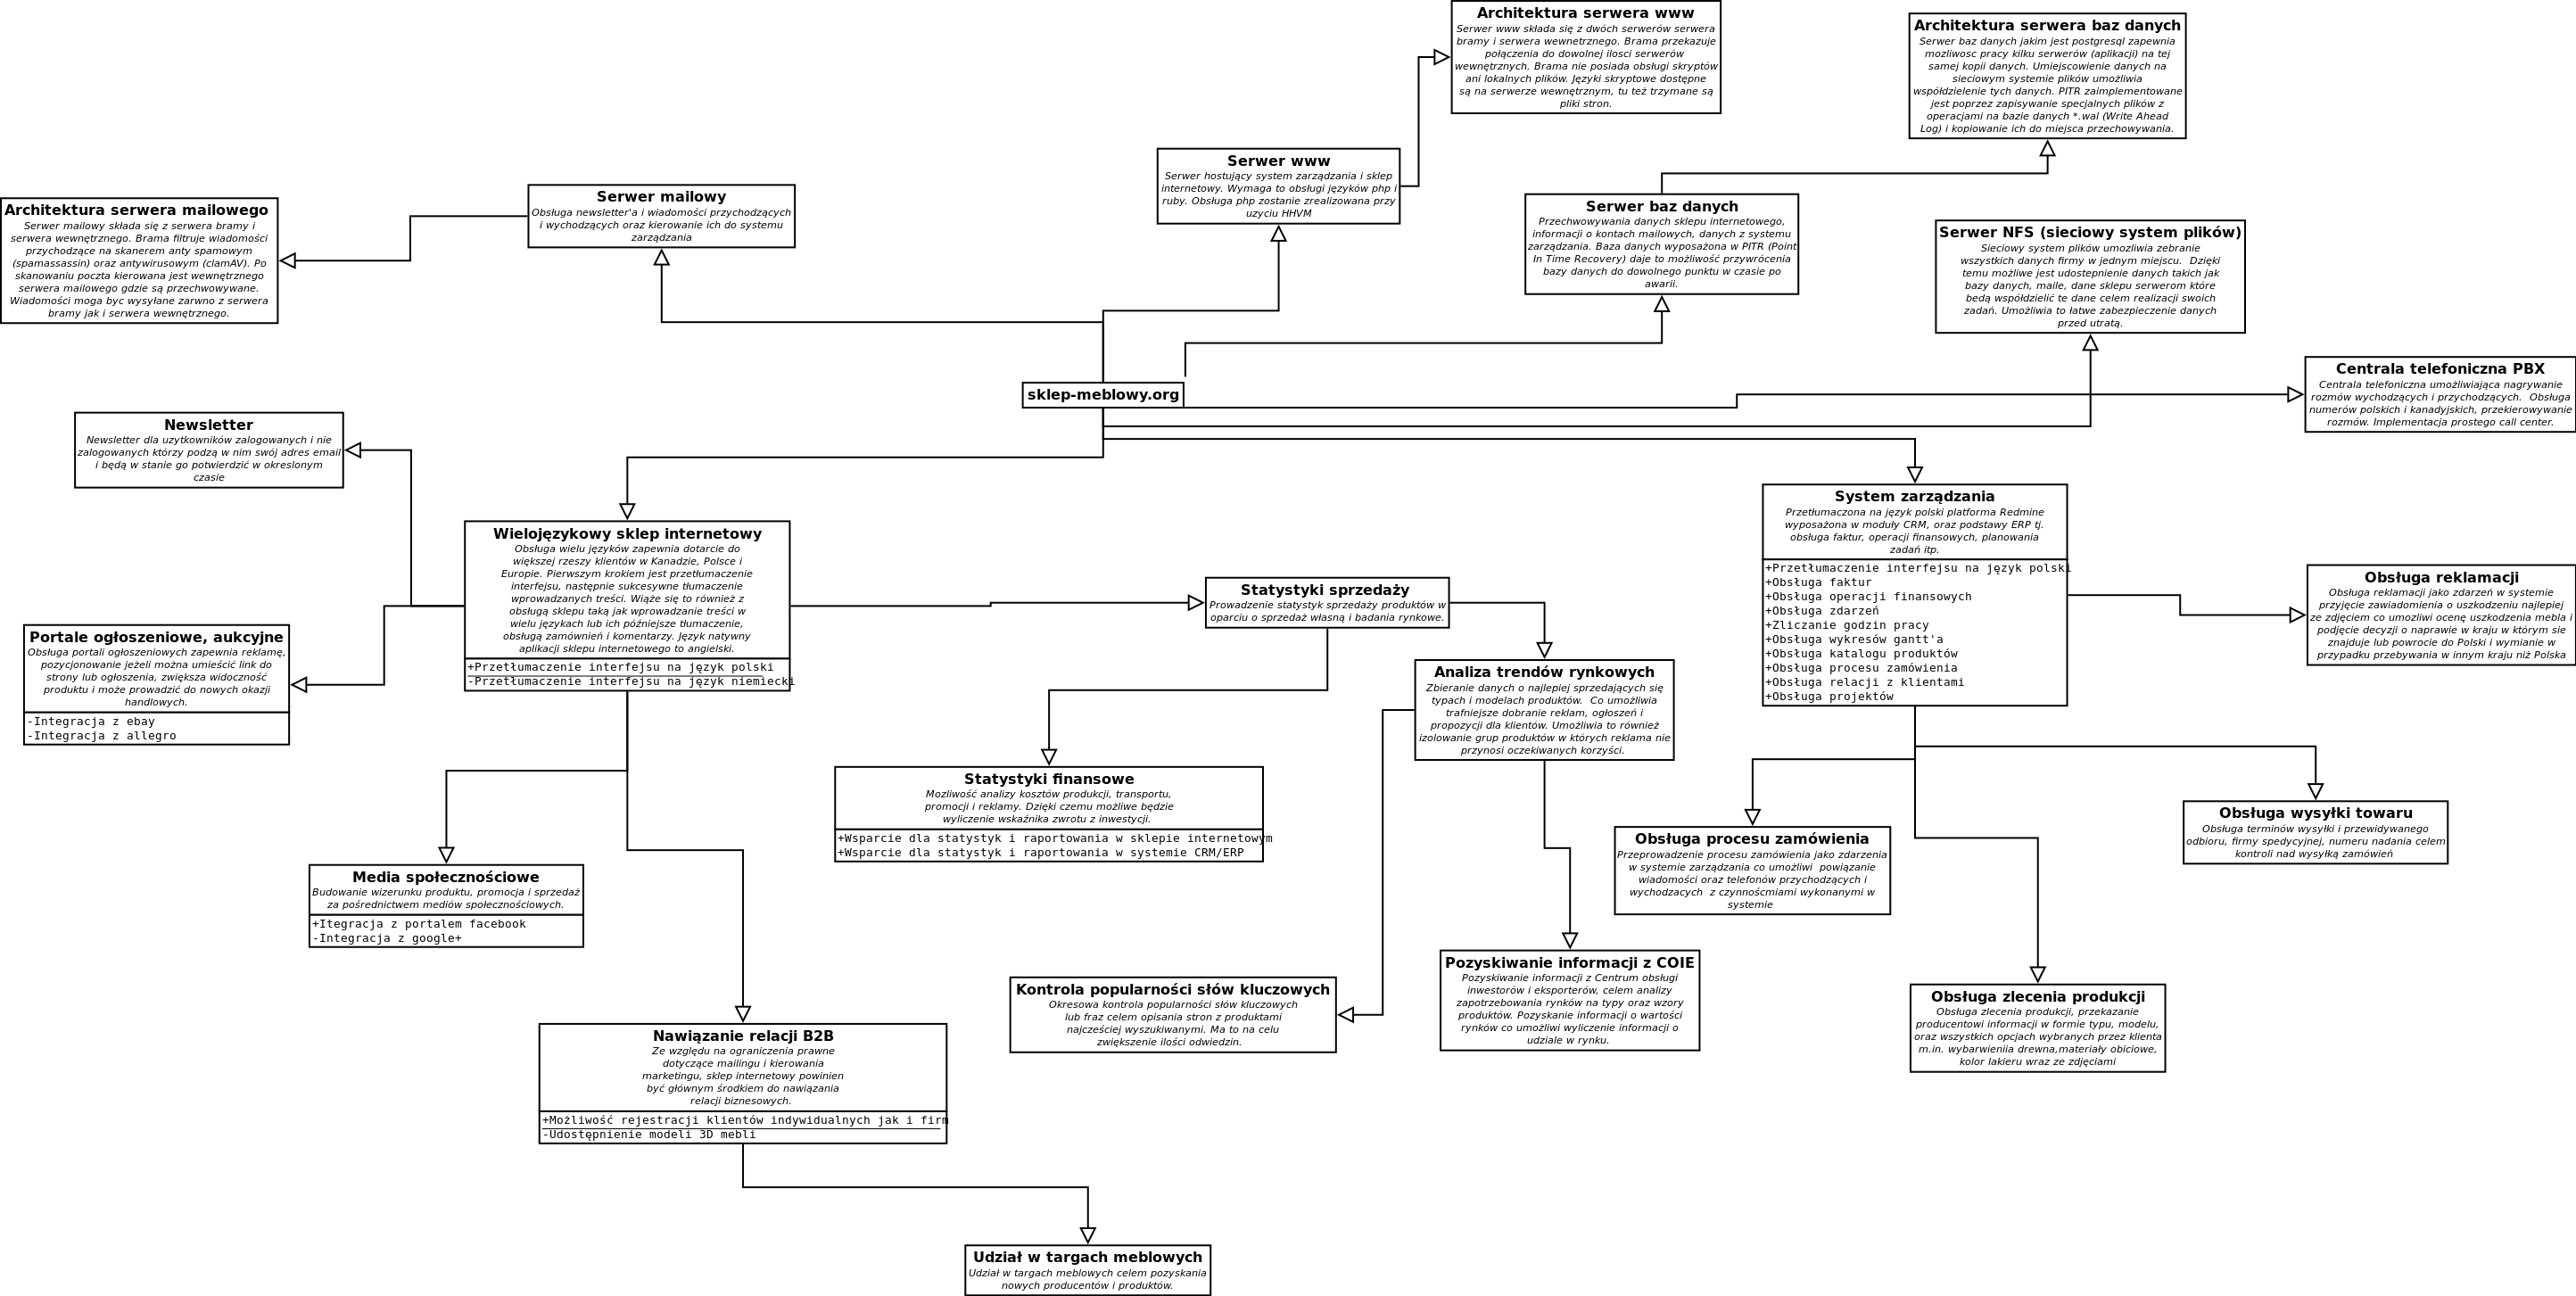
\includegraphics[scale=0.25,angle=90]{mindmap}
			\caption{Mapa projektu przedstawiająca konspekt środków, zadań i organizacji}
		\end{figure}
		
	\section{Oferowane usługi}
		\subsubsection{Usługa sprzedaży} 
			\par Przedmiotem podejmowanej działalności będzie internetowy sklep meblowy, oferujący sprzedaż asortymentu polskich wytwórców meblowych na rynku polskim jak i rynkach zagranicznych (ze szczególnym uwzględnieniem Kanady). Głównym produktem będą meble drewniane i tapicerowane. Po analizie rynku udało się ustalić, że przewagą mebli produkowanych w Polsce jest ich wysoka jakość oraz niska cena. Planuje być przede wszystkim pośrednikiem między wymagającymi, szukającymi wysokiej jakości klientami, a producentami tych dóbr, którzy w dużej mierze sami nie potrafią przebić się na szeroki rynek zbytu lub mają zbyt mały budżet na organizację kampanii reklamowej.
				
			\par Na stronie internetowej znajdować się będą istniejące wzory mebli od producentów wraz z możliwością ich dostosowania pod indywidualne wymagania klienta. Kluczowe jest więc zebranie jak największej liczby materiałów obiciowych, rodzajów drewna i jego wybarwień, okuć itp. tak, aby klient miał możliwość wpływu na powstanie produktu. Taki zabieg daje jeszcze jedną przewagę zarówno w świetle polskiego jak i kanadyjskiego prawa, ponieważ nie ma możliwości zwrotu towaru mocno spersonalizowanego.
				
		\subsubsection{Usługa reklamacji} 
			\par Drugą oferowaną usługą jest proces reklamacji. Usługa ta przeznaczona będzie dla klientów, u których wystąpią wady produktu w trakcie użytkowania lub produkt będzie niezgodny z zamówieniem. Na proces reklamacji składać się będzie przesłanie zdjęć wadliwego towaru przez klienta. Na podstawie tych zdjęć musi nastąpić decyzja o uznaniu lub odrzuceniu reklamacji. W przypadku uznania reklamacji w Polsce, należy zwrócić towar do producenta celem wykonania  niezbędnych napraw. W przypadku sprzedaży zagranicznej naprawa musi zostać wykonana na miejscu, co może wiązać się z koniecznością dosłania części zamiennych. Jeżeli naprawa nie jest możliwa na miejscu, produkt zostanie zwrócony do producenta lub wymieniony (w wypadku gdy koszty logistyki od klienta do producenta i z powrotem przekroczą wartość produktu).

	\section{Charakterystyka produktów}
		\par Moim celem jest zaprezentowanie produktów pochodzących od polskich producentów mebli, których wyróżnia jakość  użytych materiałów, dbałość o szczegóły i bardzo dobre wykonanie. Zależy mi aby wyjść naprzeciw oczekiwaniom współczesnego klienta, któremu co raz częściej zależy na produkcie mocno zindywidualizowanym. Dlatego klient sam będzie mógł dobrać sobie atrybuty produktu. Sprzedawanymi produktami będą meble domowe, w skład których wchodzą: 
	
		\begin{itemize}
			\item{sofy}
                \begin{itemize}
                    \item skórzane
                    \item tapicerowane
                    \item rozkładane
                    \item narożniki
                \end{itemize}
				
				\item{fotele}
					\begin{itemize}
					\item obrotowe
					\item skórzane
					\item tapicerowane
					\item z podnóżkiem
					\end{itemize}
					
            \item{łóżka}
                \begin{itemize}
                    \item drewniane
                    \item tapicerowane
                    \item podwójne
                    \item pojedyncze
                \end{itemize}
					
            \item{krzesła}
                \begin{itemize}
                    \item drewniane
                    \item obrotowe
                    \item biurowe
                    \item skórzane
                    \item hokery
                \end{itemize}
					
				\item{stoły}
                \begin{itemize}
                    \item drewniane
                    \item wysoki połysk
                    \item szklane
                    \item okrągłe
                \end{itemize}
					
				\item{stoliki kawowe}
                \begin{itemize}
                    \item drewniane
                    \item wysoki połysk
                    \item okrągłe
                    \item prostokątne
                \end{itemize}
					
				\item{szafki nocne}
                \begin{itemize}
                    \item drewniane
                    \item wysoki połysk
                \end{itemize}
					
				\item{szafki RTV}
                \begin{itemize}
                    \item drewniane
                    \item wysoki połysk
                    \item wiszące
                    \item stojące
                \end{itemize}
					
            \item{regały}
                \begin{itemize}
                    \item drewniane
                    \item wysoki połysk
                    \item stojące
                    \item wiszące
                \end{itemize}
				
            \item{biurka}
                \begin{itemize}
                    \item drewniane
                    \item wysoki połysk
                \end{itemize}
				
            \item{komody}
                \begin{itemize}
                    \item drewniane
                    \item wysoki połysk
                    \item niskie
                    \item wysokie
                \end{itemize}
		\end{itemize}
	
		\par Meble mogą być wykonane lub posiadać wykończenie z różnych materiałów. Poniżej zaprezentowane zostaną materiały, z których mogą być wykonane meble:
		
		\begin{itemize}
			\item{Drewno i płyty drewniane}
				\begin{itemize}
					\item{Drewno sosnowe} - jest sprężyste, wytrzymałe, posiada kremowe, szerokie usłojenie
					\item{Drewno bukowe} - należy do drzew długowiecznych ,jest twarde, ścisłe, znosi duże obciążenia
					\item{Drewno dębowe} - jest ciężkie, wytrzymałe, twarde, odporne na ścieranie
					\item{Drewno jesionowe} - jest ciężkie, twarde i sprężyste
					\item{Drewno olchowe} - średnio twarde, idealne do obróbki
				\end{itemize}
			\item{Płyty drewnopochodne}
				\begin{itemize}
					\item{płyty pilśniowe} - Powstają one ze sprasowanej rozwłóknionej masy drzewnej dzielą się one względem gęstości
						\begin{itemize}
							\item{MDF} - płyta o średniej gęstości
							\item{HDF} - płyta o wysokiej gęstości
							\item{LDF} - płyta o niskiej gęstości
						\end{itemize}
					\item{płyty wiórowe} produkowane z wiórów drzewnych sklejanych klejami syntetycznymi
					\item{płyty paździerzowe} są najmniej szlachetną odmianą płyt drewnopochodnych - powstają ze spojenia klejem zdrewniałych łodyg roślin
				\end{itemize}
		\end{itemize}
		
		\par Materiały obiciowe dzielimy na:
		
		\begin{itemize}	
			\item{materiały}
				\begin{itemize}
					\item{Altary,alcantary} - cechuje je miękka struktura odporna na ścieranie
					\item{Floki} - materiał przypominający nubuk, posiada wysoką żywotność
					\item{Mikrofazy} - mają niską cenę, wysoką elastyczność i żywotność
					\item{Plusze} - wyróżniamy-aksamity, welury i welwety. Mają dużą wytrzymałość i są miłe w dotyku.
					\item{Szenile} - łatwe w utrzymaniu, mają duża wytrzymałość i odporność
				\end{itemize}
			\item{skóry}
				\begin{itemize}
					\item{Skóra gładka z warstwą pigmentu} - barwiona powierzchniowo, łatwa w czyszczeniu i pielęgnacji
					\item{Skóra anilinowa} - o otwartych porach, wrażliwa ,trudna w utrzymaniu ale najwyższej klasy
					\item{Skóra zamszowa, nubukowa} - skóra otwarta,zeszlifowana
				\end{itemize}
		\end{itemize}
			
		\par Materiały, z których najczęściej wykonuje się dane meble:
		\begin{itemize}
			\item{stoły, biurka} - buk,dąb, sosna,brzoza
			\item{łóżka} - dąb,brzoza,jesion,sosna,buk
			\item{krzesła} - dąb, sosna, buk
		\end{itemize}
		
	\section{Motywy podjęcia działalności}
		\subsection{Doświadczenie i motywacja}
			\par Od 10 lat zajmuję się handlem, co pozwoliło mi na zdobycie niezbędnego doświadczenia i praktycznej wiedzy. Dzięki ciężkiej pracy, dwukrotnie awansowałam na stanowisko menadżera. Przeszłam szereg szkoleń, począwszy od technik sprzedaży, efektywnej organizacji czasu pracy, jak i podstaw marketingu. Pracowałam z systemami kontroli i zarządzania pracą, systemami kasowymi itp. Dzięki pracy w firmach handlowych nabyłam wiedzę organizacyjną i podstawy wiedzy technicznej związanej z organizacją sprzedaży. 

			\par Zdecydowałam się na branżę meblarską, ponieważ od długiego czasu obserwuje wzrost zainteresowania produktami niepowtarzalnymi, oryginalnymi, które wychodzą spod rąk rzemieślnika a nie taśmy. W Polsce posiadamy znakomitych wytwórców, którzy doskonale łączą współczesne trendy i wysoką jakość. Są oni doceniani zarówno w Polsce jak i zagranicą. Mimo bardzo dobrych jakościowo mebli polscy producenci wciąż otrzymują za nie bardzo niską cenę. Taki stan rzeczy wiążę się z głównie ze sprzedażą produktów na rynku hurtowym, oraz produkcji dla sieci takich jak "IKEA". Brak jest na rynku polskim dystrybutorów detalicznych, gotowych podjąć wyzwanie sprzedaży międzynarodowej. Sytuację tą obrazuje wykres przedstawiający cenę mebli za tonę produktu w dolarach amerykańskich. Wedle tego wykresu otrzymujemy za tonę produktu najmniej z czołowych producentów.
			
			\begin{figure}[H]
				\centering
				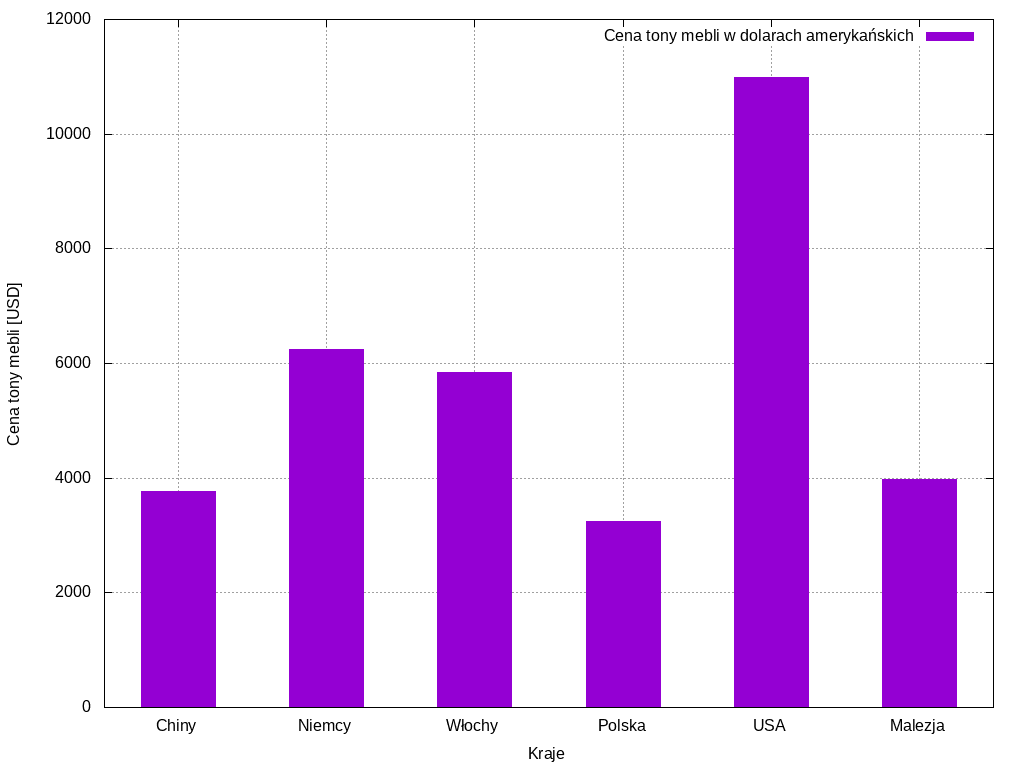
\includegraphics[scale=0.45]{price_weight}
				\caption{Wykres przedstawiający cenę za tonę mebli w danym państwie}
			\end{figure}
		
		\subsection{Uzasadnienie wyboru branży}
			\par Rynek e-commerce w Polsce z roku na rok notuje coraz lepsze wyniki. Według badań przeprowadzonych przez Gemius, prawie połowa Polaków robi zakupy przez internet. W ich opinii zakupy on-line są wygodniejsze, tańsze, dostępne całą dobę, dają możliwość większego wyboru produktów. Wedle informacji zawartych w sprawozdaniu "Handel internetowy w Polsce 2015, analiza prognoza rozwoju rynku e-commerce  na lata 2015-2020", e-handel notuje stabilną dynamikę wzrostu, niezależnie od sytuacji na całym rynku detalicznym.
			Polska jest również jednym z największych na świecie eksporterów mebli, a polska branża meblarska notuje zyski rok po roku, zarówno na rynku internetowym jak i stacjonarnym. Polscy producenci posiadają dobrą renomę  na rynkach eksportowych. Według analizy B+R Studio i Ogólnopolskiej Izby Gospodarczej Producentów Mebli, eksport polskich mebli w 2016 roku przekroczył 40 mld złotych. Rokrocznie wzrasta na poziomie 10 procent. Polskie produkty są cenione nie tylko za konkurencyjne ceny, ale również za solidne wykonanie, użyte materiały i design. 
		
			\begin{figure}[H]
				\centering
				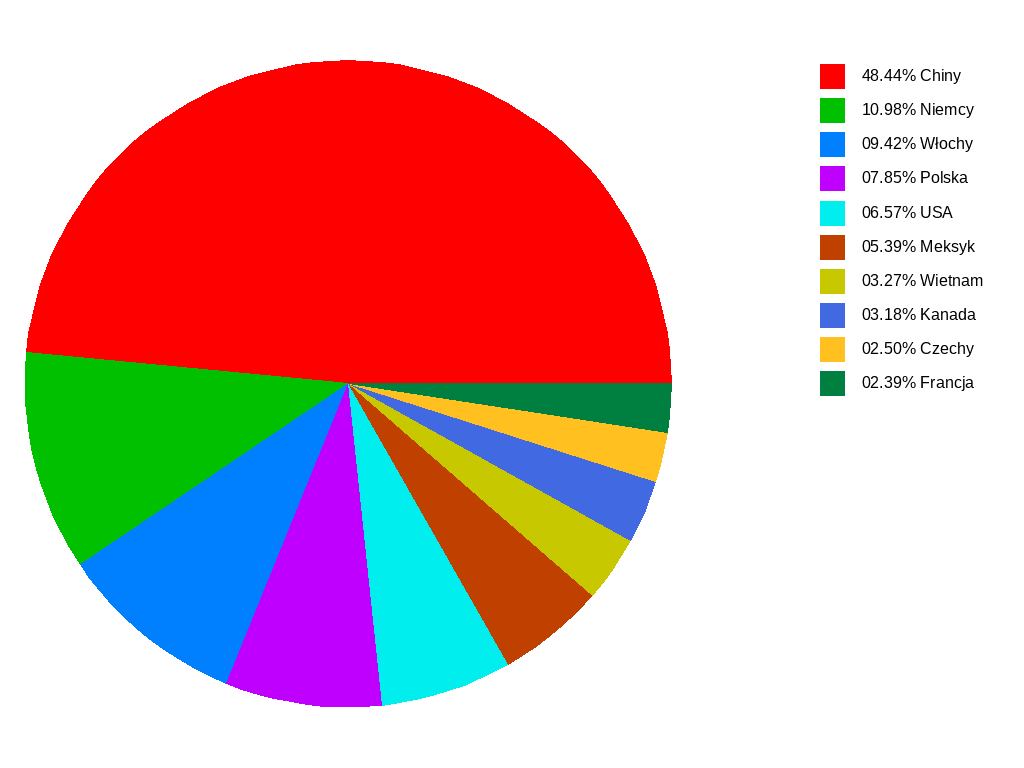
\includegraphics[scale=0.5]{export_swiat}
				\caption{Wykres przedstawiający procentowy udział czołowych krajów w rynku eksportowym}
			\end{figure}
	
		\subsection{Motywacje osobiste}
			\par Nadrzędną motywacją, która skłoniła mnie do próby podjęcia tego przedsięwzięcia, jest moje długoletnie doświadczenie w handlu i sukcesy z nią związane. Do tej pory działałam na rynku polskim, a jako osoba ambitna, chcę również sprawdzić swoje możliwości w handlu międzynarodowym. Dlatego też od dłuższego czasu obserwowałam skale sprzedaży na rynkach e-commerce. Ze względu na doświadczenie zawodowe i wykształcenie, posiadam obszerną wiedzę dotyczącą handlu jak i komunikacji społecznej. Dlatego wiem, że kluczową sprawą jest nie tylko bezpieczeństwo danych klientów, świetnie przygotowany sklep internetowy, ale również profesjonalna obsługa klienta
			\par Znaczącą motywacją było również pojawienie się kompleksowej umowy handlowo-gospodarczej "CETA", która usuwa konieczność opłacenia ceł, co upraszcza formalności i obniża koszty eksportu. 

	\section{Stan przygotowań do podjęcia działalności gospodarczej}
		\par W związku z planowanym przedsięwzięciem, podjęłam szereg działań umożliwiających mi szybsze rozpoczęcie pracy nad własnym sklepem. Na dzień dzisiejszy posiadam wiele narzędzi niezbędnych do działania sklepu internetowego. Są to kosztowne narzędzia programowe gwarantujące przede wszystkim niezależność, bezpieczeństwo sklepu jak i klientów, oraz nienaganne działanie platformy.

		\subsection{Posiadane środki}
			\paragraph{Organizacja firmy}
				\begin{itemize}
					\item Opracowany logotyp
					\item Zakupione domeny
						\begin{itemize}
							\item sklep-meblowy.org
							\item furniture-store.ca
						\end{itemize}
					\item oprogramowanie sklepu internetowego bazujące na platformie Drupal
						\begin{itemize}
							\item Tworzenie kont indywidualnych dla klientów;
							\item Tworzenie profili biznesowych dla kontrahentów;
							\item Dodawanie produktów ze zdjęciami;
							\item Wielojęzyczność;
							\item Przeliczanie walut;
							\item Przyjazny interfejs wraz z możliwością edycji;
							\item Integracja z portalami społecznościowymi;
							\item Statystyki odwiedzin;
							\item Rozbudowana wyszukiwarka produktów;
							\item Kategoryzacja produktów na podstawie wyszukiwanych pozycji;
							\item Synchronizacja z systemem ERP;
							\item Ochrona przed spamem;
						\end{itemize}
					\item oprogramowanie serwera stron internetowych
						\begin{itemize}
							\item Obsługa strony internetowej; 
							\item Obsługa kopii strony. 
						\end{itemize}
					\item oprogramowanie serwera wiadomości e-mail
						\begin{itemize}
							\item Podpisywanie poczty wychodzącej;
							\item Wysyłanie załączników;
							\item Skanowanie antywirusowe;
							\item Filtrowanie spamu.
						\end{itemize}
					\item centrala telefoniczna PBX
						\begin{itemize}
							\item Nagrywanie rozmów
							\item Obsługa polskiego i kanadyjskiego numeru
							\item Przekierowywanie rozmów
						\end{itemize}
					\item system zarządzania bazujący na platformie Redmine
						\begin{itemize}
							\item Przechowywanie danych klientów, kontrahentów, dostawców;
							\item Tworzenie projektów, grafików pracy;
							\item Obsługa sprzedaży;
							\item Obsługa zakupów;
							\item Kontrola stanów magazynowych;
							\item Obsługa wielu magazynów;
							\item Generowanie sprawozdań finansowych, deklaracji VAT itp.;
							\item Obsługa zarządzania produkcją;
							\item Zarządzanie środkami trwałymi.
						\end{itemize}
			\end{itemize}

			\section{Struktura organizacyjna}	
				\subsection{Wstęp}
			\par Wykorzystanie systemu zarządzania i sklepu internetowego zapewnia ciągłość i bezpieczeństwo obiegu informacji. Wprowadza także sformalizowany sposób organizacji i zarządzania przedsiębiorstwem. Formalizacja ta zachodzi na polu organizacji procesów zamówienia i reklamacji. Systemowe podejście do tych procesów pozwala na śledzenie kondycji i planowanie działań przedsiębiorstwa.
			
		\subsection{Proces zamówienia}  
			\par Aby zorganizować proces zamówienia należy zachować dotyczące go dane celem późniejszego ich przetwarzania i kontroli jakości produktu. Podstawowymi danymi do zapamiętania będzie tu data wpłynięcia zamówienia, oraz data jego realizacji. Proces zamówienia składa się z dwóch pod procesów. Są nimi proces produkcji i logistyki.
			
			\par Dając klientowi możliwość wyboru opcji wykończenia danego produktu musimy zapisać wybrane przez niego opcje celem przekazania jednoznacznego zlecenia produkcji, możliwości kontroli poprodukcyjnej, oraz prawidłowego zabezpieczenia wysyłki. Dane te należy przekazać również na adres e-mail klienta. Negatywne zdarzenia, na jakie należy być przygotowanym to roszczenia klienta o niezgodność towaru, uszkodzenie w transporcie, kontrola skarbowa. Organizacja procesu sprzedaży w opisany sposób eliminuje konieczność posiadania magazynu. Zamówiony towar wyprodukowany wedle specyfikacji klienta zostaje do niego dostarczony z pominięciem magazynowania.
			
			\subsubsection{Produkcja}
				Organizacja produkcji. Dane do zabezpieczenia:
				\begin{itemize}
					\item Opcje wybrane przez klienta 
					\item Zlecenie produkcji wraz z terminami
					\item Zdjęcia po produkcyjne przed i po pakowaniu
				\end{itemize}
				
			\subsubsection{Transport}
				Organizacja transportu. Dane do zabezpieczenia:
				\begin{itemize}
					\item Sposób i terminy dostawy
					\item Dokumenty SAD w przypadku eksportu
				\end{itemize}
			
			\subsubsection{Przebieg procesu}
				\par Przebieg procesu zamówienia przestawia poniższy schemat blokowy. Zostały na nim uwzględnione czynności, jakie należy wykonać w odpowiedniej kolejności wraz z dokumentami, jakie należy wystawić i ich oczekiwać celem prawidłowego wykonania procesu zamówienia oraz uniknięcia konsekwencji prawnych.
			
				\begin{figure}[H]
					\centering
					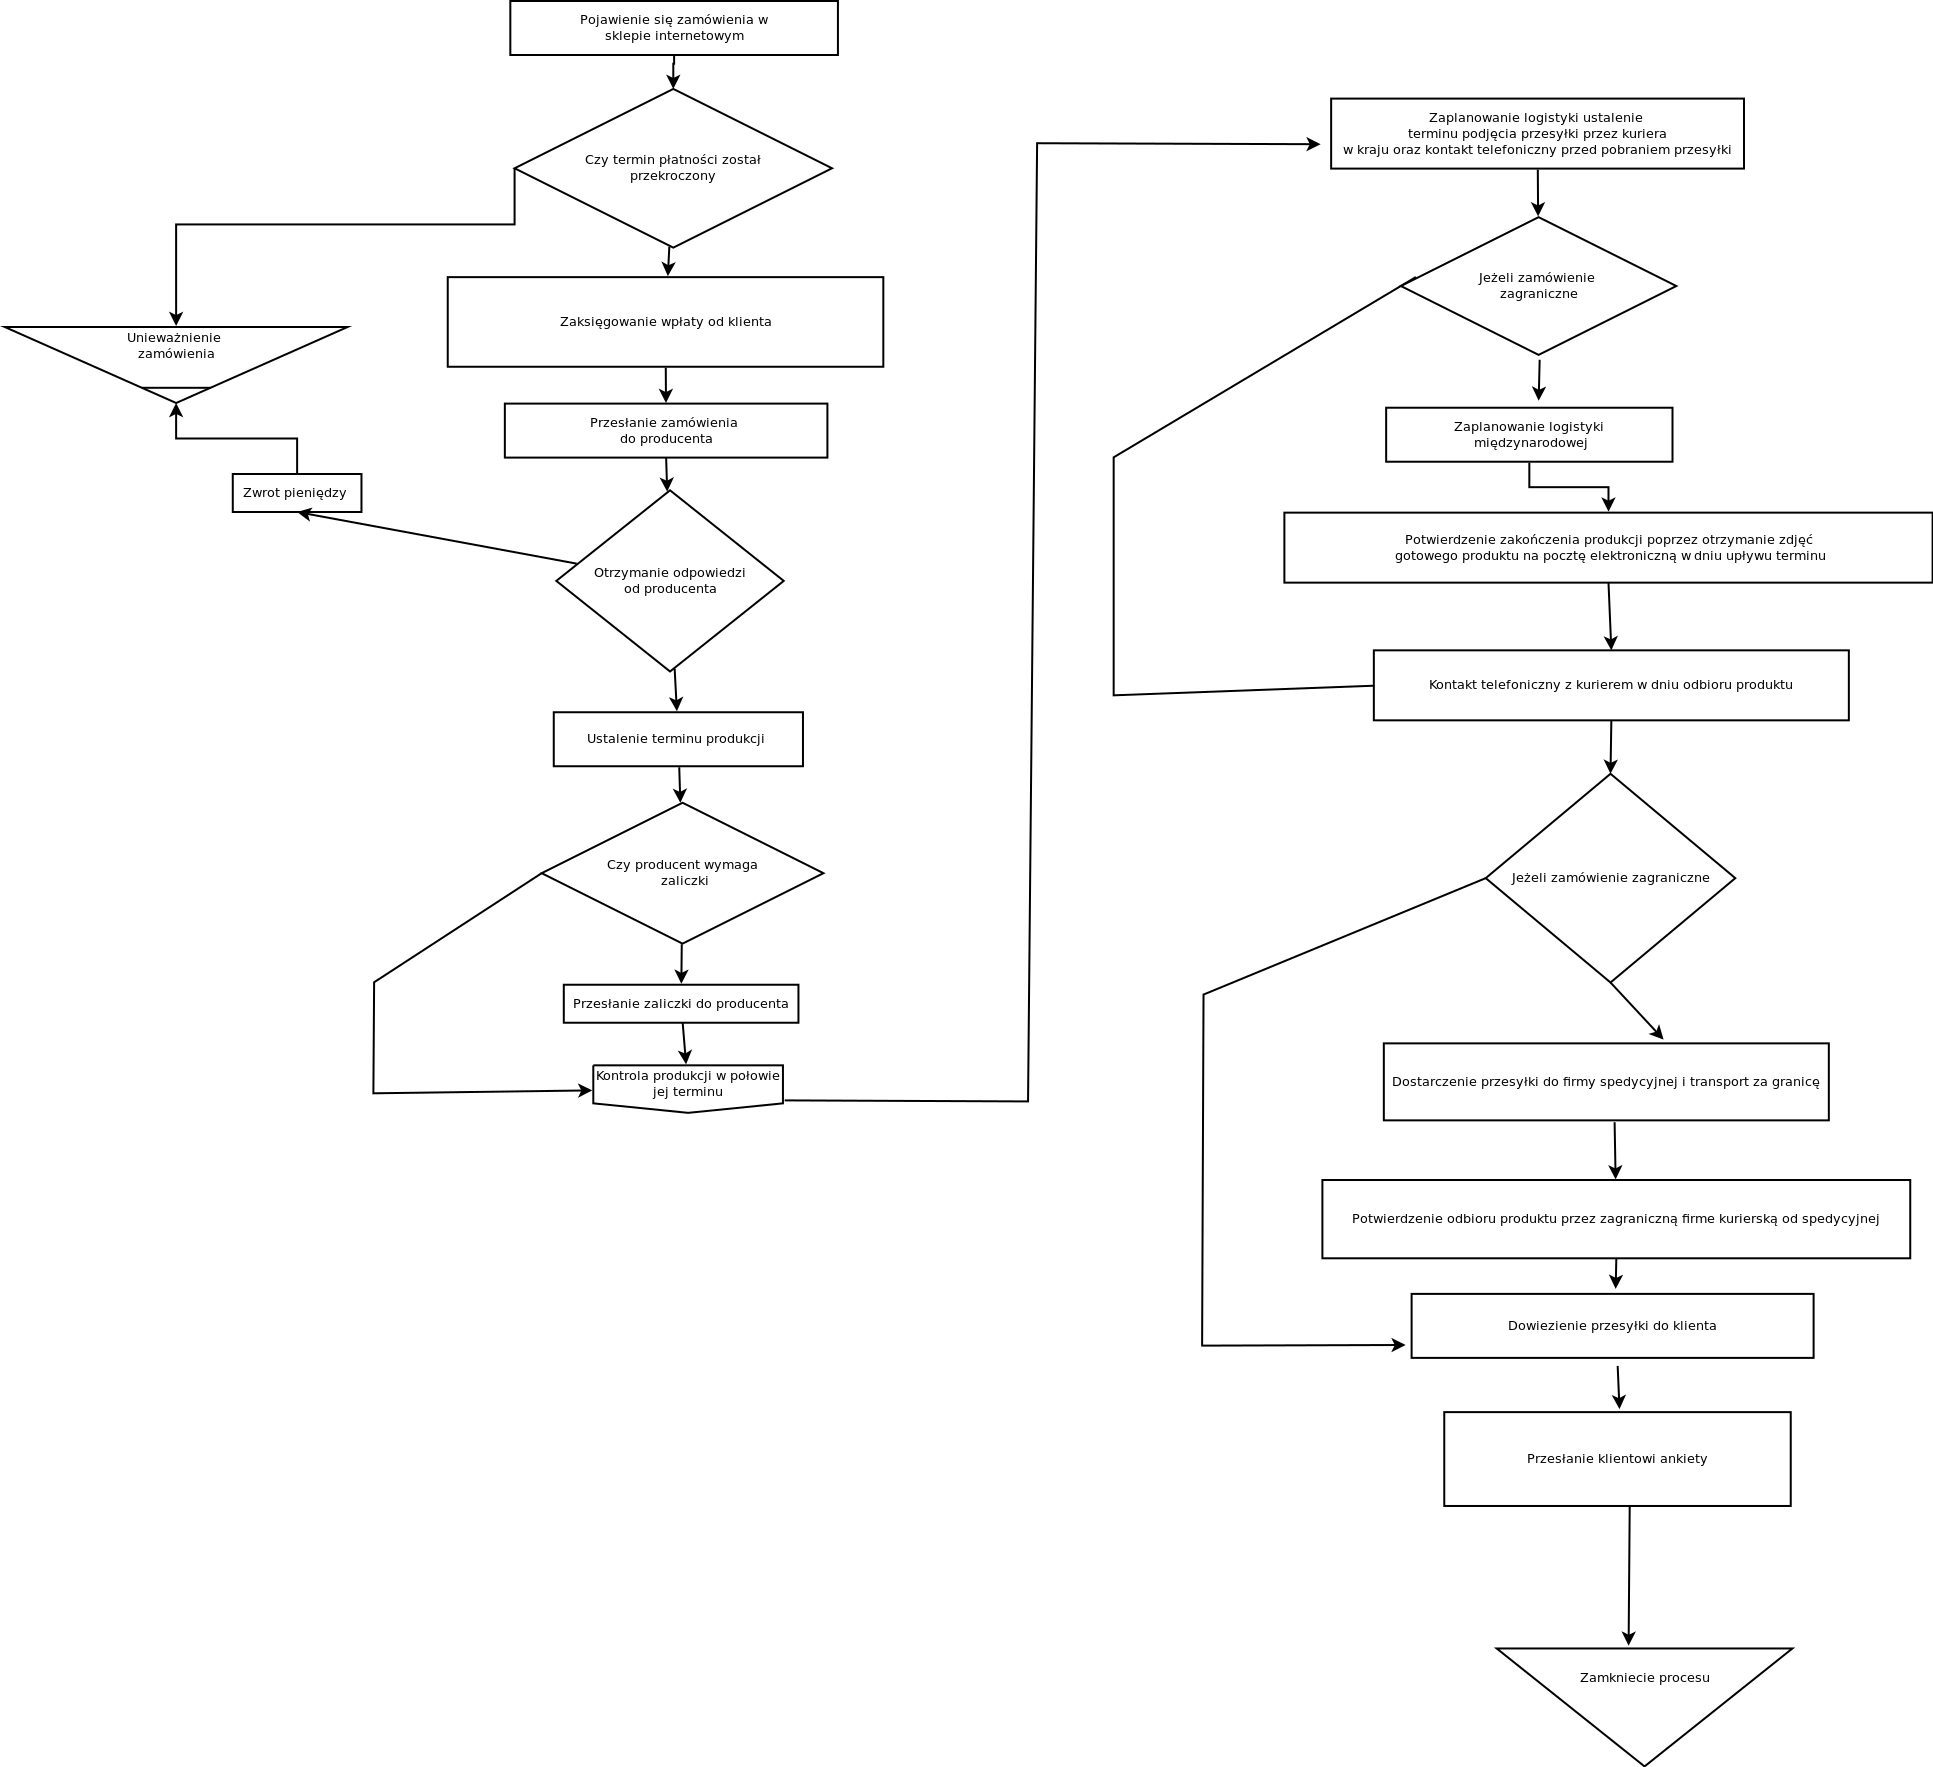
\includegraphics[scale=0.25]{zamowienie}
					\caption{Schemat procesu zamówienia}
				\end{figure}
			
		\subsection{Proces reklamacji}
			\par W tym procesie należy zabezpieczyć dane dotyczące zgłoszenia reklamacji, w skład których muszą wchodzić zdjęcia przedmiotu przesłane przez klienta w zgłoszeniu reklamacji. Na ich podstawie należy podjąć decyzję o uznaniu reklamacji lub odmowie. W wypadku uznania reklamacji i sprzedaży zagranicznej trzeba podjąć odpowiednią procedurę naprawy w kraju docelowym lub wysyłki nowego towaru z Polski i utylizacji uszkodzonego. W wypadku sprzedaży krajowej można zwrócić produkt do producenta celem usunięcia wad.
			
			
			\begin{figure}[H]
				\centering
				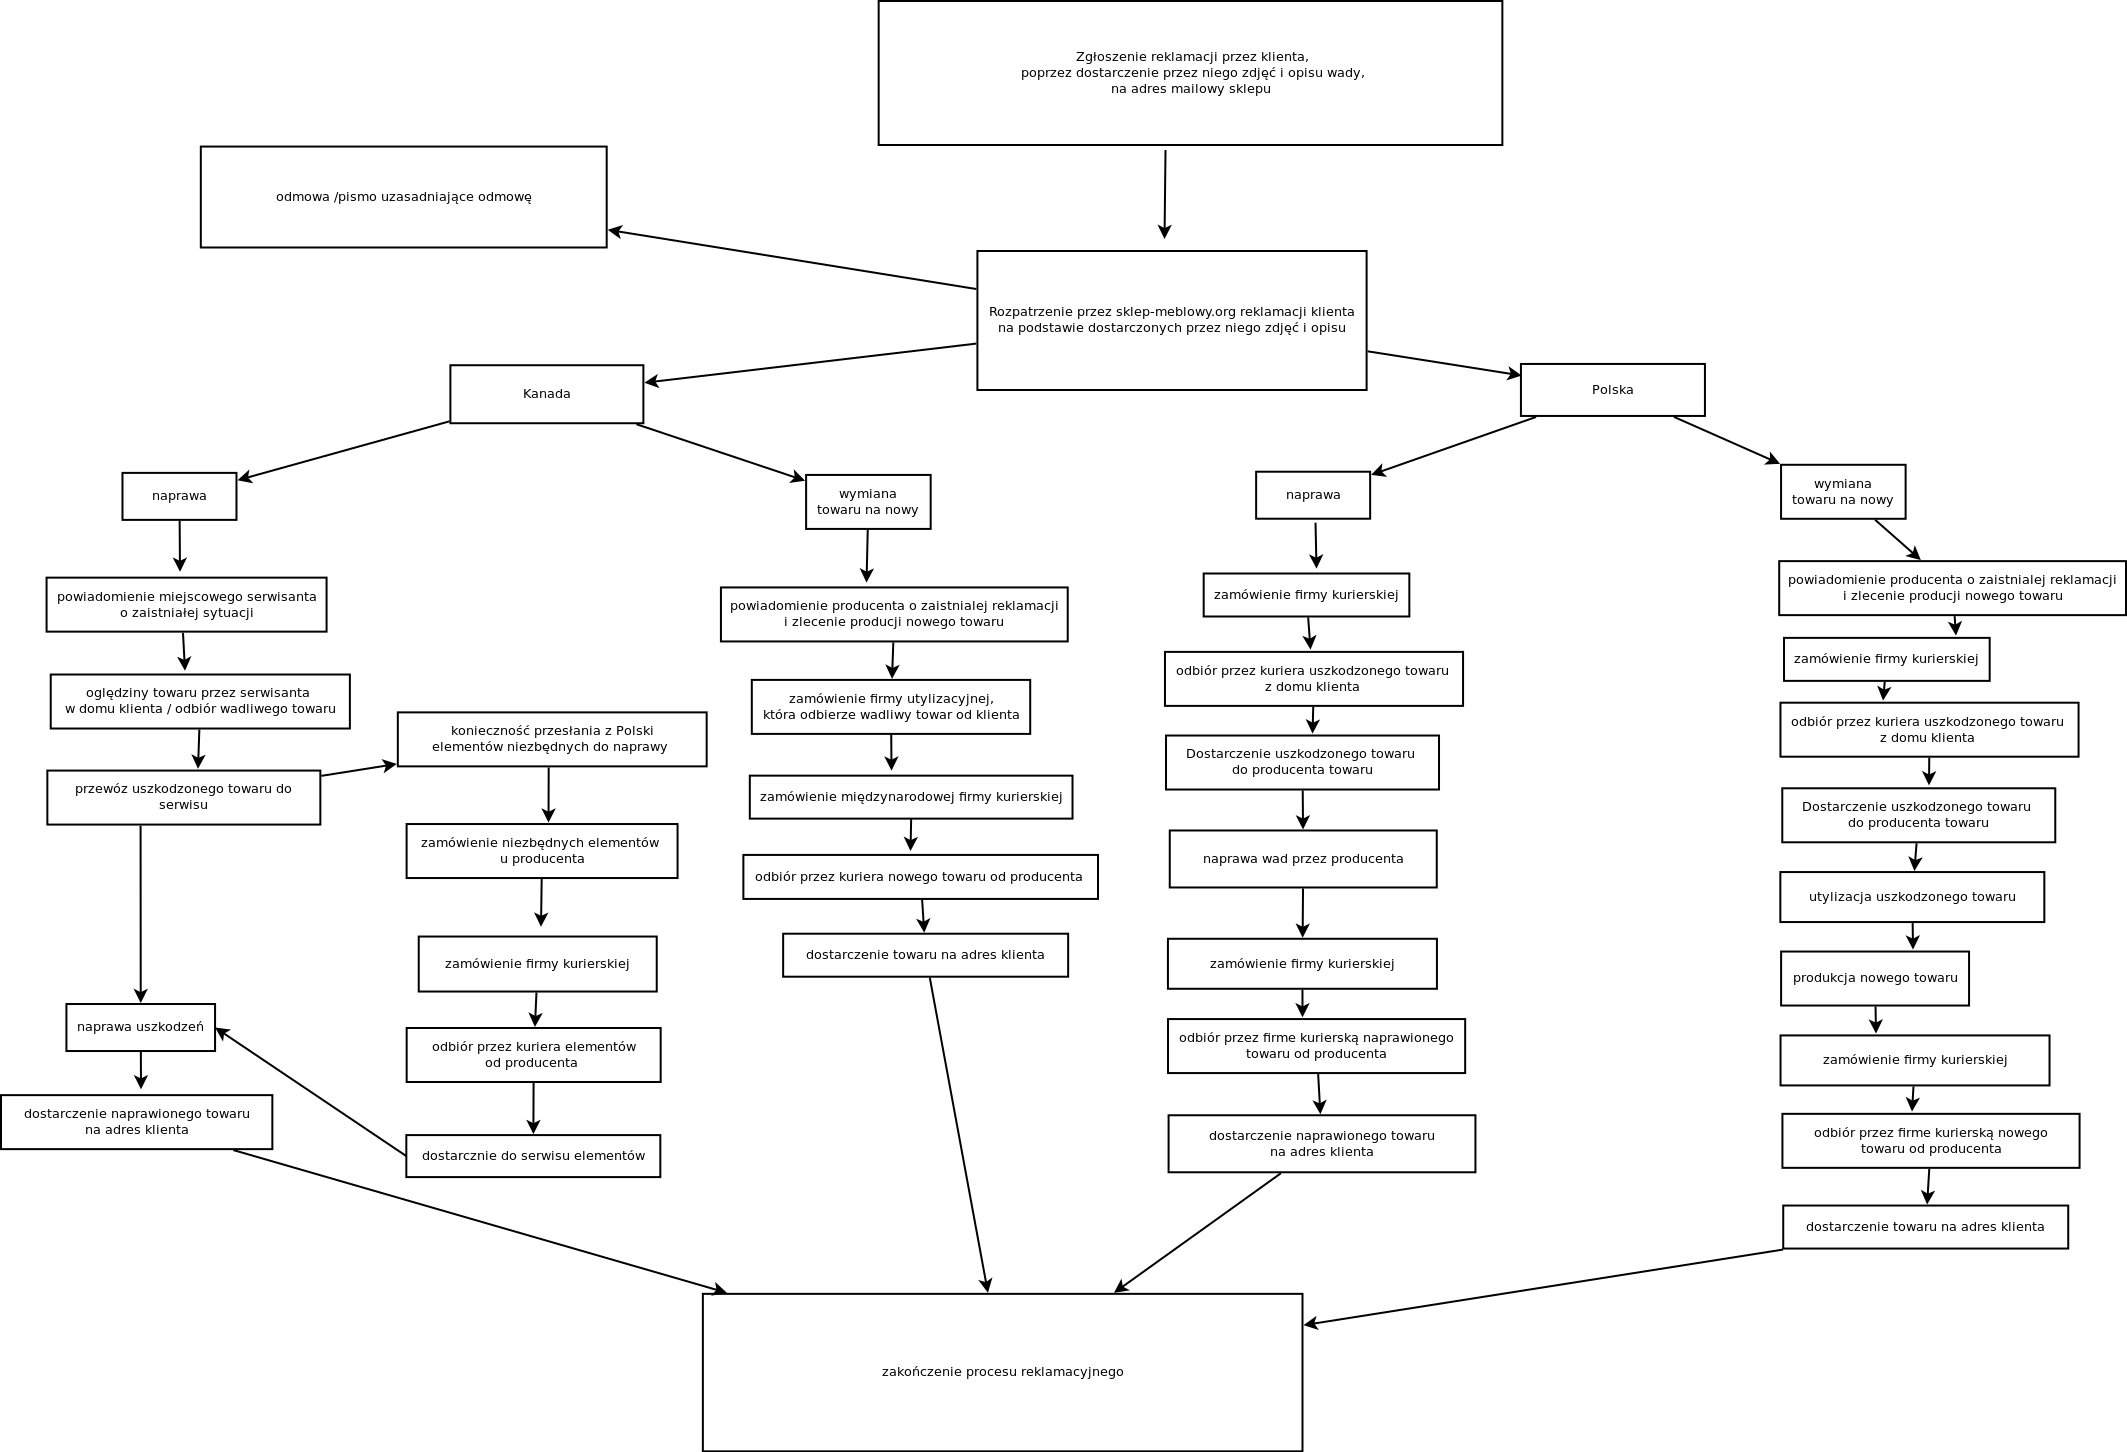
\includegraphics[scale=0.25]{reklamacja}
				\caption{Schemat procesu reklamacji}
			\end{figure}
			

			
			\section{Struktura zatrudnienia i wynagrodzeń}
		\subsection{Opis}
			\par W pierwszym roku prowadzenia działalności mojej firmy będę jej jedynym pracownikiem. Będę odpowiedzialna za pozyskiwanie producentów, których produkty będą prezentowane na stronie, obsługą klientów, logistyką oraz będę się zajmować innymi działaniami niezbędnymi do prowadzenia sklepu internetowego. W trakcie rozwoju firmy planuję zatrudnienie pracowników, którzy przejmą ode mnie część obowiązków. Wprowadzając awanse pionowe, oznaczające pięcie się "w górę" na coraz to wyższe stanowiska w firmie, w drugim roku handlowiec awansuje na stanowisko starszego handlowca, robiąc tym samym lukę, co pozwala na zatrudnienie nowej osoby na stanowisko handlowca. Powielając ten schemat w trzecim roku, starszy handlowiec awansuje na stanowisko kierownika; handlowiec zostanie starszym handlowcem. W ten sposób można zatrudnić kolejną osobę, która zapełni lukę w hierarchii organizacyjnej przedsiębiorstwa. 
			 
			
			\begin{figure}[H]
				\centering
				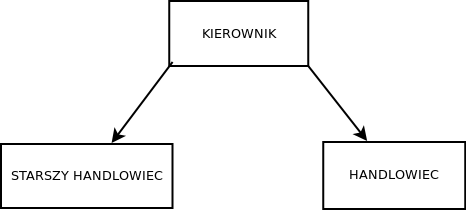
\includegraphics[scale=0.5]{struktura_org}
				\caption{Struktura organizacyjna przedsiębiorstwa}
				\label{search_pl}
			\end{figure}
			
			
		\subsubsection{Opis stanowisk pracy}
			\par Handlowiec
				\begin{itemize}
					\item telefoniczna i mailowa obsługa klienta
					\item obsługa zamówień 
					\item umieszczanie postów na portalach społecznościowych
					\item prowadzenie sprzedaży internetowej poprzez portale aukcyjne
					\item kompletowanie zamówień
			   	\end{itemize}
			
			\par Starszy handlowiec
				\begin{itemize}
					\item umieszczanie nowych produktów na stronie internetowej
					\item sporządzanie szczegółowych opisów produktów
					\item wystawianie faktur, paragonów
					\item kontakt z producentami
					\item kontrola procesu produkcji 
					\item organizowanie logistyki
				\end{itemize}	
					
			\par Kierownik
				\begin{itemize}
					\item pozyskiwanie nowych producentów mebli
					\item kreowanie oraz implementacja rozwiązań, które usprawnią sprzedaż internetową
					\item monitorowanie pracy handlowca i starszego handlowca
					\item monitorowanie rynku i konkurencji
					\item rozpatrywanie reklamacji
					\item delegowanie zadań podległym sobie pracownikom
				\end{itemize}

				
		\subsubsection{Wynagrodzenia}
			\par Przez "wynagrodzenie" rozumiemy ekwiwalent należny za pracę pracownika na rzecz pracodawcy w ramach stosunku pracy. W trakcie rozwoju firmy mam zamiar zatrudniać pracowników na postawie umowy o pracę. Wynagrodzenie początkowe jakie będzie otrzymywał pracownik, to wynagrodzenie minimalne, które zostało ujęte w kodeksie pracy. Na dzień dzisiejszy wynosi ono 2000 zł. brutto. Po otrzymanym awansie, pracownik będzie otrzymywał coraz wyższe wynagrodzenie adekwatne do zajmowanego stanowiska. Można przyjąć, iż będą to podwyżki na poziomie 20-30 \%.
			
			\par Jak powszechnie wiadomo wynagrodzenie pracownika pełni nie tylko funkcję czysto dochodową. Również bardzo ważną jest tu funkcja motywacyjna- im większy wpływ na swoją płacę ma pracownik, tym większą ma motywację do pracy. Dlatego bardzo ważne jest wprowadzenie systemu premii, nagród itp.. W moim przypadku może być to premia związana ze wzrostem sprzedaży, sumienności wykonywanych obowiązków, czy też zaangażowania w rozwój sklepu.



	\chapter{Analiza rynku, plan marketingowy}
		\section{Charakterystyka rynku}
	\par Należy tu scharakteryzować dwa rynki. Jednym z nich jest rynek polski, z którego to czerpane będą produkty oraz prowadzona będzie na nim sprzedaż dla klientów rodzimych. Drugim jest rynek kanadyjski, który będzie celem eksportu.

	\subsection{Rynek polski}
		\par Według badań przeprowadzonych przez Millward Brown,  rynek polski składa się 38.5 mln mieszkańców, z których 25.8 mln to internauci. 48\% z nich dokonało zakupów za pośrednictwem sklepów internetowych - daje to potencjalną grupę nabywców ok. 12 mln osób.  Jako, że statystycznie w Polsce mamy 14.1 mln. gospodarstw domowych, a 76\% z nich ma dostęp do internetu, to te 12 mln. potencjalnych nabywców mieszka w 10 mln. gospodarstw domowych. Średnia ilość internautów na gospodarstwo domowe 1.2. Jednocześnie rozwój branży mieszkaniowej sugeruje również wzrost na rodzimym rynku mebli. W pierwszym kwartale 2016 roku rozpoczęto budowę 133 tys. mieszkań, a branża odnotowała prawie 4\% wzrost.

		\begin{table}[H]
			\centering
			\begin{tabular}{|l|l|l|l|}
			\hline
																															& Miasto   & Wieś     & Razem    \\ \hline
			\begin{tabular}[c]{@{}l@{}}Liczba gospodarstw \\ domowych\end{tabular}               & 9400000  & 4700000  & 14100000 \\ \hline
			\begin{tabular}[c]{@{}l@{}}Liczba osób w gospodarstwach \\ domowych\end{tabular}     & 22842000 & 15322000 & 38164000 \\ \hline
			\begin{tabular}[c]{@{}l@{}}Średnia liczba osób\\ na gospodarstwo domowe\end{tabular} & 2.43     & 3.26     & 2.71     \\ \hline
			\end{tabular}
			\caption{Tabela dane dotyczące zamieszkania w Polsce}
			\label{avg_home_pl}
		\end{table}
	
		\par Rynek e-commerce w Polsce z roku na rok notuje coraz lepsze wyniki. Według badań przeprowadzonych przez Gemius, prawie połowa Polaków robi zakupy przez internet. W ich opinii zakupy on-line są wygodniejsze, tańsze, dostępne całą dobę i dają możliwość większego wyboru produktów. Wedle informacji zawartych w sprawozdaniu "Handel internetowy w Polsce 2015, analiza prognoza rozwoju rynku e-commerce  na lata 2015-2020", e-handel notuje stabilną dynamikę wzrostu, niezależnie od sytuacji na całym rynku detalicznym.
		
	
		\begin{figure}[H]
			\centering
			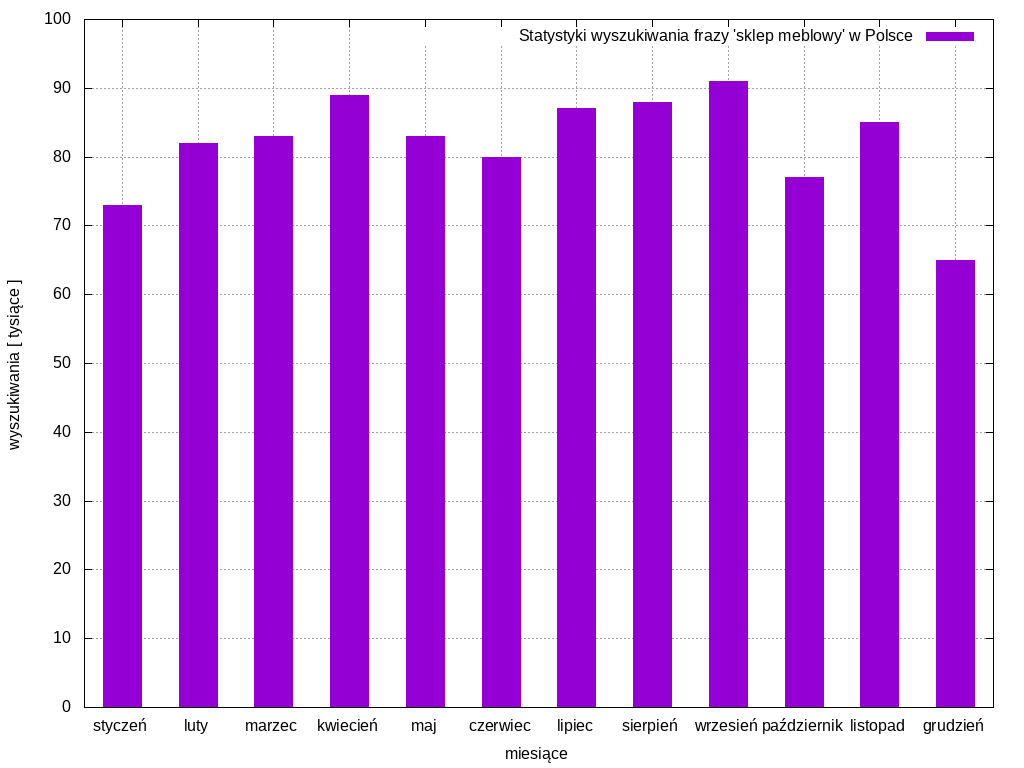
\includegraphics[scale=0.5]{stat_wysz_polska}
			\caption{Statystyki wyszukiwania frazy 'sklep meblowy' w Polsce}
			\label{search_pl}
		\end{figure}
	 
		\par Każdego miesiąca wedle statystyk "Google" w Polsce notowanych jest około 78 tyś. wyszukiwań frazy "sklep meblowy". Ludzie Ci to potencjalni klienci. Daje to sumarycznie prawie 1 mln. wyszukiwań rocznie. Na samym tylko "allegro.pl" korzystając z danych z ich magazynu, sprzedawanych jest dziennie ok. 2,5 tys. mebli dziennie. Biorąc pod uwagę, że według danych GUS mali producenci mebli (tzn. nie zatrudniający więcej jak 9 osób), posiadają  około 9\% całego polskiego rynku sprzedaży wewnętrznej. Daje to pule 90 tyś. klientów dla małych producentów mebli. Biorąc pod uwagę ilość małych producentów, według danych z 2010 roku około 13 tys. podmiotów daje około 6 klientów na podmiot. Zakładając średnią dla handlu internetowego w Polsce konwersję na 15\%,  aby uzyskać taką liczbę klientów należy ściągnąć na nią średnio 400 osób rocznie. Czyli 1.1 osoby dziennie, z czego 20\% stanowią meble do sypialni, 5\% stanowią meble kuchenne, a 75\% do salonów i jadalni.
		Bardziej szczegółowe dane prezentuje wykres.
	
	\subsection{Rynek kanadyjski}
		\par Rynek kanadyjski składa się z 31 mln. mieszkańców, z których 90\% tj. 27.9 mln. ludzi to internauci. Z handlu internetowego korzysta 51\% użytkowników, jest to ok. 14.3 mln. potencjalnych nabywców, z czego 34\% poszukuje w internecie mebli. Kanada liczy sobie 12.5 mln. gospodarstw domowych a średnia ilość ludzi w gospodarstwie wynosi 2.5.  Wynika z tego, że rynek stanowi 4.9 mln. użytkowników mieszkających w 1.96 mln. gospodarstw domowych. 

		\begin{table}[H]
		\centering
		\resizebox{\textwidth}{!}{%
		\begin{tabular}{|l|l|l|l|l|l|}
		\hline
																														& Domy jednorodzinne & \begin{tabular}[c]{@{}l@{}}Budynki apartamentowe \\ (powyżej 5 kondygnacji)\end{tabular} & Mieszkania ruchome & Inne    & Razem    \\ \hline
		\begin{tabular}[c]{@{}l@{}}Liczba gospodarstw\\ domowych\end{tabular}                 & 6871315            & 1114925                                                                                  & 163515             & 4285760 & 12435520 \\ \hline
		\begin{tabular}[c]{@{}l@{}}Liczba osób w \\ gospodarstwach domowych\end{tabular}      & 19310825           & 2030040                                                                                  & 365585             & 9365975 & 31072420 \\ \hline
		\begin{tabular}[c]{@{}l@{}}Średnia liczba osób \\ na gospodarstwo domowe\end{tabular} & 2.8                & 1.8                                                                                      & 2.2                & 2.2     & 2.5      \\ \hline
		\end{tabular}%
		}
		\caption{Dane statystyczne dotyczące zamieszkania w Kanadzie}
		\label{avg_home_ca}
		\end{table}

		\par Każdego miesiąca wedle statystyk "google" dla Kanady, fraza 'furniture store' wyszukiwana jest ok. 1 mln. przez unikalnych użytkowników. Są to użytkownicy poszukujący sklepów z meblami. Statystyka ta nie uwzględnia użytkowników korzystających z portali aukcyjnych. Na podstawie pozyskanych informacji, udało się ustalić, że 3.9 mln. użytkowników korzysta z portali aukcyjnych lub znanych stron przy zakupie mebli, a ok. 1 mln. klientów poszukuje nowych sklepów. Jednocześnie ze statystyk wynika, że udział polskich producentów w eksporcie produktów meblowych do Kanady wynosi 1.5\%. Daje to całkowitą pulę klientów 73.5 tyś. osób rocznie. Z braku danych statystycznych dla Kanady, przyjmijmy tu udział w rynku dla małych producentów podobny jak na rynku rodzimym tj. 9\%. Daje to 6.6 tyś. klientów rocznie. Rozkładając to na małych polskich producentów mebli, których jest 13.5 tyś. zakładając, (również z braku danych), że 25\% małych producentów eksportuje meble do Kanady daje to 1.95 klienta na podmiot rocznie. Aby osiągnąć nawet tak znikomą sprzedaż przy współczynniku konwersji 15\%, należy przyciągnąć do sklepu internetowego 13 unikalnych kanadyjskich użytkowników rocznie.
		
		\begin{figure}[H]
			\centering
			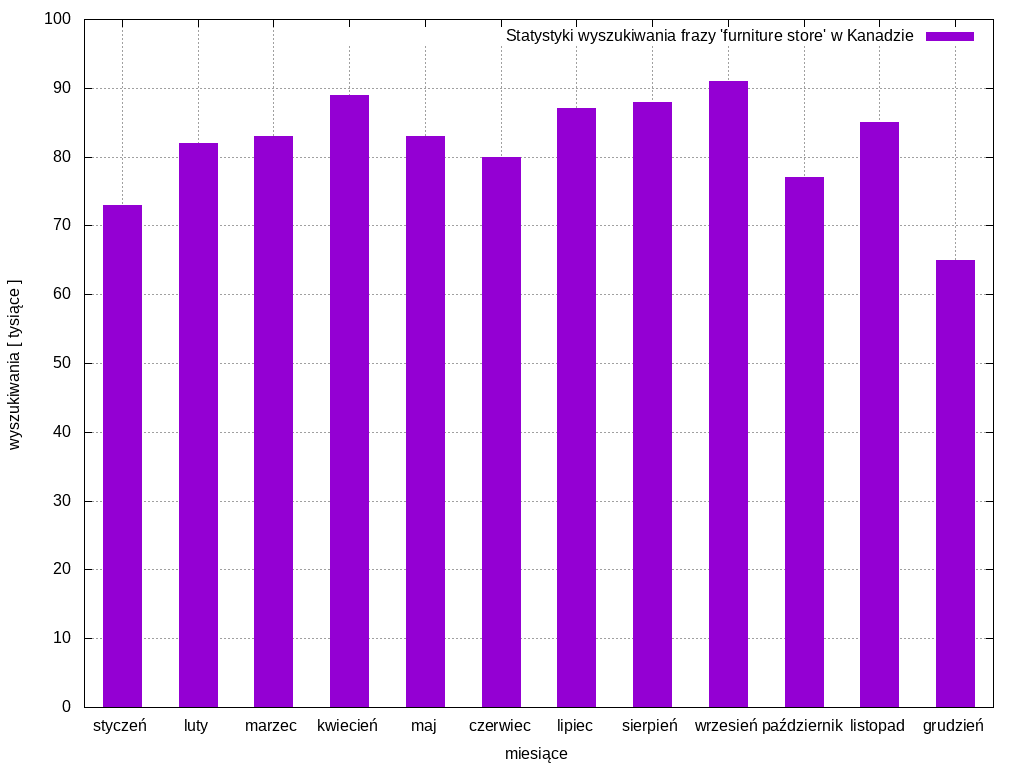
\includegraphics[scale=0.5]{stat_wysz_kanada}
			\caption{Statystyki wyszukiwania frazy 'furniture store' w Kanadzie}
		\end{figure}
	
	
	\section{Charakterystyka klientów}
		\subsection{Klienci indywidualani}
			\par Nabywcami w moim sklepie internetowym, będą oczywiście użytkownicy internetu. Należy ich podzielić na dwie kategorie: klientów polskich i klientów kanadyjskich.
			Według badań przeprowadzonych przez Millward Brown , w Polsce z internetu korzysta 76 procent obywateli, z czego 48 procent deklaruje, że chociaż raz w życiu dokonało zakupu za pośrednictwem internetu. W 2016 roku największą ilość nabywców na rynku e-commerce stanowiły osoby młode w wieku 25-35 lat, z wykształceniem średnim lub wyższym . To właśnie do nich będę przede wszystkim kierować swoją ofertę. Są to najczęściej osoby zabiegane ,które na co dzień  nie mają czasu na odwiedzanie sklepów stacjonarnych. Nabywców, którzy cenią sobie wysoką jakość produktu, jego oryginalność i niepowtarzalność.
			
			\par Osoby robiące zakupy online w powodach korzystania z tego rodzaju rozwiązania podają wygodę, oszczędność czasu i pieniędzy oraz większy wybór dostępnych produktów. Jako motywacje - 84\% podało dostępność całą dobę, 79\% brak konieczności jechania do sklepu, 75\% ceny atrakcyjniejsze niż w sklepach stacjonarnych. Dużym atutem była również dogodna forma dostawy i zwrotów.
			
			\par Eksport polskich mebli do Kanady działa coraz prężniej. Z najnowszych badań wynika, że na 35 milionów mieszkańców Kanady, aż 90\% jest czynnymi użytkownikami internetu. Kanadyjczycy bardzo chętnie kupują nasze rodzime meble drewniane, ze szczególnym wyróżnieniem mebli sypialnianych  oraz foteli, krzeseł i mebli tapicerowanych. Według moich spostrzeżeń jakie nabyłam podczas badania tamtejszego rynku, Kanadyjczycy gustują w pikowanych, skórzanych sofach, drewnianych , zdobionych łóżkach, dużych ,rodzinnych stołach. Mają duże zamiłowanie do folklorystycznych wzorów, których nie wyprodukują im duże zakłady stolarskie. Przede wszystkim takie produkty będę kierować za ocean.
					
		
	\section{Oczekiwania i potrzeby klientów}
		\par Z doświadczenia życiowego wynika, że klienci oczekują zakupu jak najlepszego produktu w jak najkorzystniejszej cenie. Głównym kryterium jest tu jednak jakość materiałów. Tkaniny obiciowe muszą być dobrej jakości, elementy drewniane muszą być dobrze, równomiernie wybarwione, a półki nie wypaczać się z czasem. Ważne jest również nie używanie plastikowych uchwytów do sprężyn w meblach tapicerowanych wykorzystywanych przez producentów na potęgę ze względu na niskie koszty. Niestety degradują się one w bardzo krótkim czasie co powoduje tzw. wychodzenie sprężyn i zapadnięcie mebla. Niezbędna jest więc kontrola jakości i inspekcja wizualna wysyłanego towaru. Jak udało się ustalić klienci są w stanie zapłacić więcej za dobrze wykonany produkt. Żyjemy w czasach gdzie rynki są przepełnione produktami z masowej produkcji, które nie zadowalają części klientów. Społeczeństwo polskie jak i zagraniczne corocznie się wzbogaca, dając nam tym samym wielkie pole do działania. Również sklepom internetowym. Przy tym bardzo ważny jest czas realizacji zlecenia, który musi zostać zminimalizowany. Kolejnym bardzo istotnym czynnikiem jest wspomniana już wcześniej możliwość personalizacji produktu. Klient musi mieć możliwość wyboru tkanin, wybarwień, rodzajów drewna lub wymiarów mebla. Sklep internetowy musi wychodzić naprzeciw oczekiwaniom klienta i umożliwiać personalizację mebli poczynając od materiałów a kończąc na detalach takich jak: nóżki, okucia czy chociażby guziki.
		
		
	\section{Analiza rynku}
		\par Na potrzeby polityki cenowej przeprowadzona została wstępna analiza rynku obejmująca badanie statystyczne najpopularniejszych portali aukcyjnych w Polsce i Kanadzie. Przebadane portale to ebay.ca i allegro.pl. Metodyką przeprowadzonej analizy było zestawienie pięciu par podobnych między sobą artykułów, a następnie wyliczenie na tej podstawie średniej arytmetycznej. Na podstawie przeprowadzonej analizy udało się ustalić następujące ceny średnie artykułów z danych grup:
		
		\begin{table}[H]
		\centering
		\begin{tabular}{|l|l|l|}
		\hline
					& Polska [zł] & Kanada [zł]\\ \hline
		Komody 	& 384  & 2613 \\ \hline
		Fotele 	& 1058 & 2943 \\ \hline
		Sofy   	& 3729 & 9611 \\ \hline
		Stoły  	& 1185 & 3366 \\ \hline
		Łóżka  	& 1355 & 6145 \\ \hline
		\end{tabular}
		\caption{Średnia cena grup produktów w Polsce i Kanadzie}
		\label{avg_grp_price_ca_pl}
		\end{table}

		Ponadto dzięki powziętej analizie udało się wyliczyć średnią cenę towarów Polsce jak i w Kanadzie. Średnia cena w Polsce wynosi 1831 zł, a w Kanadzie 5516 zł. Co daje różnicę w cenie średniej w wysokości 3685 zł. Jest potencjalny zarobek w przypadku eksportu. Jednak dla określenia polityki cenowej istotne jest jeszcze określenie średniej ceny transportu towaru od producenta do klienta. Na tę potrzebę przeprowadzono analizę dokładnie tą samą metodologią. Jej wyniki prezentuję tabela poniżej.
		
		\begin{table}[H]
		\centering
		\begin{tabular}{|l|l|l|l|}
		\hline
					& Polska \textless-\textgreater Polska [zł] & Kanada \textless-\textgreater Kanada [zł] & Polska \textless-\textgreater Kanada [zł] \\ \hline
		Komody 	& 69                                 & 414                                & 960                                \\ \hline
		Fotele 	& 51                                 & 408                                & 960                                \\ \hline
		Sofy   	& 480                                & 1225                               & 1606                               \\ \hline
		Stoły  	& 94                                 & 1137                               & 960                                \\ \hline
		Łóżka  	& 321                               	& 1167                               & 1200                               \\ \hline
		\end{tabular}
		\caption{Średnia cena transportu wybranych grup produktów}
		\label{avg_grp_shp_price}
		\end{table}
		
		Dzięki tej analizie ustalono, że średnia cena wysyłki towaru w Polsce wynosi 203zł, cena wysyłki w Kanadzie wynosi 870zł, a przesyłki z Polski do Kanady 1137zł. Na tej podstawie można ustalić średnią kwotę wysyłki produktu z Polski do Kanady, na którą składać się będą wysyłka z Polski do Kanady oraz wysyłka na terenie Kanady. Nie wlicza się w nią natomiast cena transportu w Polsce, ponieważ wybrane firmy spedycyjne dysponują własną flotą na terenie Polski. Na tej podstawie średni koszt wysyłki oszacować można na 2007 zł.
		
		Na podstawie powyższych analiz można sformułować ogólny zarys cen obowiązujących na rynku, polskim średnia cena produktu 1831 zł, a średni koszt transportu 203zł. Natomiast dla rynku kanadyjskiego 5516 zł, średni koszt transportu to 870zł, oraz przedstawić poniższą tabelę zawierającą ceny średnie powiększone o średni koszt transportu.
		
		\begin{table}[H]
		\centering
		\begin{tabular}{|l|l|l|}
		\hline
					& Polska [zł]& Kanada [zł]\\ \hline
		Komody 	& 453  & 3027 \\ \hline
		Fotele 	& 1109 & 3351 \\ \hline
		Sofy   	& 4209 & 10836 \\ \hline
		Stoły  	& 1279 & 4503 \\ \hline
		Łóżka  	& 1676 & 7312 \\ \hline
		\end{tabular}
		\caption{Średnia cena produktu w Polsce i Kanadzie powiększona o średni koszt transportu}
		\label{avg_price_pl_ca}
		\end{table}

		Na podstawie powyższych można ustalić  następującą politykę cen dla Polski i dla Kanady. Korzystając z danych GUS o polskim rynku wewnętrznym można ustalić marżę na 20\%. Co do rynku kanadyjskiego do ustalenia marży konieczne będzie wykorzystanie informacji ustalonych podczas analizy rynkowej.
		
		\begin{figure}[H]
			\centering
			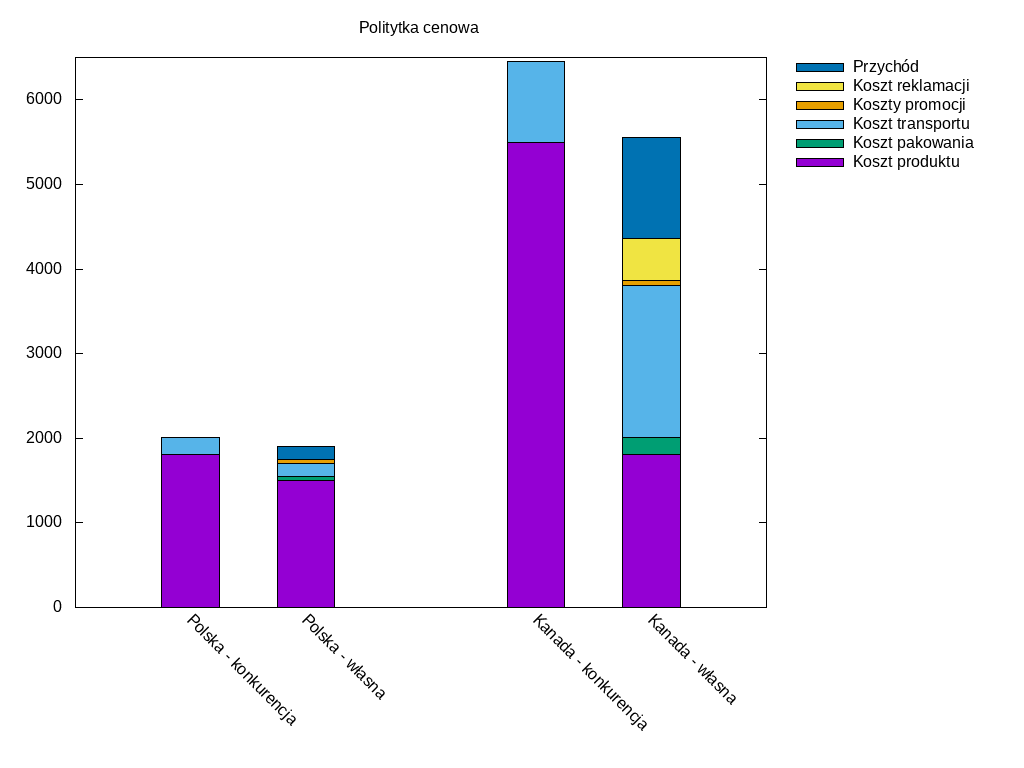
\includegraphics[scale=0.5]{polityka_cen}
			\caption{Polityka cenowa w Polsce i Kanadzie}
			\label{polityka_cen}
		\end{figure}

		W dziale charakterystyki rynku udało się ustalić średnią liczbę 6 klientów na producenta na rynku rodzimym, oraz średni przychód ze sprzedaży na 248 zł. Na rynku kanadyjskim natomiast średnią liczbę klientów na 1.95 klienta na podmiot. Biorąc pod uwagę dane z jednego producenta uzyskujemy przychód 1488 zł dla rynku polskiego. Dla rynku kanadyjskiego natomiast wyznaczono politykę cen na poziomie 80\% ceny konkurencji. Na podstawie ceny średniej w wysokości 5108 zł, udało się ustalić średni przychód w wysokości 910 zł. 

		\[ f(m) = (s_p \times p_p + s_k \times d_k ) \times m \]
		
		\begin{itemize}
			\item{\( s_p \)} średnia sprzedaż w Polsce na jednego producenta
			\item{\( d_p \)} średni dochód w Polsce ze sztuki sprzedanego towaru
			\item{\( s_k \)} średnia sprzedaż w Kanadzie na jednego producenta
			\item{\( d_k \)} średni dochód w Kanadzie ze sztuki sprzedanego towaru
			\item{m} liczba współpracujących producentów
		\end{itemize}
		
		Po podstawieniu parametrów i wyliczeniu otrzymujemy funkcję:
		
		\[	f(m) = 3262.5 \times m \]

		Wykres tej funkcji przedstawia przychód w zależności od ilości producentów przy założeniu osiągnięcia średniej sprzedaży.
		
		\begin{figure}
			\centering
			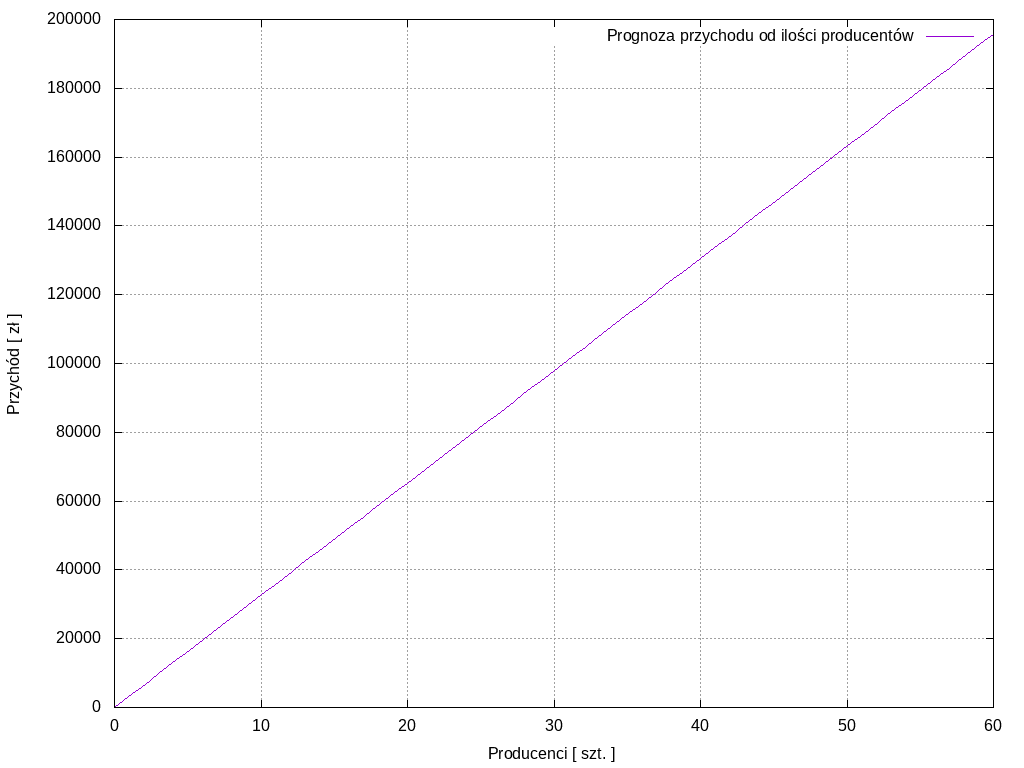
\includegraphics[scale=0.5]{income_prod}
			\caption{Wykres zależności przychodów od ilości producentów}
			\label{income_prod}
		\end{figure}

		Ważną informacją będzie też liczba odwiedzin potrzebna do osiągnięcia średniej sprzedaży. 
		
		\[ f(m) = \dfrac{ s_p + s_k }{w_k} \times m \] %konwersja
		
		\begin{figure}
			\centering
			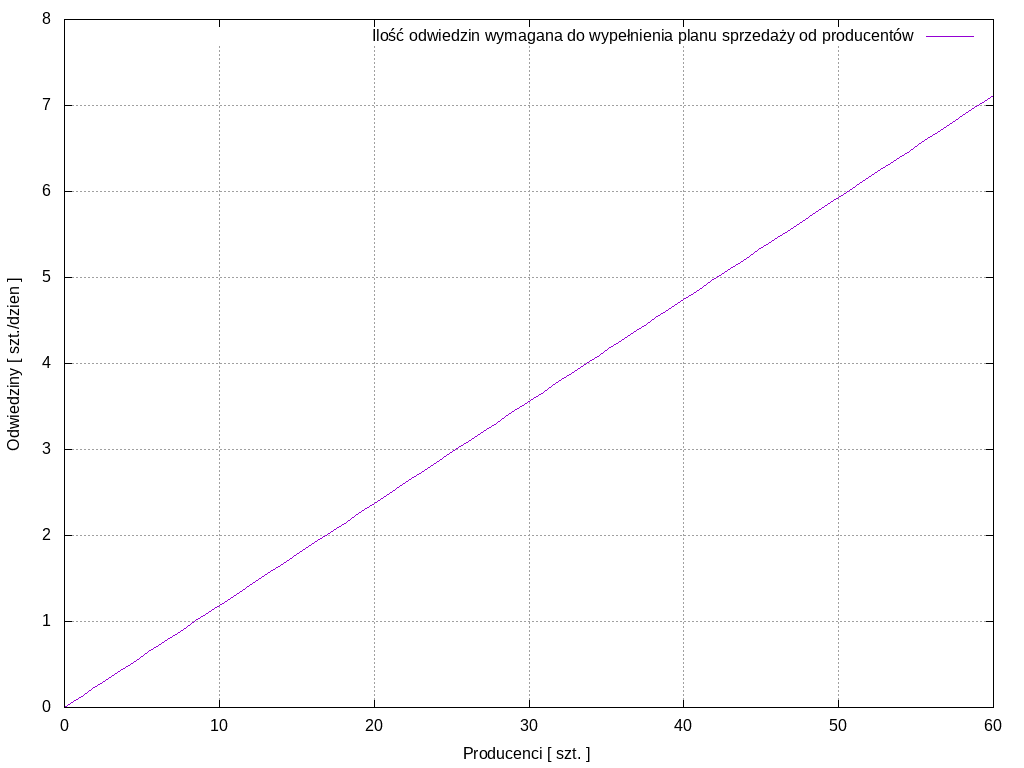
\includegraphics[scale=0.5]{visit_prod}
			\caption{Wykres zależności wymaganych do osiągnięcia średniej sprzedaży odwiedzin strony od producentów}
			\label{visit_prod}
		\end{figure}
		
		Wykresy \ref{income_prod} i \ref{visit_prod} powiązane są ze sobą w następujący sposób do osiągnięcia zakładanej sprzedaży przy danej ilości producentów potrzeba uzyskać przynajmniej taką ilość wejść na stronę od unikalnych potencjalnych klientów jak prezentuje drugi wykres.
		W poprzedniej części ustalono również, że 20\% sprzedaży stanowią meble do sypialni, 5\% stanowią meble kuchenne, a 75\% do salonów i jadalni.
		Ustalając liczbę producentów do pozyskania rocznie na 20 uzyskujemy przewidywany przychód w wysokości 65 tys. zł, który wedle podziału procentowego kategorii przyjmuje następującą postać 13 tys. zł z meble do sypialni, 3.25 tys. z mebli kuchennych, 48.75 tys. mebli do salonów i jadalni.  
		
		Dla kolejnych ustaleń należy jeszcze obliczyć średnią ilość sprzedanych mebli wyraża się ona wzorem:
		
		\[ f(m) = ( s_p + s_k ) \times m = 7.95 \times m \]
		
		\begin{figure}
			\centering
			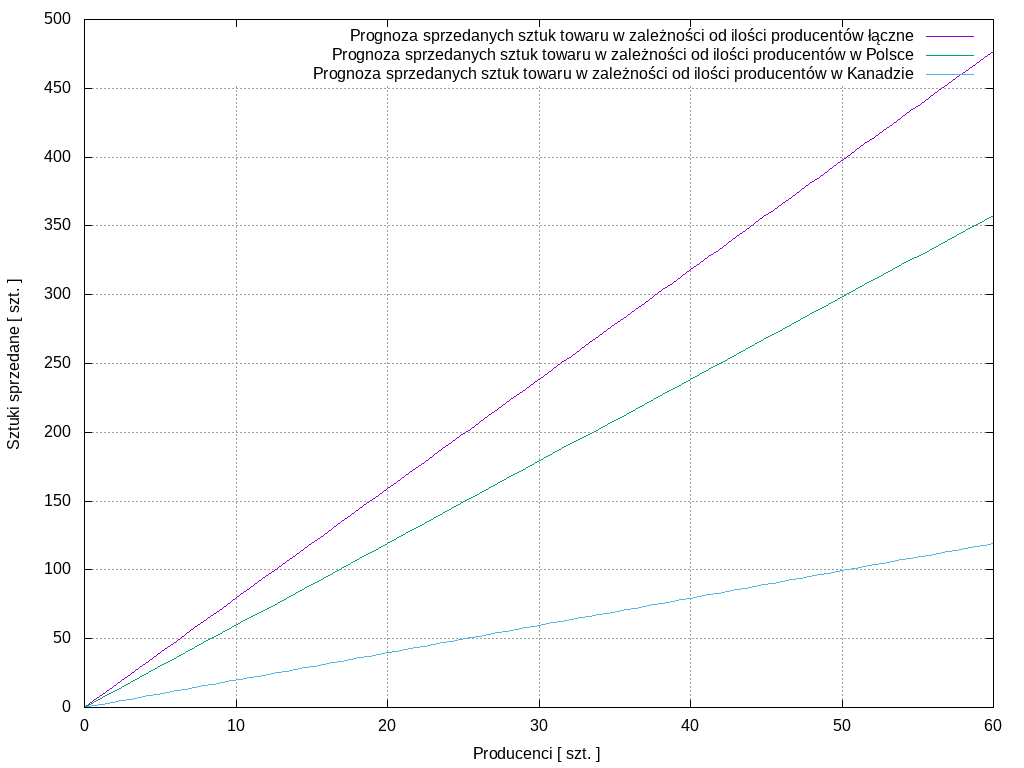
\includegraphics[scale=0.5]{sale_prod}
			\caption{Wykres wymaganej sprzedaży w sztukach od ilości producentów}
			\label{sale_prod}
		\end{figure}

		
	\section{Obecni konkurenci}
		\par W tym przypadku głównymi konkurentami nie są  duże sklepy meblowe, ale mniejsze oferujące niepowtarzalne meble hand-made. Jednym z nich jest sklep "bixbit.com", który posiada meble spersonalizowane o nowoczesnym wzornictwie. "Designconcept.pl" to kolejny sklep "www" oferujący  designerskie meble od różnych producentów. Nie można tu zapomnieć o jednym z największych konkurentów czyli "Meble.pl" działają na rynku od 2008 roku i przez ten czas zdobyli duże zaufanie klientów.
	
	
	\section{Sprzedaż i promocja}
		\par Sprzedaż będzie odbywała się poprzez sklep internetowy na dwóch domenach: sklep-meblowy.org oraz furniture-store.ca. Kluczowym było tu pozyskanie tych domen, ponieważ pozwoli to na zdobycie pozycji rynkowej małym nakładem finansowym. Domeny te to zlepki słów najczęściej wpisywanych według "Google" przez osoby szukające mebli w Polsce jak i w Kanadzie. Wyżej wymienione domeny są już moją własnością. Istotnym elementem sprzedaży i promocji jest wykorzystanie portali takich jak "ebay.ca", "amazon.com" oraz stosunkowo nowo powstały portal "ebid.net", który w samej Kanadzie zdobywa dużą popularność. Na rynku polskim należy skupić się również na portalach "allegro.pl" i "olx.pl"
	
		\par Pod kątem promocji sklepu i pozycjonowania, ważnym elementem jest wykorzystanie stron typu "gumtree.pl", "oglaszamy24.pl" ,"wykop.pl". Tej ostatniej odpowiednikiem o zasięgu globalnym jest "reddit.com".  Nieoceniona będzie również pomoc ze strony płatnych reklam w wyszukiwarce. Nie mówię tu jedynie o wyszukiwarce "google", należy skoncentrować też chociaż część wysiłków na wyszukiwarce wykorzystywanej domyślnie w produktach Microsoftu jaką jest "bing". Oczywiście nie można zapomnieć w tym miejscu o mediach społecznościowych jakimi są "facebook", "twitter" i "instagram", bez których nie da się już prowadzić biznesu. Mój sklep internetowy musi posiadać również  newsletter, który umożliwia rozsyłanie do zarejestrowanych klientów informacji o nowych produktach czy promocjach. W późniejszym etapie prowadzenia firmy, mam zamiar umieszczać reklamy w prasie branżowej np. "M jak mieszkanie", "Weranda" itp., na blogach wnętrzarskich, portalach poświęconych wystrojowi wnętrz. Istnieje też wiele wydarzeń np. targi meblowe, na których warto jest promować swoje produkty.
		
		
	\section{Dostawcy}
		\par Dostawcami w moim sklepie internetowym będą polscy wytwórcy mebli, którzy stawiają duży nacisk na wysoką jakość materiałów, precyzję wykonania i dbałość o najmniejszy szczegół. Zależy mi aby pozyskać małych producentów mebli, którzy swoje siedziby mają na terenie Dolnego Śląska. W trakcie badania rynku zauważyłam, że wiele małych przedsiębiorstw wykonuje niepowtarzalne przedmioty, które znalazłyby wielu nabywców, ale nie mają możliwości sprzedaży ich większej klienteli. 
		\par Dostawców mebli mam zamiar pozyskiwać poprzez przedstawienie im mojej oferty współpracy w sposób bezpośredni, za pośrednictwem portalu takiego jak "biznesoferty.pl", oraz poprzez przesyłanie im ulotki sklepu przygotowanej specjalnie na tą okoliczność.
		
	\section{Technologia i know-how}
		\par Technologią potrzebną dla poprowadzenia tego typu przedsiębiorstwa jest odpowiedni system komputerowy. W jego skład musi wchodzić system obsługi złożenia zamówienia, zarządzania procesem produkcji, oraz system kontroli wysyłki. System obsługi zamówienia musi przekazywać spójne dane dotyczące zamówienia złożonego przez klienta. Tu każdy produkt powinien dostać swój unikalny identyfikator na cały swój cykl życia. System zarządzania produkcją musi zawierać dane o czasie złożenia i zakończenia produkcji, oraz musi umożliwiać przepływ informacji między producentem a centralą firmy. Na samym końcu cyklu realizacji zamówienia system musi powiązać produkt po jego numerze seryjnym i adres klienta umożliwiając łatwe opatrzenie zapakowanego produktu danymi do wysyłki. Dzięki tak przygotowanemu systemowi centrala firmy będzie mieć kontrolę nad zamówieniem od momentu jego złożenia aż do dostarczenia dla klienta. System ten umożliwia też kontrolę jakości, nie tylko pod względem jakości jako takiej, ale również zgodności ze specyfikacją złożoną przez klienta.
		
		\par Dla prowadzenia tego typu działalności potrzebna jest podstawowa wiedza dotycząca prowadzenia firmy, kiedy wystawiać faktury, paragony, a kiedy ich oczekiwać. Przy przedsiębiorstwie eksportowym bardzo istotne jest odpowiednie prowadzenie dokumentacji zdarzeń gospodarczych.

		\par Przydatnym elementem systemów zarządzania jest narzędzie do planowania prac, obrazujące zadania i ich postęp za pomocą wykresu Gantt'a. Wykres pokazuje rozłożenie zadań do wykonania w czasie i osobami przypisanymi do zadań. Poniżej znajduje się przykładowy plan prac:

		\includepdf[pages={1-},scale=0.75]{sklep-meblowy-org-gantt.pdf}

		
		
	

					
	\chapter{Analiza SWOT}
		\section{Analiza SWOT}
	\begin{itemize}	
		\item Mocne strony
			\begin{itemize}
				\item duże doświadczenie w pracy w handlu
				\item wysoka jakość towarów i usług
				\item bardzo dobrze przygotowany system komputerowy
				\item przejrzysty interface sklepu internetowego
				\item niskie koszty prowadzenia działalności
				\item dobra znajomość rynku
				\item sklep międzynarodowy
			\end{itemize}
			
		\item Słabe strony
			\begin{itemize}
				\item niski kapitał własny
				\item brak doświadczenia w prowadzeniu własnej działalności gospodarczej
				\item brak dodatkowych pracowników na początku prowadzenia działalności
				\item brak doświadczenia w handlu międzynarodowym
			\end{itemize}
			
		\item Szanse
			\begin{itemize}
				\item rosnąca zamożność społeczeństwa
				\item łatwa dostępność do sklepu internetowego
				\item rosnące zainteresowanie e-handlem
				\item wprowadzenie kompleksowej umowy gospodarczo-handlowej CETA
			\end{itemize}
			
		\item Zagrożenia
			\begin{itemize}
				\item duża konkurencja
				\item wysokie koszty zakupu sprzętu komputerowego
				\item zaniżanie cen produktów przez konkurencje
				\item niestabilność prawa gospodarczego
				\item brak wystarczającej ilości producentów chętnych współpracować ze sklepem
				\item możliwe rosnące ceny surowców
			\end{itemize}
	\end{itemize}

		
	\chapter{Plan techniczny}
			\section{Wstęp}		
		\par Sprawne działanie przedsiębiorstwa zależy od możliwości przetwarzania informacji, w szczególności w firmach o profilu handlowym. Informacją będzie komunikacja między klientami i przedsiębiorstwem oraz producentami i przedsiębiorstwem. Informacje te możemy podzielić na powstałe w procesach zamówienia, produkcji i dostawy. Przepływem informacji będzie też komunikacja między pracownikami, czy przygotowanie katalogu produktów. Do przepływu informacji możemy również zaliczyć komunikacje z instytucjami administracyjnymi. Celem zapewnienia nieprzerwanego przepływu informacji konieczne jest utworzenie systemu pozwalającego realizować powyższe założenia. Na tej podstawie, przedsiębiorstwo można zobrazować jako centrum wymiany informacji. Wymiana ta zachodzi między grupami pracowników, producentów, klientów i firmami transportowymi.
		
		\begin{figure}[H]
			\centering
			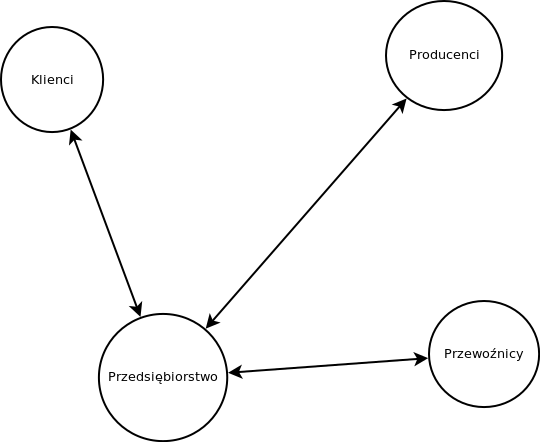
\includegraphics[scale=0.45]{groups}
			\caption{Przepływ informacji między grupami ludzi}
			\label{groups}
		\end{figure} 

	
	\section{Uzasadnienie techniczne}
		\section{System komputerowy}
		\subsection{Koncepcja}
			\par Aby możliwe było zrealizowanie przepływu informacji między grupami ludzi, konieczne jest przygotowanie systemu, który umożliwi komunikację elektroniczną oraz wymianę dokumentów. Komunikacja ta musi odbywać się poprzez system zapewniający bezpieczeństwo informacji, rozumiane jako kontrola dostępu do informacji i zabezpieczenie przed ich utratą. W tym celu należy utworzyć dwa podsystemy, z których jeden będzie odpowiedzialny za zbieranie zamówień i prezentowanie ofert klientom, drugi będzie odpowiadać za prawidłową obsługę procesów w firmie. Pierwszy z systemów nazywany będzie sklepem internetowym, drugi natomiast systemem zarządzania.
	
			\par Funkcjonowanie systemu zarządzania oraz sklepu internetowego wymaga następujących podsystemów pomocniczych: system wiadomości e-mail oraz system baz danych. System wiadomości e-mail odpowiada za przesyłanie korespondencji elektronicznej, natomiast system baz danych za przechowywanie danych pochodzących z poprzednich systemów. 
			%Należy jeszcze sformułować dla tych systemów kroki niezbędne celem zapewnienia bezpieczeństwa i spójności danych.
		
			\par Wymagane elementy można przedstawić za pomocą następującego schematu, w którym strzałki oznaczają przepływ informacji.
		
			\begin{figure}[H]
				\centering
				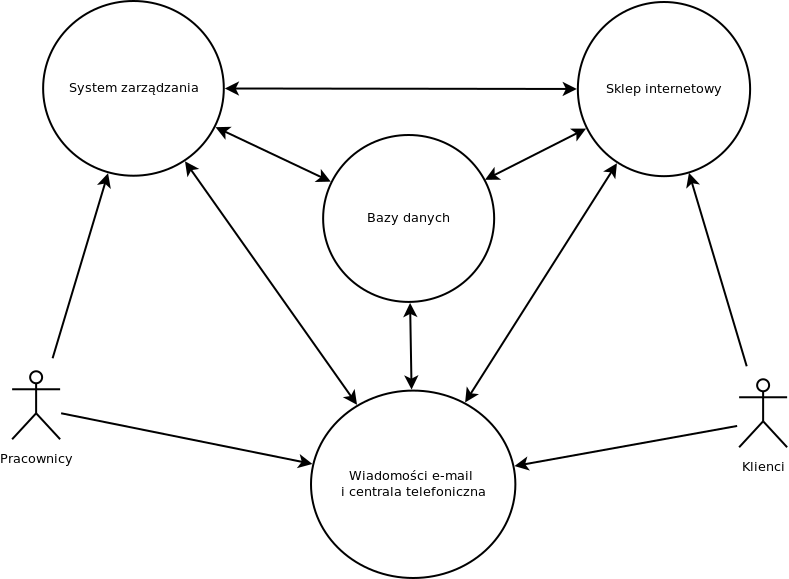
\includegraphics[scale=0.45]{basic_component}
				\caption{Schemat komunikacji poprzez sieć firmową}
				\label{basic_comp}
			\end{figure}
		
			\par Rysunek przedstawia podstawowy diagram przepływu informacji pomiędzy komponentami systemu. Głównym jego elementem jest tu system zarządzania oraz sklep internetowy. System baz danych oraz wiadomości elektronicznych są elementami wymaganymi dla działania dwóch głównych komponentów. Jak pokazuje schemat, dane z systemu zarządzania i sklepu internetowego zapisywane są w bazie danych. Systemy te generują wiadomości e-mail, obsługiwane przez system wiadomości e-mail, który przychodzącą i wychodzącą korespondencje zapisuje w bazie danych. Klienci komunikują się z przedsiębiorstwem poprzez sklep internetowy, wiadomości e-mail oraz rozmowy telefoniczne, natomiast pracownicy przez system zarządzania, wiadomości e-mail i rozmowy telefoniczne.
 
		
		\subsection{Specyfikacja}
			\subsubsection{Wstęp}
				\par Wykorzystując abstrakcyjny schemat komponentów systemu można utworzyć system komputerowy realizujący założoną funkcjonalność. Na podstawie schematu \ref{basic_comp} można przygotować listę programowych komponentów systemu komputerowego. Z powyższego schematu wynika wprost, że system komputerowy musi składać się z: systemu baz danych, systemu plików, centrali telefonicznej, systemu wiadomości e-mail, systemu zarządzania i sklepu internetowego.
				\par Niezbędne jest dodanie do listy składników elementów o znaczeniu technicznym. Będą nimi: system DNS (Domain Resolve System) z ang. system nazw domenowych, odpowiedzialny za tłumaczenie adresów domen na adresy IP. Jest to wymóg rfc1035, aby móc przechowywać domenę, oraz sieciowy system plików, który umożliwi przechowywanie wszystkich danych i współdzielenie ich pomiędzy składnikami systemu.
				
				\par Na podstawie dwóch poprzednich paragrafów można sprecyzować listę składników systemu komputerowego w następujący sposób:
				\begin{itemize}
					\item System DNS
					\item System wiadomości e-mail
					\item Bazy danych
					\item Centrala telefoniczna
					\item Współdzielony system plików
					\item Sklep internetowy
					\item System zarządzania
				\end{itemize}
				
				\begin{figure}[H]
					\centering
					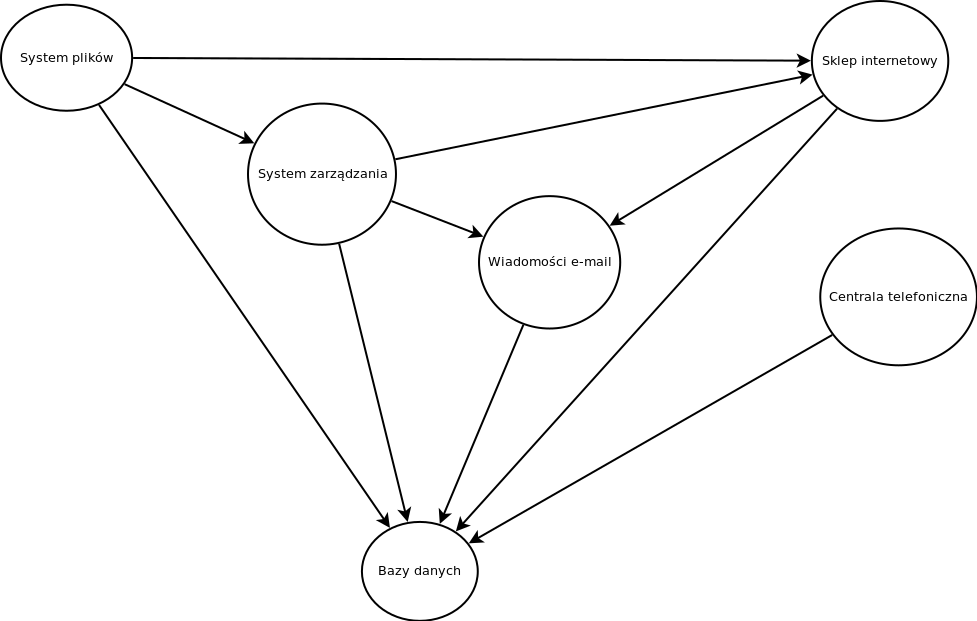
\includegraphics[width=\textwidth]{extended_comp}
					\caption{Schemat składników systemu komputerowego}
					\label{extended_comp}
				\end{figure}
			
			\subsubsection{Opis}
				\par Wymienione uprzednio składniki systemu komputerowego, którymi są: system DNS, system wiadomości e-mail, bazy danych, centrala telefoniczna, współdzielony system plików, sklep internetowy oraz system zarządzania umożliwiają komunikację między między pracownikami i klientami sklepu. Dzięki następującym funkcjonalnością:
				
				\begin{description}
						\item[System DNS] - system odpowiedzialny za przechowywanie domen sklepu internetowego, jego zadaniem jest kierowanie klientów do odpowiednich serwerów poprzez tłumaczenie zrozumiałych dla człowieka nazw na adresy występujące w sieciach komputerowych. Przykładem może być nazwa domenowa \textit{sklep-meblowy.org}, której adres sieciowy to \textit{188.122.10.34}.
						
						\item[Wiadomości e-mail] - system ten odpowiada za odbieranie i wysyłanie poczty elektronicznej.
						
						\item[Bazy danych] - system ten odpowiada za przechowywanie danych ze sklepu internetowego, oraz systemu zarządzania. Składowane są na nim również dane danych z systemu wiadomości e-mail, oraz centrali telefonicznej. 
				
						\item[Centrala telefoniczna] - system ten umożliwia użytkowanie usługi telefonii VOIP ( z ang. Voice Over IP - głos poprzez IP ). Służy ona przekazywaniu rozmów telefonicznych poprzez internet. Dzięki temu można wykonywać połączenia międzynarodowe bez konieczności ponoszenia kosztów międzystrefowych. Realizuje ona również funkcję nagrywania połączeń przychodzących i wychodzących.  
				
						\item[Współdzielony system plików] - system ten odpowiada za przechowywanie danych pochodzących od pozostałych składników. Na nim zapisywane będą bazy danych, wiadomości e-mail, rozmowy telefoniczne itp. Jego najważniejszą cechą jest możliwość współdzielenia danych oraz miejsca do ich zapisu.
				
						\item[Sklep internetowy] - składnik ten umożliwia klientom dostęp do produktów sklepu, tworzenie kont indywidualnych i biznesowych, oraz najważniejsze- możliwość zakupu wybranego towaru.
					
						\item[System zarządzania] - składnik ten umożliwia organizację pracy pod kątem planowania produkcji i logistyki towaru. W jego skład wchodzą: moduły umożliwiające wystawianie faktur, prowadzenie historii operacji finansowych czy tworzenie grafików pracy. 
					\end{description}
 
				
		\subsection{Implementacja}
			\subsubsection{Wstęp}
				\par Implementacje systemu komputerowego należy podzielić na środki programowe i sprzętowe. Do środków programowych zaliczamy oprogramowanie realizujące funkcjonalność opisanych w wcześniej składników systemu. Środkami sprzętowymi będą komputery oraz osprzęt sieciowy niezbędny do utworzenia sieci komputerowej.
				
			\subsubsection{Środki programowe}
				\par Korzystając z poprzednich informacji można ustalić podstawowy schemat komponentów programowych. System zarządzania oraz sklep internetowy muszą znajdować się na serwerze www. Oprogramowanie to jest odpowiedzialne za wygenerowanie dynamicznej strony internetowej na żądanie klienta lub pracownika sklepu. Następnym elementem będzie serwer wiadomości e-mail odpowiedzialny za komunikację elektroniczną. Kolejnym elementem systemu jest serwer centrali telefonicznej odpowiedzialny za połączenia przychodzące i wychodzące. Elementem wymaganym przez poprzednie składowe systemu jest serwer baz danych, na którym zapisywane będą dane pochodzące z poprzednich serwerów. Przedostatnim elementem jest serwer sieciowego systemu plików, na którym zapisywane będą dane pochodzące z serwera baz danych oraz wszystkie pozostałe pliki. Ostatnim elementem będą dwa serwery DNS, które są wymagane do samodzielnego przechowywania domeny.
				
				Lista serwerów potrzebnych do zrealizowania założeń obsługi klienta i funkcjonowania firmy: 
				\begin{itemize}
					\item Dwa serwery DNS
					\item Serwer wiadomości e-mail
					\item Serwer baz danych
					\item Centrala telefoniczna
					\item Serwer sieciowego systemu plików
					\item Serwer www
				\end{itemize}
			
				\par Na podstawie powyższej listy można przygotować podstawowy schemat systemu komputerowego. Należy rozszerzyć go o wcześniej nie wspomniane elementy jakimi są router i most sieciowy. Router'em nazywamy urządzenie komputerowe odpowiadające za trasowanie informacji na poziomie programowym do odpowiednich elementów systemu. Natomiast most sieciowy jest elementem spajającym wszystkie elementy sieci w spójną całość.
			
				\begin{figure}[H]
					\centering
					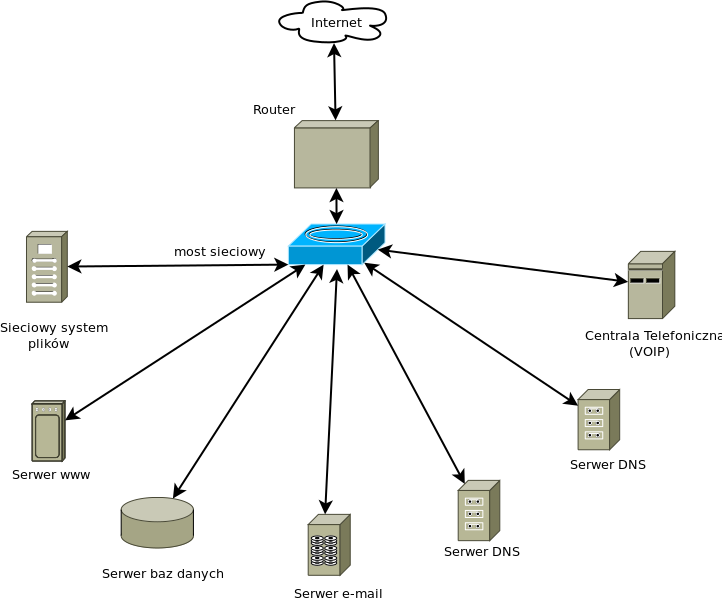
\includegraphics[scale=0.45]{Basic}
					\caption{Podstawowy schemat sieci}
					\label{basic_net}
				\end{figure}
				
				\par Serwery przedstawione na schemacie \ref{basic_net} mogą być komputerami fizycznymi lub komputerami wirtualnymi. Technologia wirtualizacji w systemach serwerowych pozwala utworzyć na komputerze fizycznym komputery wirtualne korzystające z jego zasobów. Innymi słowy na jednym fizycznym komputerze można uruchomić kilka komputerów wirtualnych. 
		
				\paragraph{Serwer wirtualny}
				\par Jako serwer wirtualny definiujemy proces umożliwiający uruchomienie komputera wirtualnie wraz z systemem operacyjnym pod kontrolą innego działającego już systemu operacyjnego. Serwer tego typu nazywany będzie serwerem VPS od angielskiego Virtual Private Server czyli wirtualnego serwera prywatnego.
		
			\subsubsection{Środki sprzętowe}	
				\par Do środków sprzętowych zaliczone zostaną komputery, router lub access point (AP), kasa fiskalna, oraz drukarka sieciowa. Poniższa lista w krótki sposób charakteryzuje wymienione sprzęty.
				
				\begin{description}
					\item[Serwery] - stanowią fundament firmy gdyż na nich znajdować się będzie sklep, centrala telefonii VOIP, serwis mailowy, infrastruktura sieci i bazy danych. Właśnie stąd sklep będzie hostowany na cały świat i to z serwerami będą łączyć się klienci.

					\item[Kasa fiskalna] - służy księgowaniu transakcji. Potrzebna będzie kasa walutowa pobierająca aktualne kursy walut, gdyż część transakcji będzie obejmowała klientów zagranicznych.

					\item[Przełącznik PoE] - urządzenie pozwalające na przyłączenie wielu urządzeń sieciowych do sieci komputerowej. Pozwoli to skonsolidować wszystkie elementy składowe sieci.

					\item[Macierz dyskowa] - komputer zawierający kilka dysków fizycznych przechowujących dane całej sieci. Dyski te połączone są w grupę "RAID", co gwarantuje bezpieczne przechowywanie dużych ilości danych. Takie rozwiązanie ma wymieniać dane pomiędzy serwerami, co zwiększa integralność sieci.

					\item[Drukarka sieciowa ze skanerem] - podstawowe wyposażenie biurowe; zestaw ten jest konieczny do drukowania, kserowania jak i skanowania dokumentów. 

					\item[Telefon voip] - telefon zostanie zastąpiony telefonią VOIP ze względu na wysokie stawki połączeń międzynarodowych przy standardowym połączeniu telefonicznym. Dzięki telefonii internetowej ze względu na używanie transferu opłaconego w abonamencie za usługi internetowe, będziemy mogli bez dodatkowych kosztów obsługiwać połączenia wychodzące jak i przychodzące.

					\item[Access Point] - pozwala na dostęp do sieci komputerowej za pomocą WiFi. Urządzenie to wykorzystywane będzie przez pracowników do podłączenia się do internetu jak i sieci lokalnej.
				\end{description}
				
				\par Jako serwer lub macierz dyskową należy rozumieć komputer świadczący w sieci komputerowej określone usługi na rzecz serwerów lub ludzi. Jako komputer należy rozumieć zespół połączonych ze sobą komponentów elektronicznych i elektromechanicznych jakimi są:
				
				\begin{description}
						\item{Procesor} - Elektroniczne urządzenie cyfrowe odpowiadające za pobieranie i przetwarzanie instrukcji. 
			
						\item{Płyta główna} - Element elektroniczny, na którym zamontowane są pozostałe podzespoły komputera. Umożliwia ona komunikację pomiędzy pozostałymi komponentami komputera.
			
						\item{Pamięć operacyjna} - Urządzenie elektroniczne umożliwiające przechowywanie wykonywanych programów, ich danych oraz wyników działania.
			
						\item[Dysk twardy] - Urządzenie elektroniczno-mechaniczne umożliwiające trwałe zapisanie wprowadzonych danych.
			
						\item[Karta sieciowa] - Komponent elektroniczny umożliwiający podłączenie komputera do sieci wraz z innymi komputerami i urządzeniami.
			
						\item[Karta graficzna] - Element elektroniczny umożliwiający wyświetlenie obrazu z komputera na odpowiednim wyświetlaczu.
			
						\item[Zasilacz] - Urządzenie elektromechaniczne dostarczające zasilanie do pozostałych podzespołów systemu komputerowego.
			
						\item[Obudowa] - Umożliwia umieszczenie i zamocowanie najważniejszych elementów komputera.
				\end{description}
				
				\subsubsection{Specyfikacja sieci}
					\par Wykorzystując wcześniej opracowane dane można przygotować specyfikację sieci prezentowaną przez schemat \ref{office}. Przedstawia ona środki sprzętowe niezbędne do zrealizowania wyznaczonych zadań.
			
					\begin{figure}[H]
						\centering
						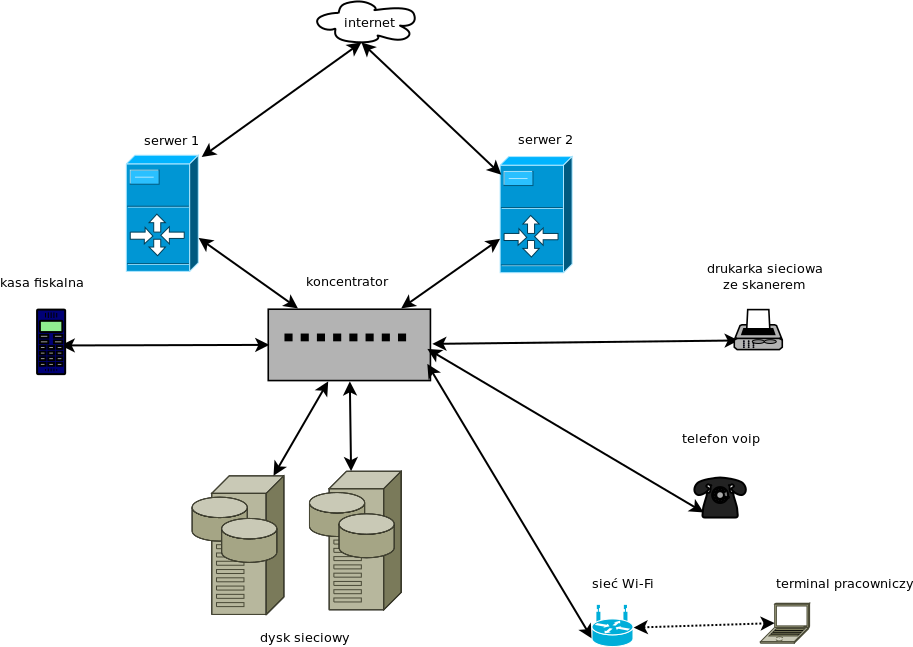
\includegraphics[scale=0.45]{Diagram1}
						\caption{Specyfikacja sieci biurowej}
						\label{office}
					\end{figure}
				
					\par Poniższy diagram przedstawia środki programowe niezbędne do realizacji założonych zadań umieszczone na dwóch serwerach, oraz współdzielony system plików na macierzy dyskowej. 
		
					\begin{figure}[H]
						\centering
						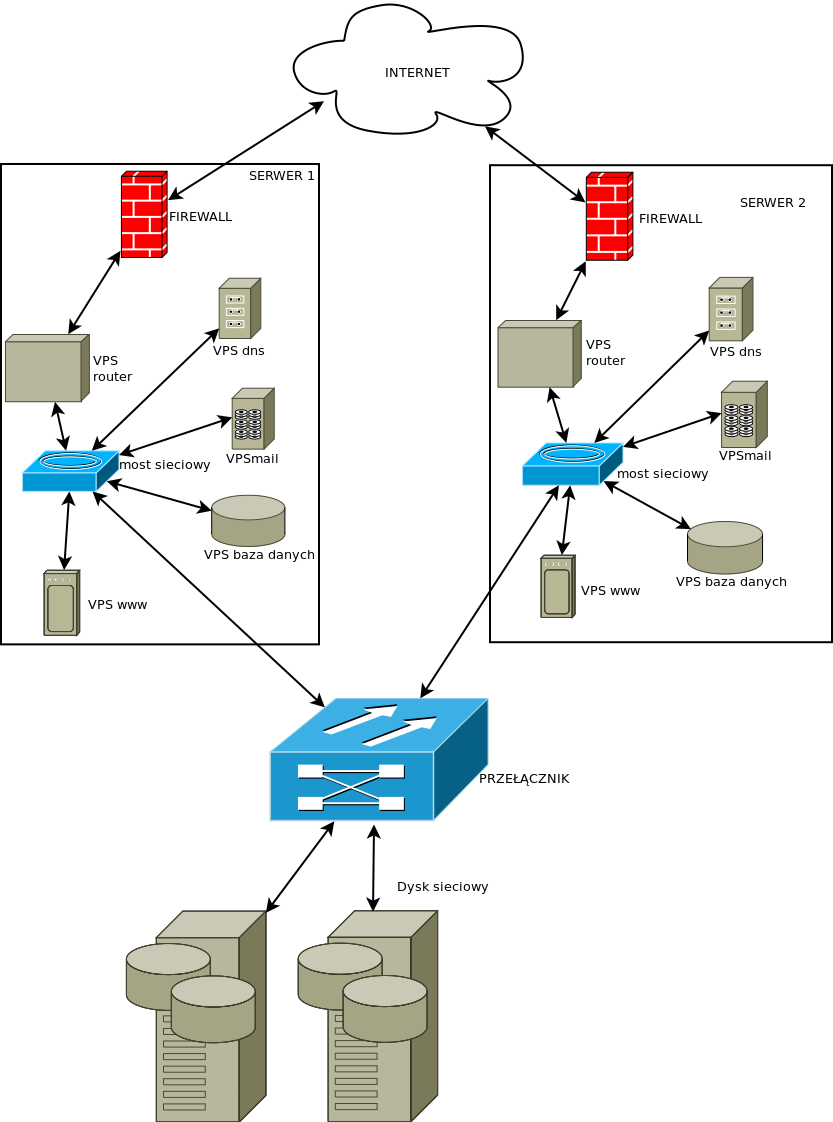
\includegraphics[scale=0.45]{Diagram2}
						\caption{Diagram środków programowych na serwerach}
						\label{net_real}
					\end{figure}
				
					\par Wykorzystana architektura systemu komputerowego nosi nazwę "failover cluster" wraz z technologią "load balancing". Jest to układ komputerów i oprogramowania, którego celem jest równoważenie obciążenia realizowanych zadań między zdublowane komponenty wykonujące te same funkcje. Oprócz tego umożliwia działanie systemu w przypadku awarii Serwera 1, lub Serwera 2, ze zmniejszoną wydajnością.
 
				
		\subsection{Opis systemu zarządzania}	
			\par System zarządzania jest narzędziem umożliwiającym planowanie, organizowanie i kontrolowanie postępów w pracy nad wieloma projektami i zadaniami. Każdy użytkownik może mieć różne uprawnienia przy różnych projektach, a manager i administrator mają pełną kontrolę nad swoimi zasobami.
			\par Utworzenie tego narzędzia w formie aplikacji internetowej, obsługiwanej przez dedykowany serwer umożliwia użytkownikom swobodny dostęp do informacji z dowolnego miejsca, o dowolnym czasie. Analogicznie osoby do tego uprawnione, w każdym momencie mogą zarządzać projektami i wprowadzać zmiany.
			\par System daje możliwość organizacji nieskończonej ilości niezależnych projektów. Przy każdym projekcie możemy zdefiniować typy zagadnień jak i moduły: Śledzenie zagadnień, Śledzenie czasu, Komunikaty, Dokumenty, Pliki, Wiki, Fora, Repozytorium, Diagram Gantta, Kalendarz oraz wiele innych.
			\par Systemy zarządzania dzielimy na dwie kategorie. Pierwszą kategorią są systemy zarządzania relacji z klientami nazywane z ang. CRM (Client Relation Managment), drugą systemy zarządzania zasobami przedsiębiorstwa nazywane z ang. ERP (Enterprise Resource Planning).
			\par Wybrany system zarządzania to "redmine" wraz z modułami CRM i Commerce. Jest to aplikacja internetowa napisana w języku ruby. Współpracuje ona z bazą danych PostgreSQL i jest często wykorzystywana do zarządzania projektami różnego typu. W tym wypadku możemy potraktować każdą sprzedaż jako osobny projekt składający się z kilku procesów.

			\input{oferta_organizacja_system_zarzadzania_skladniki.tex}
 
				
		\subsection{Sklep internetowy}	
			\input{oferta_organizacja_sklep_internetowy.tex} 

		\subsection{Charakterystyka systemu}
			\par Zaproponowany system komputerowy charakteryzuje się następującymi cechami:
				
				\begin{itemize}
					\item Bezpieczeństwem przechowywania danych
					\item Niezawodnością
					\item Wydajnością
					\item Pojemnością
				\end{itemize}
		
				\subsubsection{Bezpieczeństwo przechowywania danych}
					Aby zadbać o bezpieczeństwo danych należy przedsięwziąć odpowiednie kroki zmierzające do ich ochrony:
				
					\begin{description}
					
						\item[\textbf{Redundancja danych}] Zabezpieczenie polegające na przechowywaniu danych w dwóch kopiach. Wszystkie istotne dane pojawiające się w systemie przechowujemy wraz z kopią zapasową. Co najistotniejsze, kopia ta tworzona jest w czasie rzeczywistym. Dzięki temu potrzebne dane chronione są od momentu powstania.
				
						\item[\textbf{Utrzymanie wersji produkcyjnej i rozwojowej}] Strategia ta zakłada utrzymanie wersji rozwojowej i produkcyjnej oprogramowania, zarówno w zakresie sklepu internetowego jak i systemu zarządzania. Wszystkie zmiany w funkcjonowaniu sklepu muszą zostać wprowadzone najpierw na wersji rozwojowej, gdzie zostaną gruntownie przetestowane, a dopiero po zatwierdzeniu wprowadzane do wersji produkcyjnej. 
						
						\item[\textbf{Zabezpieczenie baz danych}] Dla bazy danych sklepu internetowego i systemu zarządzania należy skonfigurować PITR (Point In Time Recovery), powrót do punktu w czasie. Jest to rozwiązanie wykorzystywane np. przy systemach przeprowadzających operacje finansowe. W razie awarii możliwe jest odtworzenie stanu systemu z dokładnej daty sprzed awarii. Mechanizm ten zapisuje historię operacji wykonywanych na bazie danych wraz z dokładną datą. Dzięki temu bazę danych zabezpieczoną tym mechanizmem można odtwarzać operacja po operacji.

					\end{description}
					
			\subsubsection{Niezawodność}
					\par Celem analizy niezawodności systemu komputerowego należy zaznajomić się ze statystykami awaryjności sprzętu elektronicznego. Pierwszy wykres przedstawia statystyki awaryjności sprzętu produkowanego przez danego producenta. Wykres ten pozwala ustalić średnią awaryjność w ciągu pierwszego, drugiego i trzeciego roku użytkowania sprzętu, oraz trzyletniego czasu użytkowania. 
				
					\begin{figure}[H]
						\centering
						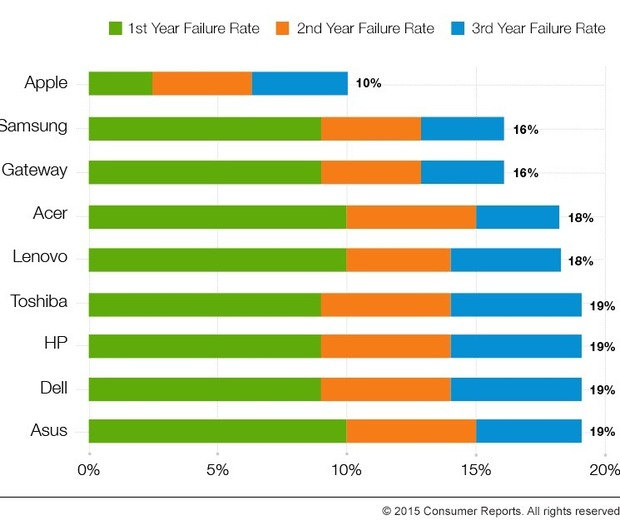
\includegraphics[scale=0.35]{consumer_reports_failures}
						\caption{Raport awaryjności sprzętu elektronicznego}
						\label{rep_fail}
					\end{figure}
				
				\par Na podstawie wykresu \ref{rep_fail} można określić, że prawdopodobieństwo awarii w pierwszym roku wynosi ok. 8 \%, a w roku drugim i trzecim ok. 5\%. Na tej podstawie można stwierdzić, że 20\% zakupionego sprzętu elektronicznego zepsuje się w przeciągu 3 lat użytkowania. Należy zapoznać się również z tzw. "krzywą wanny" prezentującą awaryjność sprzętu elektronicznego. Można odczytać z niej bardzo istotne informację. Pierwszy obszar wykresu obejmuje początek cyklu życia produktu. Prawdopodobieństwo awarii produktu w tym obszarze jest największe na początku cyklu i spada po krzywej hiperbolicznej aż do ustabilizowania się w etapie drugim. Na pierwszym etapie duża awaryjność jest powodowana błędami w produkcji, prześliźnięciem się produktu przez kontrolę jakości itp. Na drugim etapie mamy stały odsetek awarii sprzętowych. Wynika to ze zwykłej losowości i praw Murphy'iego - rzeczy się psują. Na końcowym etapie życia produktu krzywa awarii znów przybiera postać hiperboli i dość szybko zmierza ku górze. Na tym etapie podatność na awarię wzrasta i wynika ona z takich czynników jak: zużycie, zmęczenie materiałów itp. Należy pamiętać, że elementy użyte w sprzęcie mają określoną ilość godzin pracy, cykli odczytu/zapisu itp. lub zostały zaprojektowane z takich materiałów, aby popsuły się po okresie gwarancyjnym. 
				
				\begin{figure}[H]
					\centering
					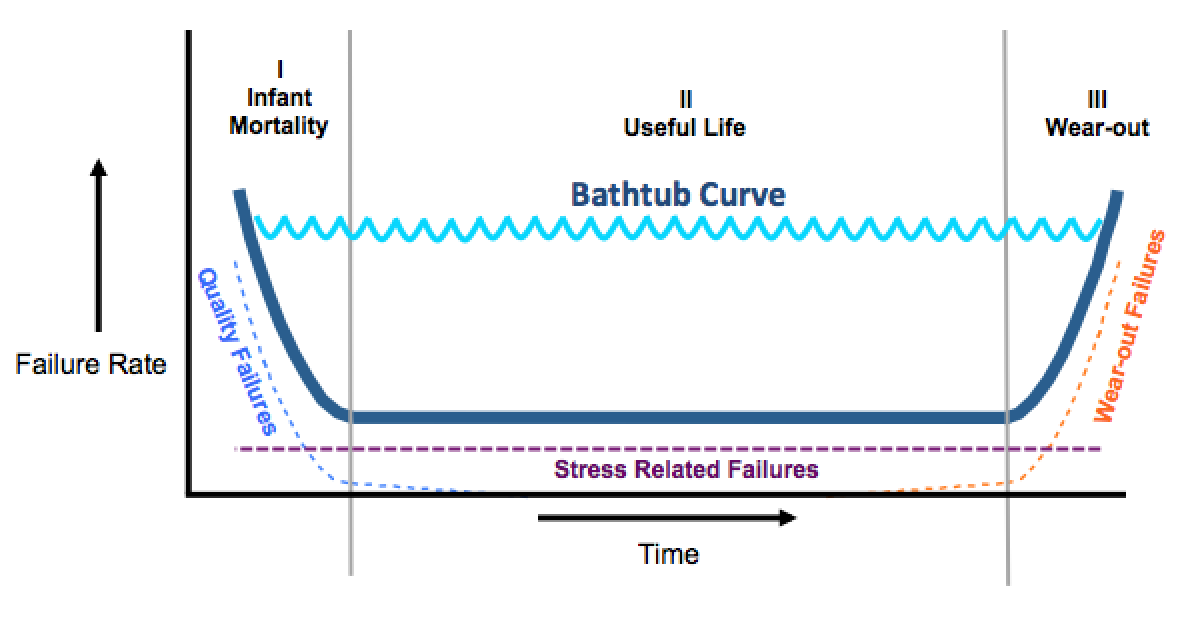
\includegraphics[scale=0.35]{bath_curve}
					\caption{Krzywa wanny prezentująca awaryjność sprzętu}
				\end{figure}

				\par Niezawodności należy rozpatrywać pod katem dwóch przypadków. Pierwszym z nich jest niezawodność programowa, drugą zaś niezawodność sprzętowa platformy. W jednym i drugim przypadku, rozwiązaniem jest duplikacja elementów systemu wykonujących te same zadania. Koncepcję tą z powodzeniem można wytłumaczyć odwołując się do rozkładu dwumianowego, nazywanego też schematem Bernoulli'ego.
				
				\[ P_n(k) = \binom{n}{k} p^k (1-p)^{n-k} \]
			
				gdzie:
			
				\begin{description}
					\item n - ilość prób 
					\item k - ilość sukcesów 
					\item p - prawdopodobieństwo sukcesu
				\end{description}
				
				Wzór ten opisuje nam prawdopodobieństwo uzyskania "k" sukcesów w "n" próbach. Przyjmując jako "sukces" wystąpienie awarii można policzyć niezawodność systemu. 
			
				\begin{enumerate}
					\item W przypadku jednego urządzenia wykonującego dane zadanie należy wziąć pod uwagę uśrednione dane z histogramu:
							\begin{itemize}
								\item Prawdopodobieństwo awarii w pierwszym roku wynosi 8\%, w drugim i trzecim 5\%
								\item Prawdopodobieństwo awarii przez cykl 3 lat wynosi 18%
							\end{itemize}
					\item w przypadku dwóch urządzeń realizujących tą samą funkcję, zakładając że wystarczy jeden z nich otrzymujemy:
							\begin{itemize}
								\item Prawdopodobieństwo awarii w pierwszym roku \( P_2(2) = \binom{2}{2} 0.08^2 (1-0.08)^{2-2} = 0.0064*100\% = 0.64\%\)
								\item Prawdopodobieństwo awarii w drugim i trzecim roku \( P_2(2) = \binom{2}{2} 0.05^2 (1-0.05)^{2-2} = 0.0025*100\% = 0.25\%\)
								\item Prawdopodobieństwo awarii przez cykl 3 lat wynosi \( P_2(2) = \binom{2}{2} 0.18^2 (1-0.18)^{2-2} = 0.0324*100\% = 3.24\%\)
								\item Prawdopodobieństwo awarii jednego z dwóch urządzeń przez cykl 3 lat wynosi \( P_2(1) = \binom{1}{2} 0.18^1 (1-0.18)^{2-1} = 0.2952*100\% = 29.52\%\)
							\end{itemize}
				\end{enumerate}
				
				\par Jak wynika z przeprowadzanych rozważań, celem ochrony danych oraz logicznej separacji systemu komputerowego, należy rozdzielić elementy przetwarzające oraz przechowujące dane. Celem osiągnięcia pożądanej jak najniższej awaryjności, należy podzielić system komputerowy na dwie grupy. Pierwszą z nich będzie grupa przetwarzająca dane a druga będzie grupą przechowującą dane. Z przeprowadzonych obliczeń wynika, że prawdopodobieństwo awarii krytycznej w każdej grupie wynosi 3.24\%. Na tej podstawie, dla 3 letniego cyklu użytkowania sprzętu, można wysnuć następujące wnioski:
				
				\begin{itemize}
					\item Prawdopodobieństwo awarii krytycznej tzn. uniemożliwiającej dalszą pracę systemu wynosi 3.24\% w czasie 3 lat
					%\item Prawdopodobieństwo awarii krytycznej całego systemu wynosi 0.1\% 
					\item Prawdopodobieństwo awarii nie krytycznej tzn. wpływającej jedynie na wydajność systemu wynosi 8.71\% w okresie roku i 29.52\% w okresie 3 lat
				\end{itemize}
			
			\subsubsection{Wydajność}
				\par Celem zapewnienia optymalnego przetwarzania żądań system komputerowy musi charakteryzować się wydajnością rozumianą jako zestaw parametrów określających jego możliwości. Tymi parametrami są ilość rdzeni procesora oraz rozmiar pamięci operacyjnej. Poniższa lista prezentuje minimalne parametry jakie muszą posiadać serwery, aby przetwarzanie danych było możliwe. 
				
				\begin{itemize}	
						\item{\textbf{serwer DNS}} Wystarczające będzie zarezerwowanie 1 rdzenia procesora i 2GB pamięci operacyjnej, ze względu na wykonywania nieskomplikowanych zadań jakimi jest tłumaczenie nazw mnemonicznych na adresy sieciowe.
						
						\item{\textbf{serwer E-Mail}} Ze względu na filtrowanie wirusowe i filtrowanie spamu, czyli niechcianej poczty. Należy na niego zarezerwować 2 rdzenie procesora oraz 4GB pamięci operacyjnej.
						
						\item{\textbf{serwer Baz danych}} Wydajność pozostałych systemów zależy od szybkości realizacji zapytań na bazach danych, serwer ten musi być wydajny. Ze względu na to zarezerwowane dla niego zostaną 4 rdzenie procesora, oraz 4 GB pamięci operacyjnej.
						
						\item{\textbf{centrala telefoniczna}} Ze względu na nagrywanie rozmów, bezpieczne będzie przydzielenie tu 3 rdzeni procesora oraz 4 GB pamięci operacyjnej. 
						
						\item{\textbf{współdzielony system plików}} Musi posiadać on co najmniej 2 rdzenie procesora i 8 GB pamięci operacyjnej na pamięć pośrednią otwartych plików, oraz ze względu na to, że jego wydajność jest kluczowa dla działania wszystkich innych podsystemów.
						
						\item{\textbf{serwer www}}  Ze względu na konieczność generowania dynamicznej strony internetowej przygotowanej w języku skryptowym, oraz świadczenie jej klientom za pomocą serwera http. Wymagać to będzie co najmniej 2 rdzeni procesora i co najmniej 4GB pamięci operacyjnej.
					
					\end{itemize}	
			
					Po przeprowadzeniu wstępnej analizy wydajnościowej udało się ustalić, że dla budowy minimalnego systemu potrzeba komputera posiadającego:
			
					\begin{itemize}
						\item 15 rdzeni procesora
						\item 28GB pamięci operacyjnej
					\end{itemize}
			
					\par Ważnym parametrem procesora jest również pamięć podręczna, nazywana z angielskiego pamięcią "cache". Odpowiada ona za magazynowanie instrukcji wykonywanych przez procesor. Instrukcje te są magazynowane w czasie gdy procesor przetwarza instrukcje wcześniej zmagazynowane. Odpowiedni dobór wielkości pamięci podręcznej pozwala na optymalne wykorzystanie technologii przetwarzania wielowątkowego. Dzięki wykorzystaniu przetwarzania wielowątkowego jeden rdzeń procesora może pracować jako dwa. Pozwoli to ograniczyć ilość rdzeni procesora dwukrotnie, z 15 do 8, jednak pociąga za sobą konieczność posiadania przez procesor co najmniej 2MB pamięci podręcznej na rdzeń fizyczny. Pozwala to określić specyfikacje komputera:
			
					\begin{itemize}
						\item 8 rdzeni fizycznych procesora
						\item 28GB pamięci operacyjnej
						\item obsługa technologii HyperThreading (przetwarzania wielowątkowego)
						\item 16MB pamięci podręcznej
					\end{itemize}
					
			\subsubsection{Pojemność}
				\par Ilość danych zależeć będzie też od funkcjonowania systemu. Głównym źródłem danych będą tu procesy związane z obsługą klienta. Poniższa lista prezentuje dane, jakie należy zabezpieczyć celem bezpiecznej realizacji procesów zamówienia i reklamacji.
	
					\begin{itemize}
						\item Zamówienie klienta
							\begin{itemize}
								\item Dane dotyczące zamówienia, pozwalające jednoznacznie określić wszystkie wymagania klienta co do tworzonego produktu.
								\item Zlecenie produkcji przesyłane do producenta będące specyfikacją wedle której wykonany ma zostać dany produkt.
								\item Dokumenty powstałe w procesie zamówienia tj. faktury, paragony, dokumenty transportowe, kopie paragonów.
							\end{itemize}
						\item Reklamacja klienta
							\begin{itemize}
								\item Zdjęcia uszkodzonego produktu i zgłoszenie reklamacji.
								\item Dokumenty powstałe w procesie reklamacji tj. faktury, dokumenty transportowe, decyzja.
							\end{itemize}
						\item Rozmowy telefoniczne
							\begin{itemize}
								\item Rozmowy telefoniczne z klientami.
								\item Rozmowy telefoniczne z producentami.
							\end{itemize}
					\end{itemize}
		
					\par Dla obliczenia ilości, należy ustalić parametry, związane z wymienionymi wcześniej czynnościami i procesami. Określenie ich niezbędne jest do oszacowania ilości danych zbieranych podczas obsługi klientów i funkcjonowania sklepu. 
		
					\begin{itemize}
						\item Zmienne globalne 
							\begin{description}
								\item \( R_z \) średni rozmiar zdjęcia
								\item \( Z_r \) przewidywana ilość zamówień rocznie
								\item \( L_p \) wymagane lata przechowywania danych
								\item \( H_m \) średni rozmiar wiadomości e-mail
								\item \( C_r \) średni rozmiar minuty rozmowy
								\item \( D_s \) średni rozmiar jednego dokumentu
								\item \( R_r \) współczynnik reklamacji
							\end{description}
						\item Zmienne określające parametry potrzebne do wyliczenia ilości danych potrzebnych na informacje o produktach od producentów
							\begin{description}
								\item \( M_p \) średnia ilość mebli od producenta
								\item \( Z_p \) średnia ilość zdjęć na produkt
								\item \( P_w \) ilość współpracujących producentów
							\end{description}
						\item Zmienne określające parametry potrzebne do wyliczenia ilości danych potrzebnych na prawidłowe zabezpieczenie procesu zamówienia
							\begin{description}
								\item \( O_z \) średnia ilość zdjęć na zamówienie 
								\item \( L_z \) średnia ilość zdjęć z produkcji 
							\end{description}
						\item Zmienne określające parametry potrzebne do wyliczenia ilości danych potrzebnych do utrwalenia komunikacji
							\begin{description}
								\item \( X_r \) średni czas rozmowy telefonicznej w minutach
								\item \( M_c \) średnia ilość pozostałych wiadomości e-mail dziennie
								\item \( K_l \) średnia ilość telefonów na zamówienie
								\item \( T_p \) średnia ilość wiadomości e-mail na zamówienie
							\end{description}
						\item Zmienne określające ilość zużytych danych od przechowywanych dokumentów
							\begin{description}
								\item \( D_z \) średnia ilość dokumentów powstałych w procesie zamówienia
							\end{description}
						\end{itemize}
		
						\par Kolejnym krokiem jest wyznaczenie funkcji opisujących ilość powstałych danych od czynności wykonanych w procesach i czynników takich jak ilość producentów i zamówień.
		
						\begin{itemize}
							\item Zależność przedstawiająca ilość zużycia danych od ilości produktów i producentów. 
								\[  Z_{mp} = R_z \times M_p \times Z_p \times P_w \]
					
							\item Zależność przedstawiająca ilość zużycia danych od ilości zamówień
								\[ Z_{mz} = ( O_z + L_z) \times R_z \times Z_r \times L_p \]
								
							\item Zależność przedstawiająca zużycie miejsca od ilości telefonów i mail'i
								\[ Z_{km} = (Z_r \times X_r \times K_l + M_c \times H_m \times 365 + T_p \times M_c \times Z_r ) \times L_p \]
								
							\item Zależność przedstawiająca ilość zużytych danych od przechowywanych dokumentów
								\[ Z_{dm} = D_z \times D_s \times Z_r \times L_p \]
						\end{itemize}
		
						Na podstawie powyższych funkcji możemy przedstawić ilość miejsca zajętego przez dane jako sumę wcześniej ustalonych funkcji.
		
						\[ Z_a = Z_{mp} + Z_{mz} + Z_{km} + Z_{dm} \]

						Do powstałego wzoru należy doliczyć jeszcze współczynnik reklamacji. W procesie reklamacji prawdopodobnie powstanie tyle samo danych co w procesie zamówienia. Jednak procesów reklamacji będzie odpowiednio mniej niż zamówień. Aby obliczyć ilość powstałych danych, należy powiększyć dane pochodzące z obsługi sprzedaży o dane powstałe w procesie reklamacji. Przyjmując współczynnik reklamacji wyrażony w procentach można przyjąć, że ilość danych z każdej funkcji należy pomnożyć przez \( 1 + R_r \).
			
						\[ Z_a = Z_{mp} + (1 + R_r) \times Z_{mz} + (1 + R_r) \times (1 + R_r) \times Z_{km} + (1 + R_r) \times Z_{dm} \]
			
						Pamiętajmy o zastosowaniu technologii redundancją danych na wypadek awarii, dzięki czemu wszystko przechowujemy w dwóch kopiach 
						
						\[ Z_a = 2 \times ( Z_{mp} + (1 + R_r) \times Z_{mz} + (1 + R_r) \times Z_{km} + (1 + R_r) \times Z_{dm} ) \]
						
						Ustalmy teraz wartości zmiennych potrzebne do obliczenia ilości potrzebnego miejsca
		
						\begin{itemize}
							\item \( R_z = 1MB \)
							\item \( L_p = 5 lat \) 
							\item \( H_m = 75kB = 0.075MB \)
							\item \( C_r = 1MB/minutę \)
							\item \( D_s = 350kB = 0.35MB \)
							\item \( M_p = 10 \)
							\item \( Z_p = 5 \)
							\item \( O_z = 5 \) 
							\item \( L_z = 5 \) 
							\item \( X_r = 10 minut \)
							\item \( M_c = 4 \) 
							\item \( D_z = 8 \)
							\item \( R_r = 15\% = 0.15 \)
							\item \( K_l = 10 \)
							\item \( T_p = 10 \) 
						\end{itemize}
		
					Ustalmy również zmienne potrzebne do wyliczenia ilości potrzebnego miejsca. Jako zmienne w tym wypadku przyjęte zostały ilość zamówień rocznie oraz ilość współpracujących producentów. 
					
					\begin{itemize}
						\item \( Z_r \)
						\item \( P_w \)
					\end{itemize}
				
					Po ustaleniu stałych i zmiennych możemy przedstawić zależność jako funkcję dwóch zmiennych
				
					\[ Z_a(Z_r,P_w) = 2 \times ( Z_{mp}(P_w) + (1 + R_r) \times Z_{mz}(Z_r) + (1 + R_r) \times Z_{dm}(Z_r) + (1 + R_r) \times Z_{km}(Z_r) ) \]
				
					Podstawmy wzory funkcji
				
					\begin{equation}
						\begin{split}
							Z_a(Z_r,P_w) = 2 \times [ R_z \times M_p \times Z_p \times P_w + (1 + R_r) \times ( ( O_z + L_z) \times R_z \times Z_r \times L_p \\
							+ D_z \times D_s \times Z_r \times L_p + (Z_r \times X_r \times K_l + M_c \times H_m \times 365 + T_p \times M_c \times Z_r ) \times L_p ) ] 
						\end{split}	
					\end{equation}
					
					Po uproszczeniu
					
					\begin{equation}
						\begin{split}
							Z_a(Z_r,P_w) = 2 \times [R_z \times M_p \times Z_p \times P_w + (1 + R_r) \times L_P \times Z_r \times \\ 
							[ ( O_z + L_z) \times R_z  + D_z \times D_s + ( X_r \times K_l + M_c \times H_m \times 365 + T_p \times M_c ] ] 
						\end{split}
					\end{equation}	
					
					Podstawmy teraz ustalone wcześniej wartości. Ostatecznie funkcja przyjmuje następującą postać
					
					\begin{equation}
						\begin{split}
							Z_a(Z_r,P_w) = 100 \times P_w + 3934.5 \times Z_r
						\end{split}
					\end{equation}
					
					\begin{figure}[H]
						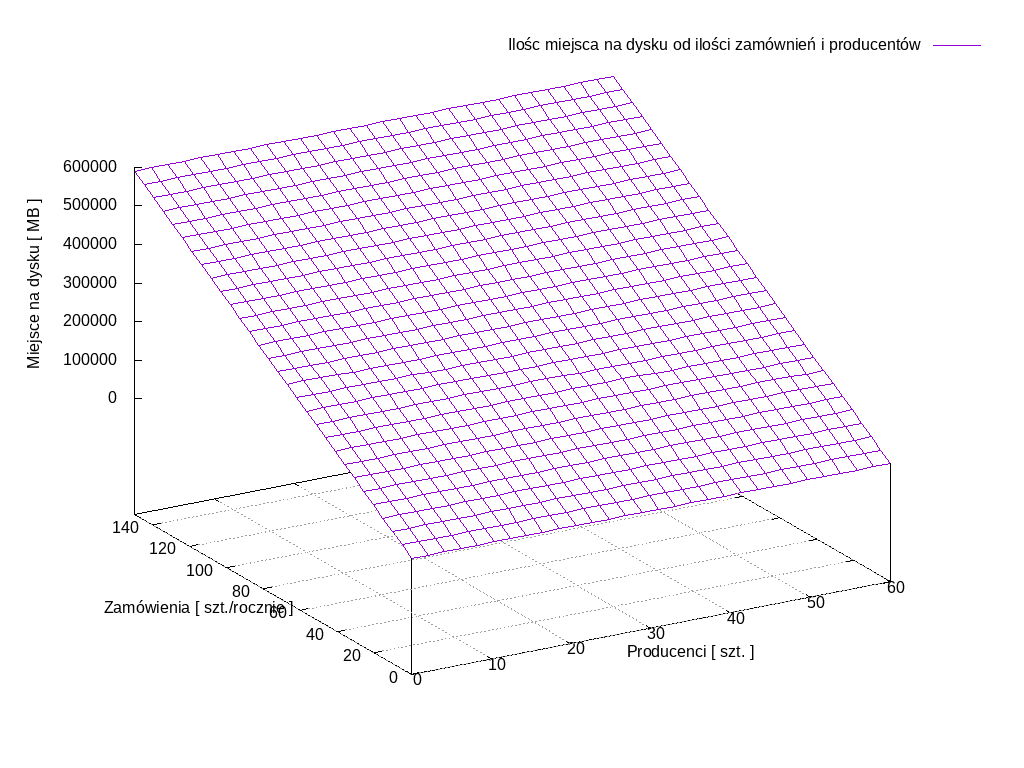
\includegraphics[scale=0.45]{storage}
						\caption{Wykres prezentujący wymaganą pojemność systemu w zależności od ilości producentów i zamówień rocznie}
					\end{figure}
				
					\par Na podstawie przygotowanej funkcji i przeprowadzonej symulacji wynika, że utrzymując około 100 zamówień rocznie i przechowując dane o działaniach z nimi związanych przez okres 5 lat, wymagane jest co najmniej 600GB pamięci. Analiza ta nie uwzględnia ilości danych pochodzących z ochrony bazy danych poprzez technologię PITR.	
 
				
		\subsection{Podsumowanie}
				\par Zaproponowany system komputerowy spełnia pokładane w nim wymagania dotyczące bezpieczeństwa danych, co zostało uzyskane poprzez zastosowanie redundancji danych, mechanizmów ich ochrony i przywracania oraz separacji części użytkowej od rozwojowej systemu. Udało się dowieść również, że system jest wystarczająco pojemny, aby zapewnić wymagane przechowywanie dokumentów skarbowych, eksportowych jak i rejestrację zdarzeń gospodarczych. Jest również odpowiednio wydajny by zapewnić przetwarzanie danych w odpowiednim czasie zarówno dla klienta jak i pracowników sklepu. Co najważniejsze udało się osiągnąć również wysoką niezawodność 96.76\% w okresie 3 lat, która gwarantuje bezpieczne i niezachwiane przetwarzanie informacji.
 


	
	
	
	\section{Opis stanowiska pracy}
			
	Do zadań pracownika należą prace związane z pozyskaniem nowych klientów i producentów, oraz obsługą procesów zamówień i reklamacji. Na pozyskanie klienta składać się będzie: zarządzanie ogłoszeniami na stronie internetowej, portalach aukcyjnych i społecznościowych. Pozyskanie producentów opierać się będzie o próby kontaktu z nowymi zakładami i zdobyciu ich katalogu produktów.
	
\subsection{Urządzenia} 
	Na stanowisko pracy składać się będzie komputer umożliwiający obsługę internetu, poczty elektronicznej, systemu zarządzania firmą czy sklepu internetowego. Drugim narzędziem będzie telefon komórkowy z internetem umożliwiający dzwonienie przez firmową centralę telefoniczną oraz dający dostęp do tych samych funkcji co komputer. Konieczne jest również posiadanie drukarki celem drukowania faktur, zleceń przewozu oraz innych dokumentów. W skład stanowiska musi wchodzić również kasa fiskalna aby rejestrować sprzedaż detaliczną. Jednym z podstawowych narzędzi mojej pracy będzie komputer. Na dzień dzisiejszy posiadam własnego laptopa, którego parametry w początkowej fazie prowadzenia działalności wystarczą.
 
			 
		
	\section{Specyfikacja sprzętu}
        	\subsection{Specyfikacja serwera}
            		\begin{center}
    \begin{longtabu} to \textwidth {|l|l|l|p{0.55\textwidth}|}
        \caption{Specyfikacja techniczna.} \label{tab:long} \\

        \hline 
        \# & Nazwa & Sztuk & Specyfikacja\\ \hline 
        \endfirsthead

        \multicolumn{4}{c}%
        {{\bfseries \tablename\ \thetable{} -- kontynuacja tabeli ze strony poprzedniej}} \\
        \hline
        \# & Nazwa & Specyfikacja & Sztuk\\ \hline 
        \endhead

        \hline \multicolumn{4}{|r|}{{kontynuacja tabeli na stronie następnej}} \\ \hline
        \endfoot

        \hline
        \endlastfoot

        \hline
        \rownumber. & Procesor         &   1    & 
                                                    \begin{description}
                                                        \item[\textbf{Typ procesora:}] Intel Xeon
                                                        \item[\textbf{model procesora:}] E5-2609 v4
                                                        \item[\textbf{typ gniazda:}] Socket 2011-v3
                                                        \item[\textbf{ilość rdzeni:}] 8 szt.
                                                        \item[\textbf{proces technologiczny:}] 14
                                                        \item[\textbf{częstotliwość taktowania procesora:}] 1700 MHz
                                                        \item[\textbf{pojemność pamięci cache:}] L3 20 MB
                                                        \item[\textbf{maksymalny pobór mocy:}] 85 W
                                                    \end{description}   \\ \hline
                                                
        \rownumber. & Płyta główna    &  1      &
                                                    \begin{description}
                                                        \item[\textbf{Złącze karty graficznej:}] PCI Express
                                                        \item[\textbf{Rodzaj pamięć:}] DDR4
                                                        \item[\textbf{Częstotliwość magistrali:}] pamięci 3333 MHz
                                                        \item[\textbf{Częstotliwość magistrali:}] FSB 1366 MHz
                                                        \item[\textbf{Maksymalna wielkość pamięci:}] 128 GB
                                                        \item[\textbf{Format:}] ATX
                                                        \item[\textbf{Karta LAN:}] Intel I218 Gigabit LAN
                                                    \end{description}   \\ \hline
                                                
        \rownumber. & Pamięć RAM     &  1       &
                                                    \begin{description}
                                                        \item[\textbf{Pojemność:}] 32GB
                                                        \item[\textbf{Typ pamięci:}] DDR4
                                                        \item[\textbf{Standard:}] PC4-24000,3000 MHz
                                                        \item[\textbf{Timingi:}] 15-15-15-35-2N
                                                        \item[\textbf{Napięcie:}] 1.35 V
                                                        \item[\textbf{Radiator:}] Tak
                                                    \end{description}     \\ \hline
                                                
        \rownumber. & Dysk twardy   &  1        &   
                                                    \begin{description}
                                                        \item[\textbf{Pojemność:}]120 GB
                                                        \item[\textbf{interfejs:Serial ATA III}]
                                                        \item[\textbf{Prędkość odczytu:}] 550 MB/s
                                                        \item[\textbf{Prędkość zapisu:}]540 MB/s KontrolerPhison S11
                                                        \item[\textbf{Losowy odczyt danych:}] 4K85000 IOPS
                                                        \item[\textbf{Losowy zapis danych:}] 4K81000 IOPSOMb/s
                                                        \item[\textbf{Zapis danych niekompresowalnych:}] 450 Mb/s
                                                    \end{description}            \\ \hline
                                                
        \rownumber. & Zasilacz     &  1         &
                                                    \begin{description}
                                                        \item[\textbf{Moc:}]600 W
                                                        \item[\textbf{Standard:}]ATX
                                                        \item[\textbf{Głośność maksymalna:}]20,3 dB
                                                        \item[\textbf{Głośność minimalna:}]11,2 dB
                                                        \item[\textbf{Waga:}]2,15 kg
                                                        \item[\textbf{Certyfikat sprawności:}] 80Plus Silver
                                                    \end{description}         \\ \hline
                                            
        \rownumber. & Obudowa    &   1          &  
                                                    \begin{description}
                                                        \item[\textbf{Format płyty główne:}] ATX, microATX
                                                        \item[\textbf{Wysokość:}] 475 mm
                                                        \item[\textbf{Długość:}] 435 mm
                                                        \item[\textbf{Szerokość:}] 200 mm
                                                        \item[\textbf{Waga obudowy:}] 4,3 kg
                                                    \end{description}\\ \hline
    \end{longtabu}
\end{center}

%    \end{tabular}
%    \caption{Specyfikacja sprzętowa serwera}
%    \label{my-label}
%\end{table}


		\subsection{Specyfikacja dysku sieciowego}	
			\begin{center}
    \begin{longtabu} to \textwidth {|l|l|l|p{0.75\textwidth}|}
        \caption{Specyfikacja techniczna.} \label{tab:long} \\

        \hline 
        \# & Nazwa & Sztuk & Specyfikacja\\ \hline 
        \endfirsthead

        \multicolumn{4}{c}%
        {{\bfseries \tablename\ \thetable{} -- kontynuacja tabeli ze strony poprzedniej}} \\
        \hline
        \# & Nazwa & Specyfikacja & Sztuk\\ \hline 
        \endhead

        \hline \multicolumn{4}{|r|}{{kontynuacja tabeli na stronie następnej}} \\ \hline
        \endfoot

        \hline
        \endlastfoot
        
        \hline

        \rownumber. & Procesor         &   1        & 
                                                        \begin{description}
                                                            \item[\textbf{Typ procesora:}] Intel Core
                                                            \item[\textbf{model procesora:}] i3-7300
                                                            \item[\textbf{typ gniazda:}] Socket 1151
                                                            \item[\textbf{ilość rdzeni:}] 4 szt.
                                                            \item[\textbf{proces technologiczny:}] 14
                                                            \item[\textbf{częstotliwość taktowania procesora:}] 4000 MHz
                                                            \item[\textbf{pojemność pamięci cache:}] L3 4 MB
                                                            \item[\textbf{maksymalny pobór mocy:}] 85 W
                                                        \end{description}
                                                      \\ \hline
                                                
        \rownumber. & Płyta główna      &  1        &
                                                        \begin{description}
                                                            \item[\textbf{Złącze karty graficznej:}] PCI Express
                                                            \item[\textbf{Rodzaj pamięć:}] DDR4
                                                            \item[\textbf{Częstotliwość magistrali:}] pamięci 2400 MHz
                                                            \item[\textbf{Częstotliwość magistrali:}] FSB 1167 MHz
                                                            \item[\textbf{Maksymalna wielkość pamięci:}] 64 GB
                                                            \item[\textbf{Format:}] ATX
                                                            \item[\textbf{Karta LAN:}] Intel I218 Gigabit LAN
                                                        \end{description}
                                                     \\ \hline
                                                
        \rownumber. & Pamięć RAM        &  1        &
                                                        \begin{description}
                                                            \item[\textbf{Model:}] Ripjaws V
                                                            \item[\textbf{Pojemność:}] 8GB
                                                            \item[\textbf{Typ pamięci:}] DDR4
                                                            \item[\textbf{Standard:}] PC4-24000, 3000 MHz
                                                            \item[\textbf{Timingi:}] 15-15-15-35-2N
                                                            \item[\textbf{Napięcie:}] 1.35 V
                                                        \end{description}
                                                     \\ \hline
                                                
        \rownumber. & Dysk twardy (SSD) &  1        &   
                                                        \begin{description}
                                                            \item[\textbf{Pojemność:}]120 GB
                                                            \item[\textbf{interfejs:Serial ATA III}]
                                                            \item[\textbf{Prędkość odczytu:}] 550 MB/s
                                                            \item[\textbf{Prędkość zapisu:}]540 MB/s KontrolerPhison S11
                                                            \item[\textbf{Losowy odczyt danych:}] 4K85000 IOPS
                                                            \item[\textbf{Losowy zapis danych:}] 4K81000 IOPSOMb/s
                                                            \item[\textbf{Zapis danych niekompresowalnych:}] 450 Mb/s
                                                        \end{description}            \\ \hline

        \rownumber. & Dysk twardy (HDD) &   2       & 
                                                        \begin{description}
                                                            \item[\textbf{Model:}] Format:3,5 cali
                                                            \item[\textbf{Pojemność:}] 2000 GB
                                                            \item[\textbf{InterfejsSerial ATA III}]
                                                            \item[\textbf{Prędkość odczytu:}] 550 MB/s
                                                            \item[\textbf{Prędkość zapisu:}] 540 MB/s KontrolerPhison S11
                                                            \item[\textbf{Losowy odczyt danych:}] 4K85000 IOPS
                                                            \item[\textbf{Losowy zapis danych:}] 4K81000 IOPSOMb/s
                                                            \item[\textbf{Zapis danych niekompresowalnych:}]450 Mb/s
                                                        \end{description} \\ \hline
                                                        
        \rownumber. & Zasilacz          &  1         &
                                                        \begin{description}
                                                            \item[\textbf{Moc:}]600 W
                                                            \item[\textbf{Standard:}]ATX
                                                            \item[\textbf{Głośność maksymalna:}]20,3 dB
                                                            \item[\textbf{Głośność minimalna:}]11,2 dB
                                                            \item[\textbf{Waga:}]2,15 kg
                                                            \item[\textbf{Certyfikat sprawności:}] 80Plus Silver
                                                        \end{description}         \\ \hline
                                            
        \rownumber. & Obudowa    &   1          &  
                                                        \begin{description}
                                                            \item[\textbf{Format płyty główne:}] ATX, microATX
                                                            \item[\textbf{Wysokość:}] 475 mm
                                                            \item[\textbf{Długość:}] 435 mm
                                                            \item[\textbf{Szerokość:}] 200 mm
                                                            \item[\textbf{Waga obudowy:}] 4,3 kg
                                                        \end{description}\\ \hline
    \end{longtabu}
    %\caption{Specyfikacja macierz dyskowa}
    %\label{my-label}
\end{center} 

			
		\subsection{Specyfikacja zbiorcza}	
			\begin{center}
\begin{longtabu} to \textwidth {|l|p{0.25\textwidth}|p{0.7\textwidth}|l|}
\caption{Specyfikacja techniczna.} \label{tab:long} \\

\hline 
\# & Nazwa & Specyfikacja & Sztuk\\ \hline 
\endfirsthead

\multicolumn{4}{c}%
{{\bfseries \tablename\ \thetable{} -- kontynuacja tabeli ze strony poprzedniej}} \\
\hline
\# & Nazwa & Specyfikacja & Sztuk\\ \hline 
\endhead

\hline \multicolumn{4}{|r|}{{kontynuacja tabeli na stronie następnej}} \\ \hline
\endfoot

\hline
\endlastfoot

\rownumber 	& Procesor serwerowy 	& 	Część serwera, niezbędny do przetwarzania danych.
												\begin{description}
													\item[\textbf{Typ procesora:}] Intel Xeon
													\item[\textbf{model procesora:}] E5-2609 v4
													\item[\textbf{typ gniazda:}] Socket 2011-v3
													\item[\textbf{ilość rdzeni:}] 8 szt.
													\item[\textbf{proces technologiczny:}] 14
													\item[\textbf{częstotliwość taktowania procesora:}] 1700 MHz
													\item[\textbf{pojemność pamięci cache:}] L3 20 MB
													\item[\textbf{maksymalny pobór mocy:}] 85 W
												\end{description}
												\url{https://www.arest.pl/produkt/52084/INTEL-Xeon-E5-2609-v4-1-70-GHz-x8-8-20-MB-85W-BOX-s-2011-V3/wlasciwosci}
								& 2 \\ \hline

\rownumber 	& Procesor komputerowy 	& 	Część macierzy dyskowej, niezbędny do przetwarzania danych.
												\begin{description}
													\item[\textbf{Typ procesora:}] Intel Core
													\item[\textbf{model procesora:}] i3-7300
													\item[\textbf{typ gniazda:}] Socket 1151
													\item[\textbf{ilość rdzeni:}] 4 szt.
													\item[\textbf{proces technologiczny:}] 14
													\item[\textbf{częstotliwość taktowania procesora:}] 4000 MHz
													\item[\textbf{pojemność pamięci cache:}] L3 4 MB
													\item[\textbf{maksymalny pobór mocy:}] 85 W
												\end{description}
												\url{https://proline.pl/procesor-intel-core-i3-7300-4-0-ghz-s-1151-box-p952159}
								& 2 \\ \hline								
								
\rownumber &  Płyta główna serwerowa		& Część serwera niezbędna do zamontowania na niej
												wewnątrz komputera podstawowych jego elementów.
											\begin{description}
												\item[\textbf{Model:}] MSI X99A GAMING 7 s.2011
												\item[\textbf{Złącze karty graficznej:}] PCI Express
												\item[\textbf{Rodzaj pamięć:}] DDR4
												\item[\textbf{Częstotliwość magistrali:}] pamięci 3333 MHz
												\item[\textbf{Częstotliwość magistrali:}] FSB 1366 MHz
												\item[\textbf{Maksymalna wielkość pamięci:}] 128 GB
												\item[\textbf{Format:}] ATX
												\item[\textbf{Karta LAN:}] Intel I218 Gigabit LAN
											\end{description}
											\url{https://proline.pl/msi-x99a-gaming-7-s-2011-p944535}
								& 2 \\ \hline

\rownumber &  Płyta główna komputerowa		& Część macierzy dyskowej niezbędna do zamontowania na niej
												wewnątrz komputera podstawowych jego elementów.
											\begin{description}
												\item[\textbf{Model:}]Gigabyte GA-Z170-D3H DDR4 1151
												\item[\textbf{Złącze karty graficznej:}] PCI Express
												\item[\textbf{Rodzaj pamięć:}] DDR4
												\item[\textbf{Częstotliwość magistrali:}] pamięci 2400 MHz
												\item[\textbf{Częstotliwość magistrali:}] FSB 1167 MHz
												\item[\textbf{Maksymalna wielkość pamięci:}] 64 GB
												\item[\textbf{Format:}] ATX
												\item[\textbf{Karta LAN:}] Intel I218 Gigabit LAN
											\end{description}
											\url{https://proline.pl/gigabyte-ga-z170-d3h-ddr4-1151-p941062}
								& 2 \\ \hline
								
								
\rownumber &  Pamięć RAM 16GB  	& Część serwera i macierzy dyskowej, niezbędna do przechowywania 
												wykonywanych programów komputerowych i wyników ich przetwarzania. 
												wewnątrz komputera podstawowych jego elementów.
											\begin{description}
												\item[\textbf{Model:}] Ripjaws V
												\item[\textbf{Ilość:}] 2 sztuki
												\item[\textbf{Pojemność:}] 2x 16GB
												\item[\textbf{Typ pamięci:}] DDR4
												\item[\textbf{Standard:}] PC4-24000,3000 MHz
												\item[\textbf{Timingi:}] 15-15-15-35-2N
												\item[\textbf{Napięcie:}] 1.35 V
												\item[\textbf{Radiator:}] Tak
                                            \end{description}
                                            \url{https://www.komputronik.pl/product/306811/g-skill-ripjaws-16gb-1x16gb-2133mhz-ddr4-cl15-sodimm-.html?gclid=Cj0KCQjwy4zLBRCOARIsADfss35QpYiAKWGkPFBjym7ZBfUZeH5KrIXaDe_oNqqp7CjyW0SKoWlKVlkaAjnfEALw_wcB&gclsrc=aw.ds}
										&	2		\\ \hline

\rownumber &  Pamięć RAM 8GB 		& Część serwera i macierzy dyskowej, niezbędna do przechowywania 
												wykonywanych programów komputerowych i wyników ich przetwarzania. 
												wewnątrz komputera podstawowych jego elementów.
											\begin{description}
												\item[\textbf{Model:}] Ripjaws V
												\item[\textbf{Pojemność:}] 8GB
												\item[\textbf{Typ pamięci:}] DDR4
												\item[\textbf{Standard:}] PC4-24000, 3000 MHz
												\item[\textbf{Timingi:}] 15-15-15-35-2N
												\item[\textbf{Napięcie:}] 1.35 V
                                            \end{description}
                                            \url{https://www.morele.net/pamiec-g-skill-ripjaws-v-ddr4-16gb-8gbx2-3200mhz-cl16-1-35v-f4-3200c16d-16gvk-707300/}
										& 3 \\ \hline	
								
\rownumber &  Dysk NAS 2TB  	& Część macierzy dyskowej, umożliwiający zapisywanie danych. Posiada 5-letnią gwarancje.
												Jest to dysk przystosowany do wielogodzinnej pracy. 
											\begin{description}
												\item[\textbf{Model:}] WD Red WD20EFRX
												\item[\textbf{Format:}] 3,5 cala
												\item[\textbf{Pojemność:}] 2000 GB
												\item[\textbf{InterfejsSerial ATA III}]
												\item[\textbf{Prędkość odczytu:}] 550 MB/s
												\item[\textbf{Prędkość zapisu:}] 540 MB/s KontrolerPhison S11
												\item[\textbf{Losowy odczyt danych:}] 4K85000 IOPS
												\item[\textbf{Losowy zapis danych:}] 4K81000 IOPSOMb/s
												\item[\textbf{Zapis danych niekompresowalnych:}]450 Mb/s
										\end{description}												
										\url{https://proline.pl/dysk-wd-red-wd20efrx-2tb-sata-iii-64mb-p924806}
										&	4		\\ \hline
												
											
												

\rownumber &  Dysk SSD 		& Część serwera i macierzy dyskowej, niezbędny do przechowywania systemu operacyjnego.
											\begin{description}
												\item[\textbf{Pojemność:}]120 GB
												\item[\textbf{interfejs:Serial ATA III}]
												\item[\textbf{Prędkość odczytu:}] 550 MB/s
												\item[\textbf{Prędkość zapisu:}]540 MB/s KontrolerPhison S11
												\item[\textbf{Losowy odczyt danych:}] 4K85000 IOPS
												\item[\textbf{Losowy zapis danych:}] 4K81000 IOPSOMb/s
												\item[\textbf{Zapis danych niekompresowalnych:}] 450 Mb/s
                                            \end{description}														
                                            \url{https://proline.pl/goodram-ssd-cx300-2-5-cali-120gb-ssdpr-cx300-120-p948141}
										& 4 \\ \hline	
										
\rownumber &  Zasilacz 		& Część serwera i macierzy dyskowej, element elektromechaniczny dostarczający prąd do pozostałych komponentów komputera.
											\begin{description}
												\item[\textbf{Moc:}]600 W
												\item[\textbf{Standard:}]ATX
												\item[\textbf{Głośność maksymalna:}]20,3 dB
												\item[\textbf{Głośność minimalna:}]11,2 dB
												\item[\textbf{Waga:}]2,15 kg
												\item[\textbf{Certyfikat sprawności:}] 80Plus Silver
										\end{description}
										\url{https://proline.pl/zasilacz-be-quiet-pure-power-10-600w-cm-p950048}
										& 4 \\ \hline											


\rownumber &  Obudowa 		& Część serwera i macierzy dyskowej, niezbędna do umieszczenia w nim wszystkich komponentów komputera.
											\begin{description}
												\item[\textbf{Format płyty główne:}] ATX, microATX
												\item[\textbf{Wysokość:}] 475 mm
												\item[\textbf{Długość:}] 435 mm
												\item[\textbf{Szerokość:}] 200 mm
												\item[\textbf{Waga obudowy:}] 4,3 kg
										\end{description}												
										\url{https://proline.pl/obudowa-cyclone-rage-r75-pure-black-p947401}
										& 4 \\ \hline
										

\rownumber &  Drukarka sieciowa 		
				wielofunkcyjna	& Niezbędna do szybkiego drukowania, skanowania, kserowania wszelkich dokumentów.
										\begin{description}
												\item[\textbf{Technologia druku:}] Laserowa kolorowa
												\item[\textbf{Szybkość druku:}] 26 ston na minute
												\item[\textbf{Typ skanera:}] Płaski
												\item[\textbf{Rozdzielczość skanera:}] 1200 x 1200 dpi
												\item[\textbf{Głębia koloru:}] 24 bit
												\item[\textbf{Rozdzielczość kopiarki:}] 600 x 600 dpi
												\item[\textbf{Pojemność pamięci faksu:}] 200 stron
												\item[\textbf{Szybkość transmisji faksu:}] 33.6 kbps
												\item[\textbf{Szerokość:}] 427 mm
												\item[\textbf{Głębokość:}] 509 mm
												\item[\textbf{Wysokość:}] 444 mm
												\item[\textbf{Waga:}] 29 kg
												\item[\textbf{Normatywne obciążenie:}] 5000 str./mies. 
										\end{description}											
										\url{https://www.usa.canon.com/internet/portal/us/home/products/details/printers/color-laser/color-imageclass-mf731cdw}
										& 1 \\ \hline	
										
\rownumber & Kasa fiskalna 
				walutowa			& Zgodnie z przepisami potrzebna do prowadzenia działalności gospodarczej.
											Ze względu na działalność międzynarodową kasa walutowa jest 
											niezbędnym narzędziem pracy.
										\begin{description}
												\item[\textbf{Ilość PLU:}] Bez ograniczeń
												\item[\textbf{Grupy towarowe:}] Bez ograniczeń
												\item[\textbf{Nazwa towaru:}] 40 znaków
												\item[\textbf{Ilość kasjerów:}] Bez ograniczeń
												\item[\textbf{Stawki PTU:}] 7
												\item[\textbf{Ilość pozycji na paragonie:}] 255
												\item[\textbf{Kasa walutowa:}] Tak
												\item[\textbf{Elektroniczna kopia:}] Karta USD
												\item[\textbf{Szerokość papieru:}] 57 mm
												\item[\textbf{Wyświetlacz:}] Ekran TTFT kolorowy 7 cali, 800x480 piksele
												\item[\textbf{Zasilacz:}] 230V/12V/2A
												\item[\textbf{Akumulator:}] 6V, 3Ah(40000 wierszy, 2500 paragonów)
												\item[\textbf{Szerokość:}] 262 mm
												\item[\textbf{Głębokość:}] 242 mm
												\item[\textbf{Wysokość:}] 96 mm
												\item[\textbf{Praca On-line z komputerem:}] Tak
												\item[\textbf{NIP nabywcy na paragonie:}] Tak
												\item[\textbf{Obsługa DHCP:}] Tak
												\item[\textbf{Funkcja sprawdzarki cen:}] Tak
										\end{description}									
										\url{http://www.voipsklep.pl/INCOM-ICW1000G_607_2.html}
										& 1 \\ \hline										
										
\rownumber &  Access Point 
                                    & Inaczej router bezprzewodowy, umożliwia podłączenie do sieci urządzeń bezprzewodowych: laptop, telefon
										\begin{description}
												\item[\textbf{Funkcje:}] Router
												\item[\textbf{Typ złącza:}] Ethernet
												\item[\textbf{Protokół Wi-Fi:}] 802,11b/g/n/ac
										\end{description}												
										\url{https://proline.pl/tp-link-archer-c60-ac1350-wireless-dual-band-router-p949040}
										& 1 \\ \hline
										
\rownumber & Karta graficzna 		
									& Część serwera i macierzy dyskowej, przede wszystkim do wyświetlenia obrazu, niezbędna podczas wstępnej konfiguracji
										\begin{description}
												\item[\textbf{Typ złącza:}] PCI-Express 2,0 x16
												\item[\textbf{Typ pamięci:}] DDR3
												\item[\textbf{Szyna pamięci:}] 64 bit
												\item[\textbf{Pamięć:}] 1024 MB
												\item[\textbf{Maksymalna rozdzielczość:}] 2560x1600
												\item[\textbf{Częstotliwość rdzenia:}] 589 MHz
												\item[\textbf{Częstotliwość RAMDAC:}] 400 MHz
												\item[\textbf{Częstotliwość pamięci:}] 1000 MHz
												\item[\textbf{Chipset producent:}] NVIDIA
												\item[\textbf{Wymiary:}] 145 x 84 x 18 cm
												\url{https://proline.pl/?p=N210-MD1GD3H\%2FLP}
											\end{description}			
										
										& 3 \\ \hline										

										
\rownumber & Switch			& Szesnasto portowy przełącznik umożliwiający obsługę gigabitowego połączenia Ethernet
										\begin{description}
												\item[\textbf{Szybkość łącza:}] 1 Gbps
												\item[\textbf{Liczba portów:}] 16
												\item[\textbf{Typ złącza:}] Ethernet
												\item[\textbf{Wymiary:}] 294 x 180 x 44 cm
											\end{description}
											\url{https://proline.pl/tp-link-tl-sg1016d-switch-16x10-100-1000mbps-p932369}
											& 1 \\ \hline		
											
\rownumber & Telefon VOIP & 

\end{longtabu}
\end{center}
 


	%\section{TEN GANTT to CHYBA MARKETINGOWY}
	%		\includepdf[pages={1-},scale=0.75]{sklep-meblowy-org-gantt.pdf}
		
   %\subsubsection{Analiza kosztów utrzymania}
	%\par Na koszty utrzymania systemu składać się będą koszty prądu oraz koszty usług telekomunikacyjnych. Jako koszty telekomunikacyjne rozumiane są wydatki na łącze internetowe, oraz abonament za dwa numery telefoniczne polski i kanadyjski.
		
			\paragraph{Koszty prądu}
				\par Koszty prądu można wyliczyć posługując się danymi ze specyfikacji technicznej sprzętu komputerowego. Zużycie prądu w watach przedstawia poniższa lista:

				\begin{itemize}
					\item{Procesor serwerowy} 85W
			 
                    \item{Procesor komputerowy} 55W
			 
					\item{Płyta główna serwerowa} 70W
			
                    \item{Płyta główna komputerowa} 45W
			
					\item{Pamięć operacyjna} 4W
			
					\item{Dysk twardy HDD} 8W
			
					\item{Dysk twardy SSD} 3W
			
					\item{Karta graficzna} 15W
				\end{itemize}

				\par Co po przemnożeniu przez ilość elementów określonych w wycenie daje:
				
				\begin{itemize}
					\item{Procesor} 280W
			 
					\item{Płyta główna} 230W
			
					\item{Pamięć operacyjna} 24W
			
					\item{Dysk twardy HDD} 32W
			
					\item{Dysk twardy SSD} 9W
			
					\item{Karta graficzna} 45W
				\end{itemize}
				
				\par Daje to sumaryczne zużycie prądu przez sprzęt komputerowy 620W. Należy wziąć tu jeszcze pod uwagę sprawność zasilacza, która dla wybranego modelu wynosi ok. 80\%. Znaczy to, że sprzęt komputerowy poprzez straty na zasilaczu będzie pobierał 20\% energii więcej co daje około 744W. Wliczając w to pobór prądu przez urządzenia takie jak kasa fiskalna, router, drukarka, switch daje ok 800W, Biorąc pod uwagę pracę systemu 24 godziny na dobę przez cały rok daje zużycie energii na poziomie 7000 kWh rocznie. Do tych kosztów należy doliczyć jeszcze energię zużytą przez komputer na stanowisku pracowniczym pracujący 8 godzin dziennie przez 250 dni, (tyle bowiem średnio jest dni pracujących w roku) pobierający około 80W energii na godzinę. Daje to zużycie prądu rocznie na poziomie 160 kWh. Na tej podstawie można oszacować średnie roczne zużycie prądu 7150 kWh. Czyli w ujęciu miesięcznym 595 kWh, co biorąc pod uwagę średni koszt kWh prądu na Dolnym Śląsku około 0.55 zł/kWh daje szacunkowo 320zł/m-c. Zakładając 5\% niedoszacowanie wartości wychodzi około 340zł/m-c. Odchylenie to wynika z szacowania poboru prądu dla urządzeń w stanie pracy bez obciążenia. Nie będzie to już w tym wypadku wartość znacząca jednak warto o pamiętać o tym fakcie.

			\paragraph{Koszty telekomunikacyjne}
				\par Do kosztów telekomunikacyjnych należy wliczyć koszt utrzymania połączenia internetowego, ze względu na konieczność utrzymywania dwóch adresów IP co wynika wprost z rfc1035, określającego parametry łączą dla przechowywania domeny, daje 110zł/m-c. Dla łączą o parametrach 2 x 100/100Mbps. Do kosztów tych należy doliczyć jeszcze koszt dwóch numerów w Polsce i Kanadzie z nielimitowanym planem taryfowym 70zł/m-c przy wykorzystaniu technologii VOIP (Voice Over IP).
		
			\paragraph{Porównanie kosztów}
				\par Koszty prądu na same tylko 3 serwery wynoszą około 280 zł/m-c doliczając do tego koszt łącza internetowego w wysokości 110zł/m-c otrzymujemy 390zł miesięcznie  dla porównania w tej samej cenie możemy np. w serwerowniach takich jak ovh.pl czy home.pl wynająć jeden 4 rdzeniowy komputer z 1 terabajtowym dyskiem twardym. Wynajęcie równoważnej infrastruktury to koszt około 1500zł/m-c. Co przemawia stanowczo za utworzeniem własnego zaplecza technicznego. 
 

							
	\subsection{Wycena inwestycji}
	 	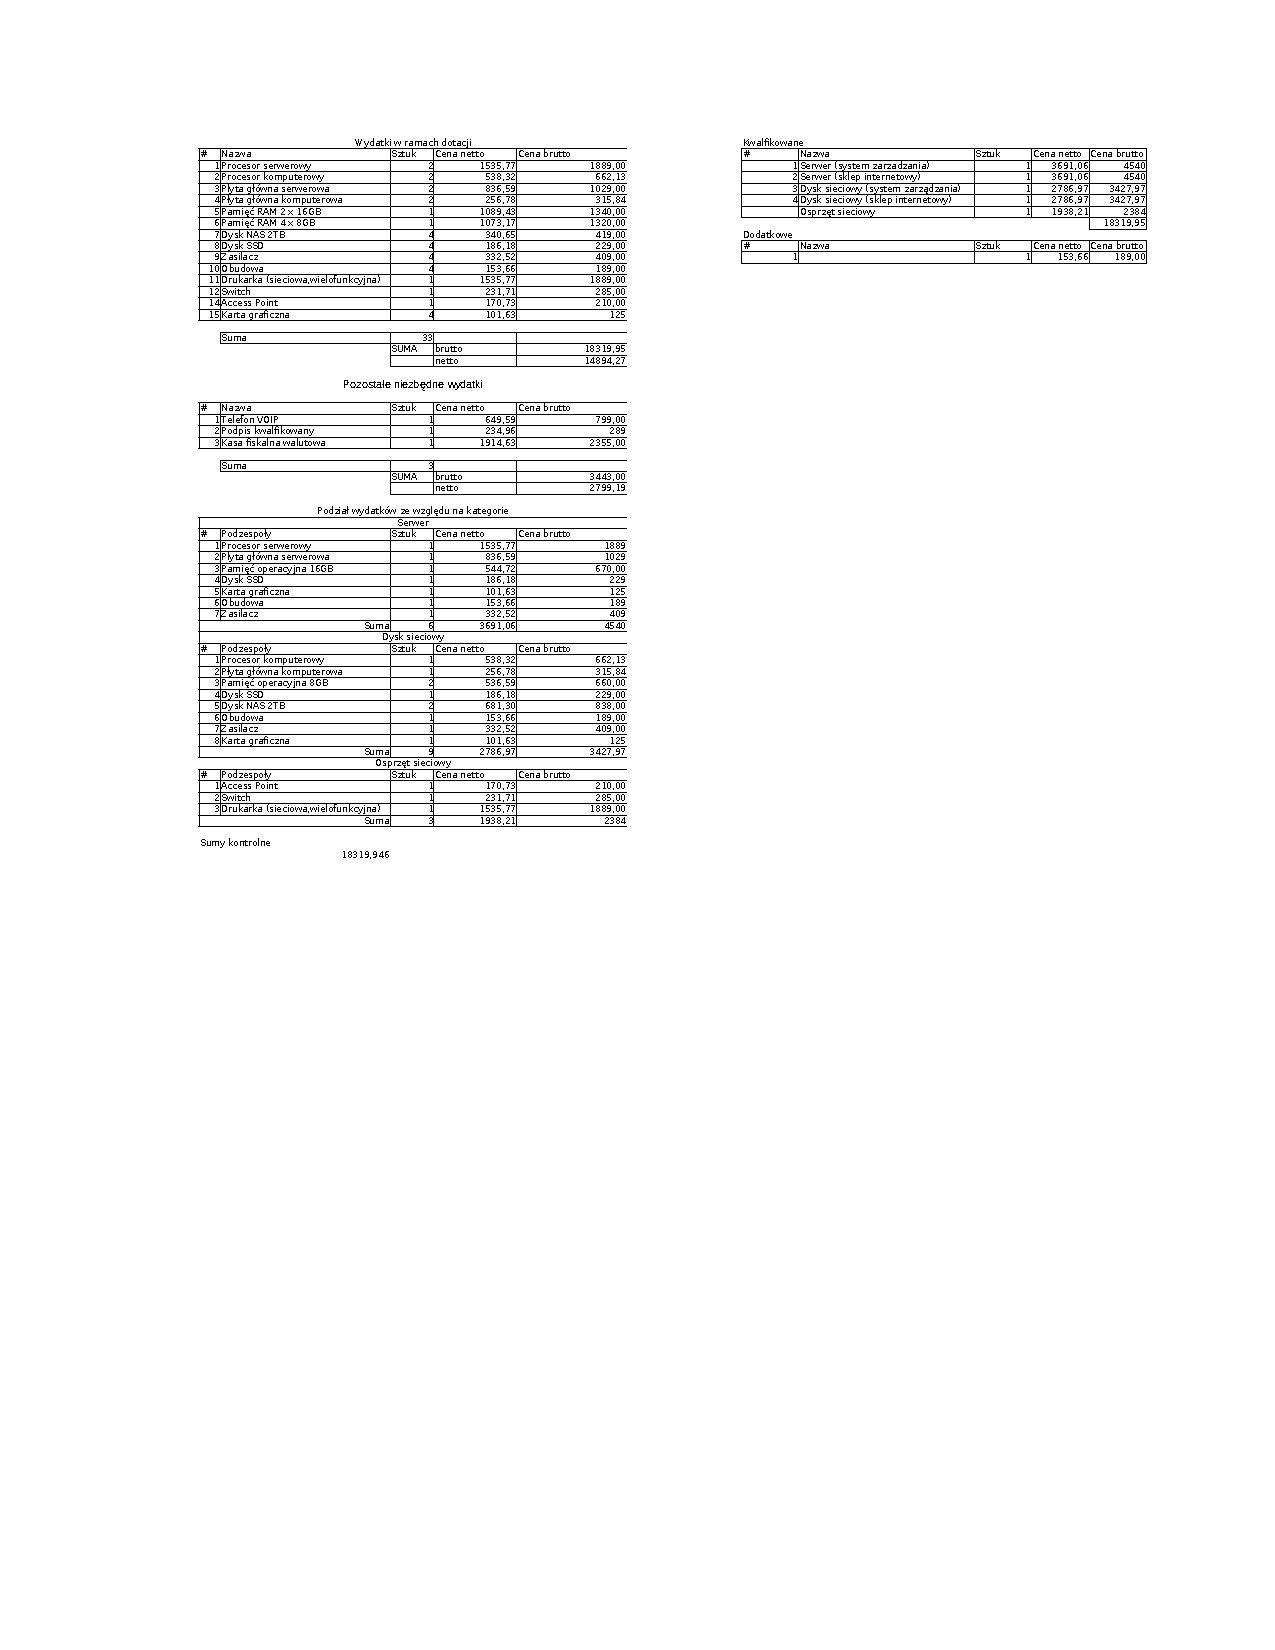
\includepdf[pages={1-},width=\textwidth]{wycena.pdf}

		

	
	\chapter{Plan finansowy}
		\section{Źródła finansowania}
				\subsection{Wstęp}
		\par Przed założeniem własnej firmy, każdy przyszły przedsiębiorca musi zdobyć środki finansowe na jej funkcjonowanie. Sposób pozyskiwania tych środków zależy od wielkości firmy, wzrostu, etapu jej rozwoju. Źródła finansowania przedsiębiorstwa są różne. Może być to nasz własny kapitał albo kapitał obcy. Jeden i drugi ma swoje plusy i minusy. Wkład własny jest z jednej strony najbezpieczniejszy, ale najczęściej jest bardzo niski. Kapitał obcy czyli leasing, kredyty bankowe, dotacje i subwencje itp., zawsze trzeba zwrócić.
		
	\subsection{Źródła finansowania przedsiębiorstwa}
		\par Do prowadzenia sklepu internetowego potrzebuję właściwego oprogramowania oraz platformy sprzętowej, które zapewnią mi prowadzenie działalności na najwyższym poziomie. Dużym nacisk kładę na bezpieczeństwo zarówno sklepu jak i klientów.
		
		\par Do sfinansowania tego przedsięwzięcia potrzebne są mi środki finansowe, które umożliwią mi zakup drogiego sprzętu komputerowego. Głównym źródłem finansowania będzie tu dotacja ze środków unijnych w ramach projektu "Akademia przedsiębiorczości kobiet"". Pełna kwota dotacji to 24000 zł dofinansowania jednorazowego. Dodatkowo mogę otrzymać comiesięczne wsparcie pomostowe w wysokości 1350 zł na pokrycie codziennych kosztów związanych z prowadzeniem działalności.
		
		\par Posiadam również kapitał własny w wysokości 8 tysięcy złotych, które mogę przeznaczyć na reklamę, zakup mebli biurowych itp. ,oraz własnego laptopa niezbędnego do prowadzenia sklepu internetowego o wartości 2200 zł. 
		
		\par Warto również zaznaczyć, że posiadam drogie narzędzia programowe, gwarantujące przede wszystkim niezależność, bezpieczeństwo sklepu jak i klientów, oraz nienaganne działanie platformy. Są to:
		
		\begin{itemize}
		
			\item Oprogramowanie sklepu internetowego bazujące na platformie Drupal
				
			\item Oprogramowanie serwera stron internetowych
				
			\item Oprogramowanie serwera wiadomości e-mail
				
			\item Centrala telefoniczna PBX
				
			\item System zarządzania bazujący na platformie Redmine
				
				
		\end{itemize}	
				
				
				\par W prognozie na 3 lata uwzględniłam również zatrudnienie pracowników. Mogę to zrobić poprzez urząd pracy, a tym samym starać się o wsparcie finansowe, związane z tym zatrudnieniem. Mogę starać się o dofinansowanie wynagrodzenia nowo zatrudnionego, jego składek ubezpieczenia społecznego, jak również refundację doposażenia jego stanowiska pracy. Takie działanie przynosi obustronne korzyści- osoby bezrobotne mają szanse na dobrą pracę, a ja jako pracodawca zminimalizuje koszty związane z zatrudnieniem nowego pracownika.	

		\section{Koszty miesięczne}
			\subsection{Charakterystyka}

	\begin{enumerate}
		\item{\textbf{Zakup towarów}} - koszt zakupu towaru przez klientów.
		
		\item{\textbf{Ubezpieczenia rzeczowe}} - są to niezbędne ubezpieczenia sprzętu komputerowego.
		
		\item{\textbf{Koszty administracyjne }}
			\begin{enumerate}
				
				\item{\textbf{Reklama}} - koszty związane z pozycjonowaniem strony, reklamie internetowej, kolportażu ulotek, które pozwolą na promowanie mojego sklepu.
				
					\begin{enumerate}
					
						\item{\textbf{Kolportaż ulotek}} - koszty związane z kupnem i drukowaniem ulotek 
		
						\item{\textbf{Bilbord}} - koszty związane z wynajęciem bilbordu
					
					\end{enumerate}
					
				\item{\textbf{Wynagrodzenie pracowników}} - koszt wynikający z planowanego zatrudnienia w drugim i trzecim roku prowadzenia działalności.
			
				\item{\textbf{Narzuty wynagrodzenia}} - są to wszystkie obowiązkowe obciążenia narzucone na pracodawcę z tytułu zatrudnienia pracowników. Są to: składki z tytułu ubezpieczenie społecznego, składki na Fundusz Pracy i Fundusz Gwarantowanych Świadczeń Pracowniczych, odpisy na Zakładowy Fundusz Świadczeń Socjalnych.
			
				\item{\textbf{Energia}} - na koszty utrzymania systemu składać się będą koszty prądu.
					\begin{enumerate}
						
						\item{\textbf{Prąd}} - koszty powstałe na skutek wykorzystania systemu komputerowego \label{prad}
						
						\item{\textbf{Ogrzewanie}} - koszty powstałe na skutek ogrzewania obiektu 
						
					\end{enumerate}
					
				\item{\textbf{Usługi obce}} - zostały tu ujęte usługi księgowe, których szacowany koszt miesięczny wynosi 200 zł.
			
				\item{\textbf{Podatki lokalne}} - podatek od powierzchni, na której będę prowadzić działalności.

				\item{\textbf{inne koszty}} składka na ubezpieczenie  społeczne  właściciela.
			
				\item{\textbf{Koszty telekomunikacyjne}} - Do kosztów telekomunikacyjnych należy wliczyć koszt utrzymania połączenia internetowego, ze względu na konieczność utrzymywania dwóch adresów IP co wynika wprost z rfc1035, określającego parametry łączą dla przechowywania domeny, daje 110zł/m-c. Dla łączą o parametrach 2 x 100/100Mbps. Do kosztów tych należy doliczyć jeszcze koszt dwóch numerów w Polsce i Kanadzie z nielimitowanym planem taryfowym 70zł/m-c przy wykorzystaniu technologii VOIP (Voice Over IP).
		
				%\item Amortyzacja - koszt związany ze stopniowym zużywaniem się środków trwałych i wartości niematerialnych i prawnych. Dokonałam jednorazowej amortyzacji na kwotę 5667 zł.- pomoc de minimis. Dotyczy ona zakupu procesorów serwerowych.
			\end{enumerate}
				
	\end{enumerate}		

			
		\paragraph{Koszty prądu-uzasadnienie \cref{prad}}		
			
			
	\par Koszty prądu można wyliczyć posługując się danymi ze specyfikacji technicznej sprzętu komputerowego. Zużycie prądu w watach przedstawia poniższa lista:
	
			\begin{itemize}
				\item{\textbf{Procesor}} - 85W
					
				\item{\textbf{Płyta główna}} - 70W
					
				\item{\textbf{Pamięć operacyjna}} - 4W
					
				\item{\textbf{Dysk twardy HDD}} - 8W
					
				\item{\textbf{Dysk twardy SSD}} - 3W
					
				\item{\textbf{Karta graficzna}} - 15W
			\end{itemize}

			\par Co po przemnożeniu przez ilość elementów określonych w wycenie daje:
						
			\begin{itemize}
				\item{\textbf{Procesor}} - 255W
					
				\item{\textbf{Płyta główna}} - 210W
					
				\item{\textbf{Pamięć operacyjna}} - 24W
					
				\item{\textbf{Dysk twardy HDD}} - 32W
					
				\item{\textbf{Dysk twardy SSD}} - 9W
					
				\item{\textbf{Karta graficzna}} - 45W
			\end{itemize}
				
		\par Daje to sumaryczne zużycie prądu przez sprzęt komputerowy 575W. Należy wziąć tu jeszcze pod uwagę sprawność zasilacza, która dla wybranego modelu wynosi ok. 80\%. Znaczy to, że sprzęt komputerowy poprzez straty na zasilaczu będzie pobierał 20\% energii więcej co daje ok. 690W. Wliczając w to pobór prądu przez urządzenia takie jak: kasa fiskalna, router, drukarka, switch daje ok 800W. Biorąc pod uwagę pracę systemu 24 godziny na dobę przez cały rok daje zużycie energii na poziomie 7000 kWh rocznie. Do tych kosztów należy doliczyć jeszcze energię zużytą przez komputer na stanowisku pracowniczym pracujący 8 godzin dziennie przez 250 dni, (tyle bowiem średnio jest dni pracujących w roku) pobierający ok. 80W energii na godzinę. Daje to zużycie prądu rocznie na poziomie 160 kWh. Na tej podstawie można oszacować średnie roczne zużycie prądu 7150 kWh. Czyli w ujęciu miesięcznym 595 kWh, co biorąc pod uwagę średni koszt kWh prądu na Dolnym Śląsku ok. 0.55 zł/kWh daje szacunkowo 320zł/m-c. Zakładając 5\% niedoszacowanie wartości wychodzi ok 340zł/m-c. Odchylenie to wynika z szacowania poboru prądu dla urządzeń w stanie pracy bez obciążenia. Nie będzie to już w tym wypadku wartość znacząca, jednak warto o pamiętać o tym fakcie.
	
	
	\par Do kosztów  należy również doliczyć zakup niezbędnego zaopatrzenia biura. Dzielimy je na:
	
			\subsubsection{Zakupy jednorazowe}
					\begin{itemize}
						\item Niszczarka - urządzenie służące do niszczenia poufnych dokumentów, najczęściej wykorzystywane do zastosowań biurowych. 
						\item Szafka kartotekowa - mebel służący do przechowywania i segregowania dokumentów. 
						\item Półki na dokumenty - meble służące do przechowywania i składowania dokumentów. 
						\item Tablica magnetyczna - element biura służący do przypinania na niej ważnych informacji.
						\item Kalkulator - urządzenie służące do obliczania wartości matematycznych. 
					\end{itemize}	
						
			\subsubsection{Zakupy okresowe}
					\begin{itemize}
						\item Papier do drukarki - niezbędny do drukowania na nim dokumentów, faktur, umów itp..
						\item Tusz do pieczątki - niezbędny element pieczątki mający na celu uzupełnianie w niej braku tuszu. 
						\item Bloczek samoprzylepny - służy do zapisywania informacji i przyklejania do powierzchni  stałych np.tablicy magnetycznej. 
						\item Koperty - papierowe opakowania, przeznaczone do przesyłania w nich listów lub innych przesyłek pocztowych.
						\item Długopisy - narzędzie służące do zapisywania informacji na papierze. 
						\item Zakreślacze - służą do podkreślania ważnych informacji. 
						\item Segregatory na dokumenty - element biura mający na celu segregowanie dokumentów. 
						\item Teczki na dokumenty - przedmioty służące do przenoszenia; segregacji dokumentów. 
						\item Taśma bezbarwna - ma na celu łączenie elementów; sklejanie ich. 
						
					\end{itemize}	

					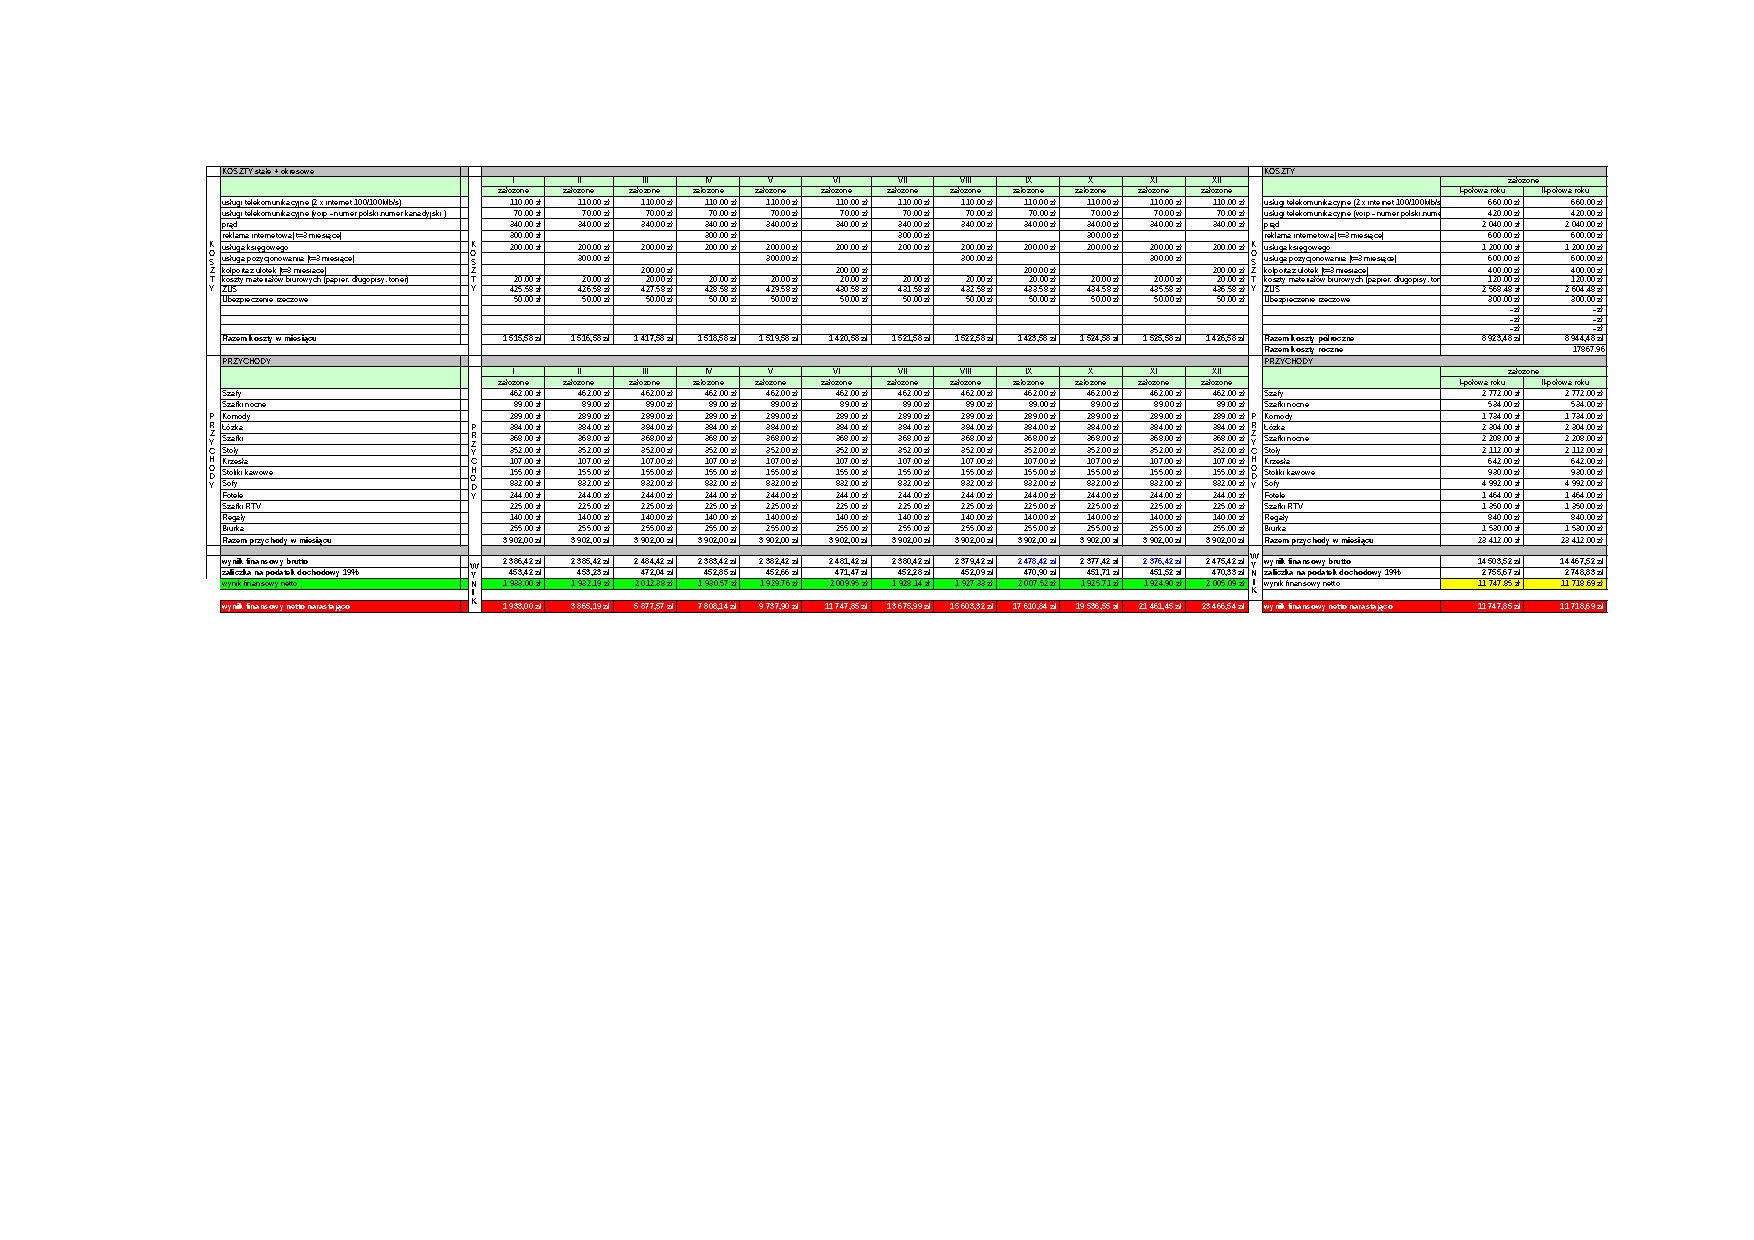
\includepdf[pages={1-},angle=270]{koszty.pdf}

		\section{Planowane przychody}
			
	\par Na potrzeby polityki cenowej przeprowadzona została wstępna analiza rynku, o której mowa była w planie marketingowym. Na jej podstawie można ustalić następujące przychody: 
	
	
	\begin{figure}[H]
        \centering
        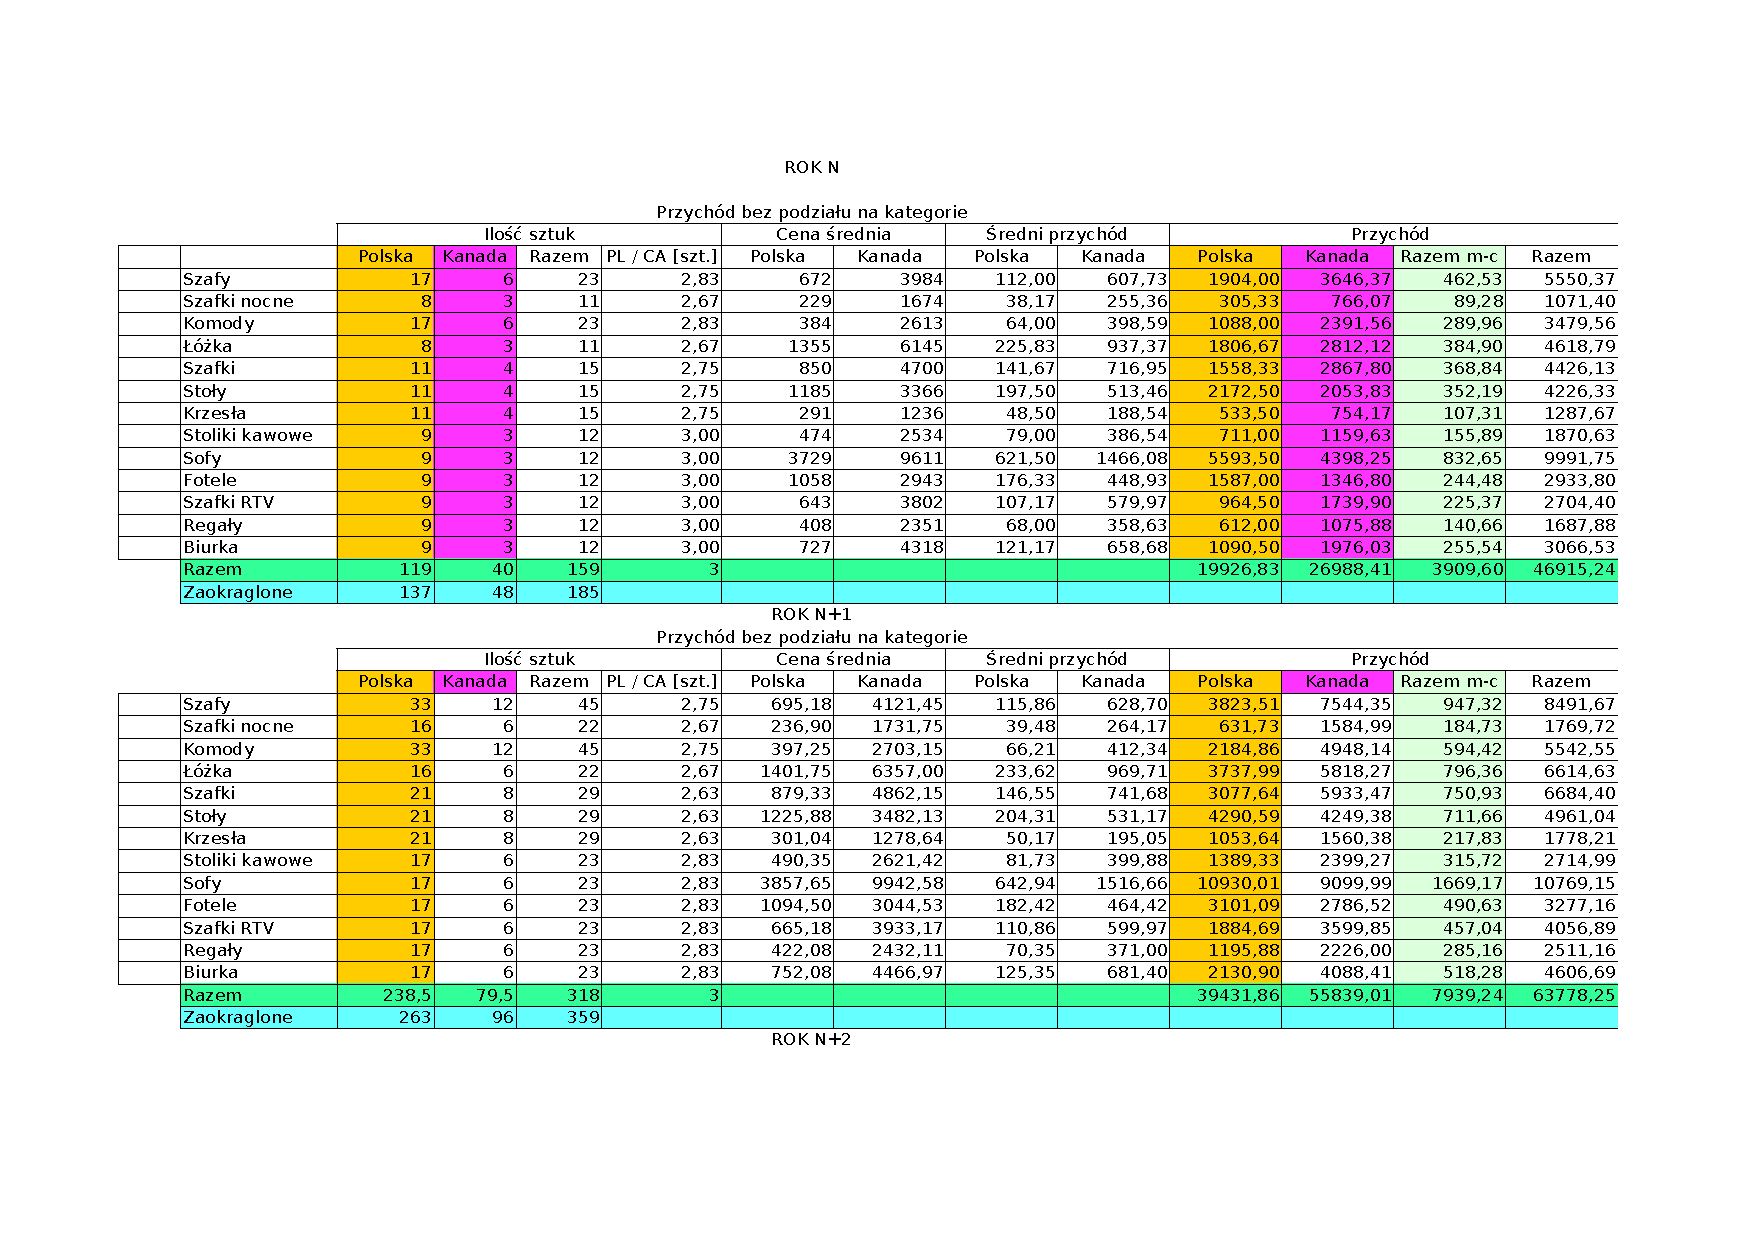
\includegraphics[width=\textwidth,page=1,clip,trim=0 10.75cm 0 0]{prognoza}
        \caption{Tabela przedstawiająca prognozowany zysk}
	\end{figure}
	
	\begin{figure}[H]
        \centering        
        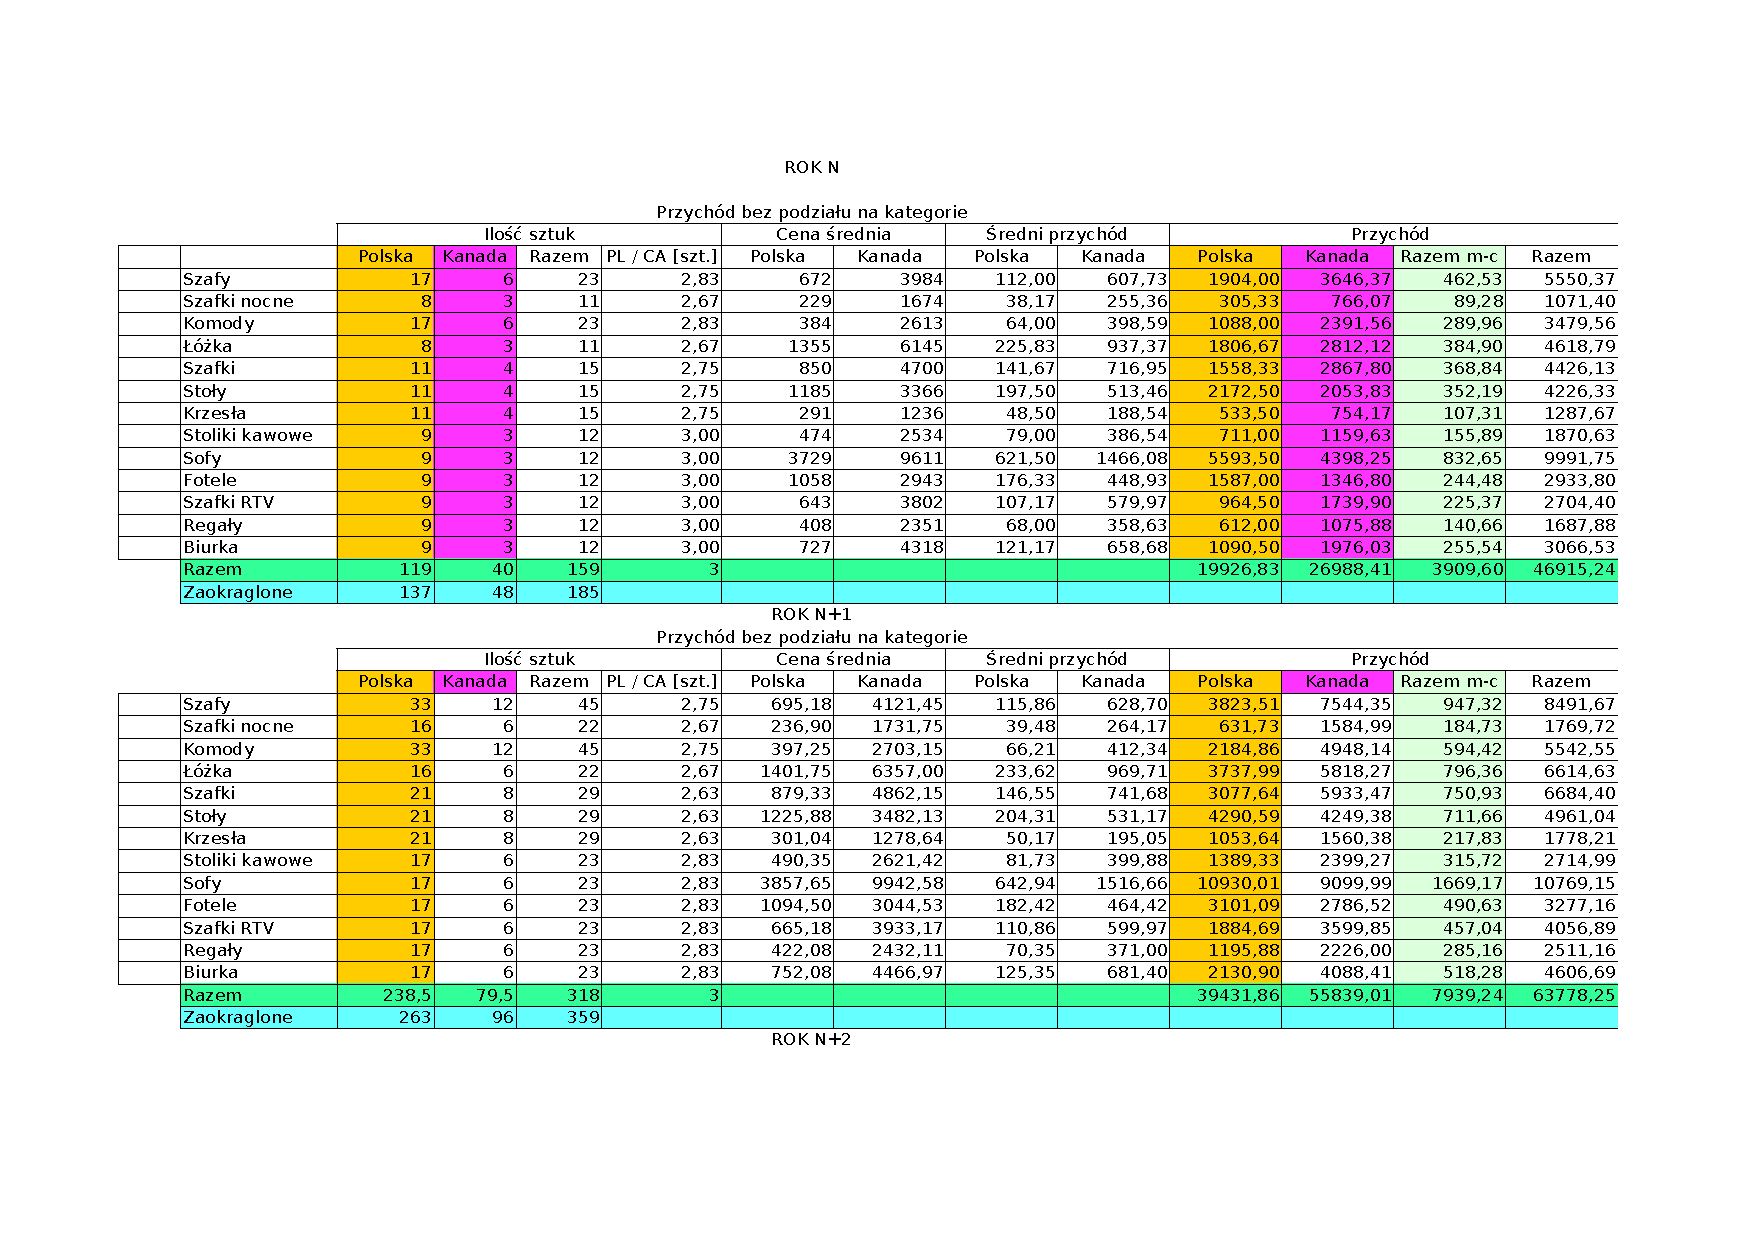
\includegraphics[width=\textwidth,page=1,clip,trim=0 3.55cm 0 10.25cm]{prognoza}
        \caption{Tabela przedstawiająca prognozowany zysk}
	\end{figure}
	
	\begin{figure}[H]
        \centering        
        \includegraphics[width=\textwidth,page=2,clip,trim=0 10.75cm 0 2cm]{prognoza}
        \caption{Tabela przedstawiająca prognozowany zysk}
	\end{figure}
	

		\section{Bilans}
			
	\par Bilans przedstawia zasoby przedsiębiorstwa oraz źródła ich finansowania. Podstawowymi elementami bilansu są aktywa (zasoby przedsiębiorstwa) oraz pasywa (źródła ich finansowania).
	
	\subsubsection{Aktywa}
		\par Aktywa dzielą się na aktywa trwałe i aktywa obrotowe, przy czym kryterium podziału jest okres czasu, przez jaki firma zamierza dane aktywo utrzymywać:

			\begin{itemize}
				\item Aktywa trwałe – aktywa, które nie zużywają się w trakcie jednego cyklu produkcyjnego i które firma zamierza utrzymywać dłużej niż rok.
				\item Aktywa obrotowe – są to aktywa wykorzystywane w jednym cyklu produkcyjnym lub takie, które firma planuje spieniężyć w okresie krótszym niż rok.
			\end{itemize}
			
			\subsubsection{Pasywa}
				\par Pasywa z kolei dzielą się na:

			\begin{itemize}
				\item Kapitały własne – kapitały reprezentujące własne źródła finansowania, takie jak kapitał założycielski bądź zysk zatrzymany.
				\item Kapitały obce (zobowiązania), czyli środki, które firma pożyczyła w celu sfinansowania swojej działalności. Firmy mogą korzystać z bardzo wielu różnych źródeł finansowania. Podstawowym ich podziałem jest podział na zobowiązania długoterminowe i krótkoterminowe. Podobnie jak w przypadku aktywów, kryterium podziału będzie termin zapadalności, a graniczną długością czasu – rok.
			\end{itemize}
 
	\par Tabela poniżej przedstawia bilans mojego sklepu internetowego na lata 2017-2019:
	
	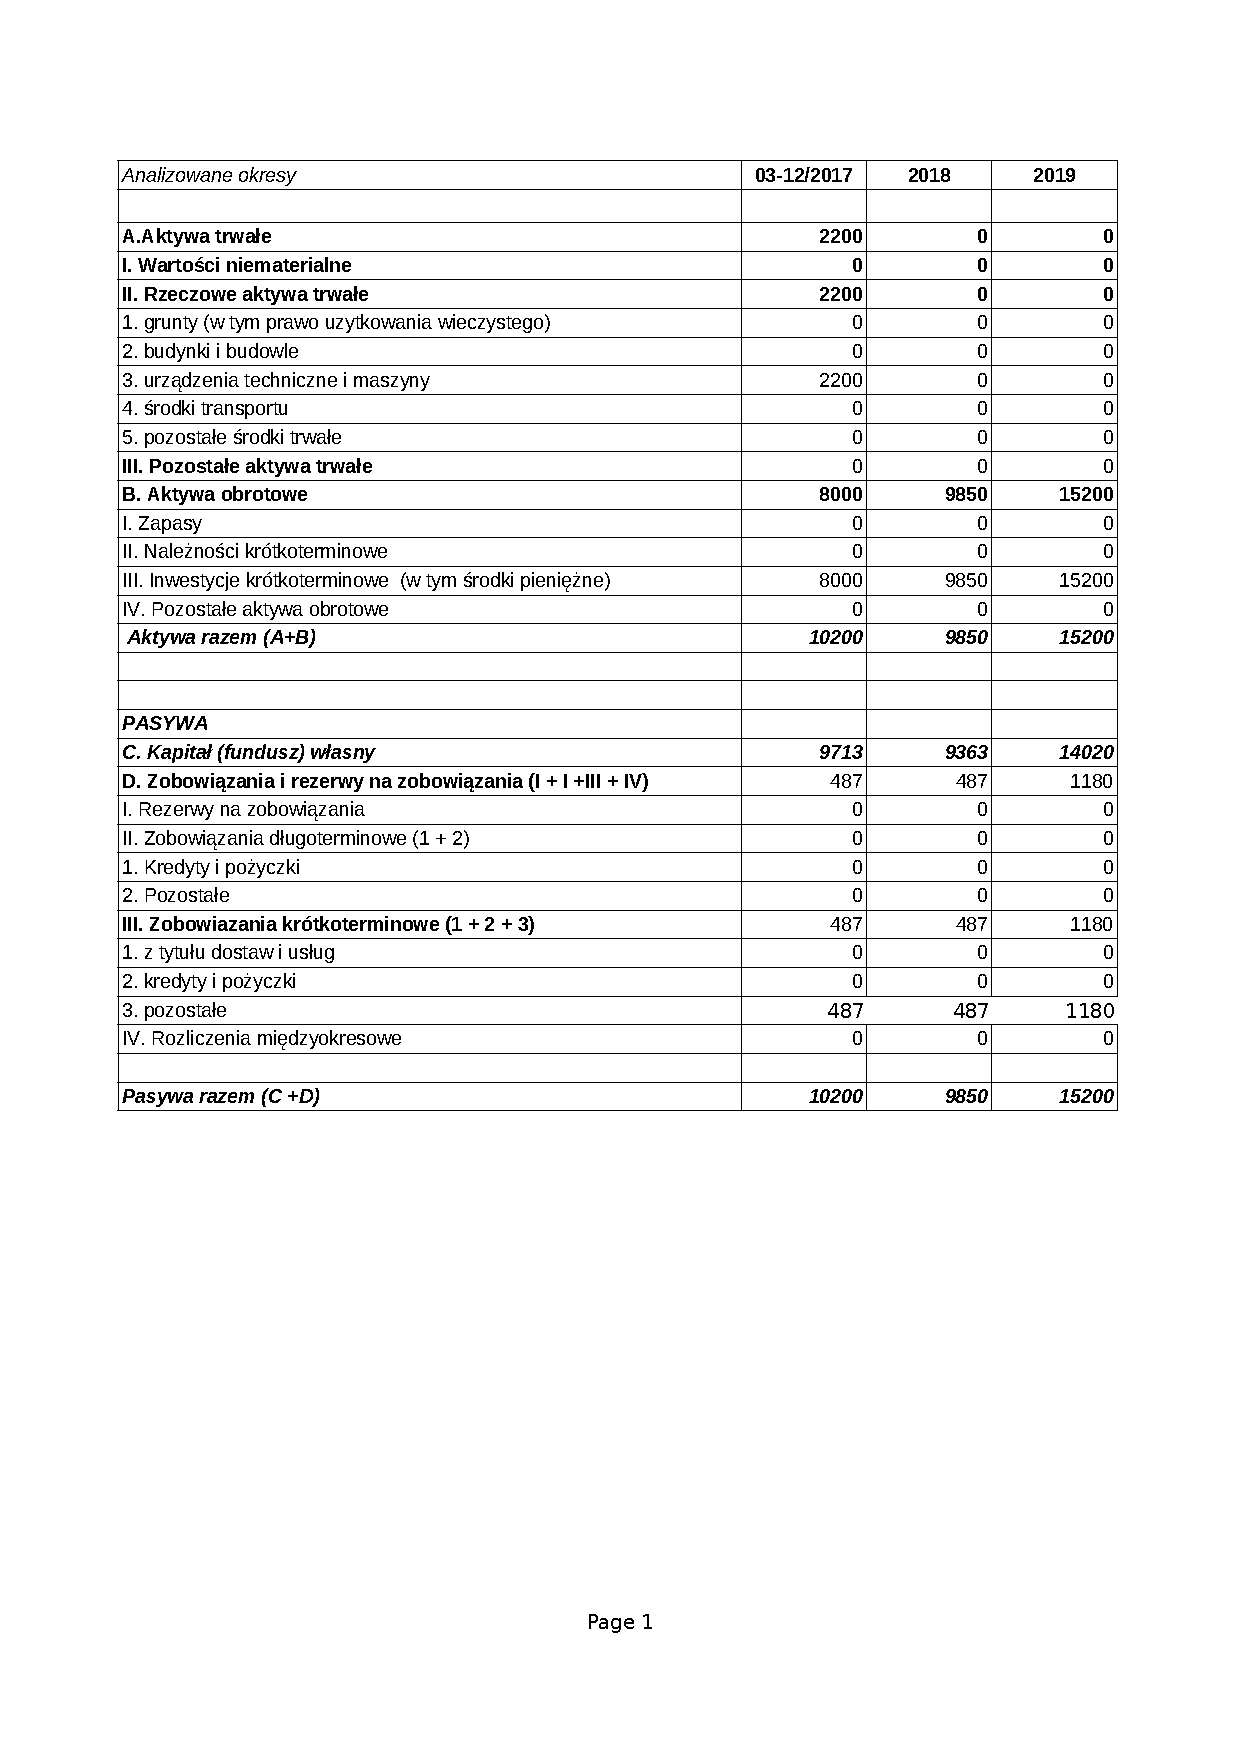
\includepdf[pages={1-},scale=0.9]{bilans.pdf}
	
	\subsubsection{Opis}
		\begin{itemize}
			\item Aktywa trwałe/Rzeczowe aktywa trwałe/urządzenia techniczne i maszyny- kwota 2200 zł dotyczy posiadanego przeze mnie laptopa niezbędnego do prowadzenia sklepu internetowego.
			\item Aktywa obrotowe/Inwestycje krótkoterminowe- kwota 8000 zł odnosi się do posiadanych przeze mnie oszczędności, które przeznaczę na zakup mebli biurowych, reklamę i inne niezbędne rzeczy potrzebne na początku funkcjonowania firmy.
			\item Pasywa/Kapitał własny- kwota 9713 zł to kapital wlasny na pokrycie swoich aktywów.
			\item Pasywa/Zobowiązania krótkoterminowe/Pozostałe- kwota 487 zł to suma składek ZUS z dobrowolnym ubezpieczeniem chorobowym.
			
			
		\end{itemize}	
	
	
	
		





\appendix

	\chapter{Regulamin sklepu internetowego}
		\section{Regulamin polski}
			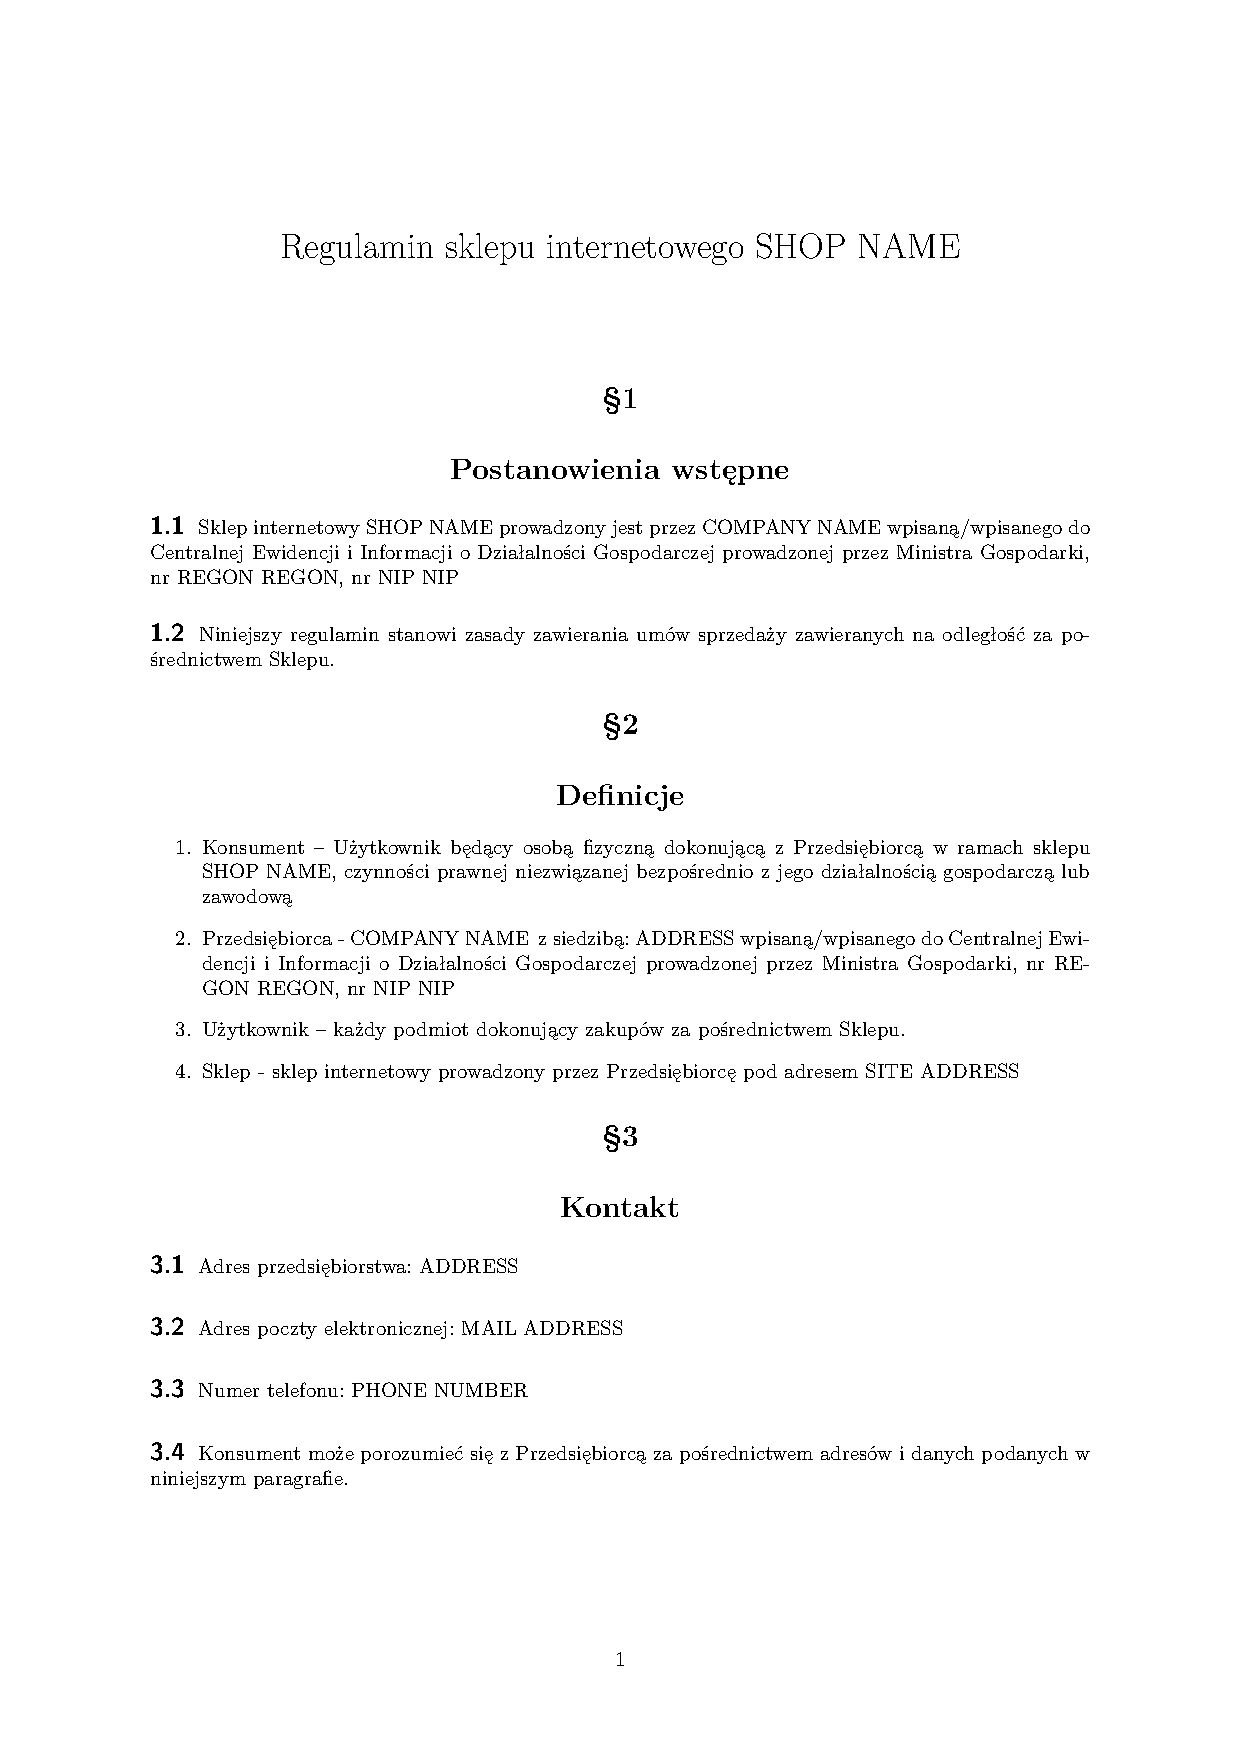
\includepdf[pages={1-},scale=0.85,pagecommand={\thispagestyle{headings}},clip,trim=0mm 25mm 0mm 25mm]{regulamin_PL.pdf}
			
		\section{Regulamin kanadyjski}
			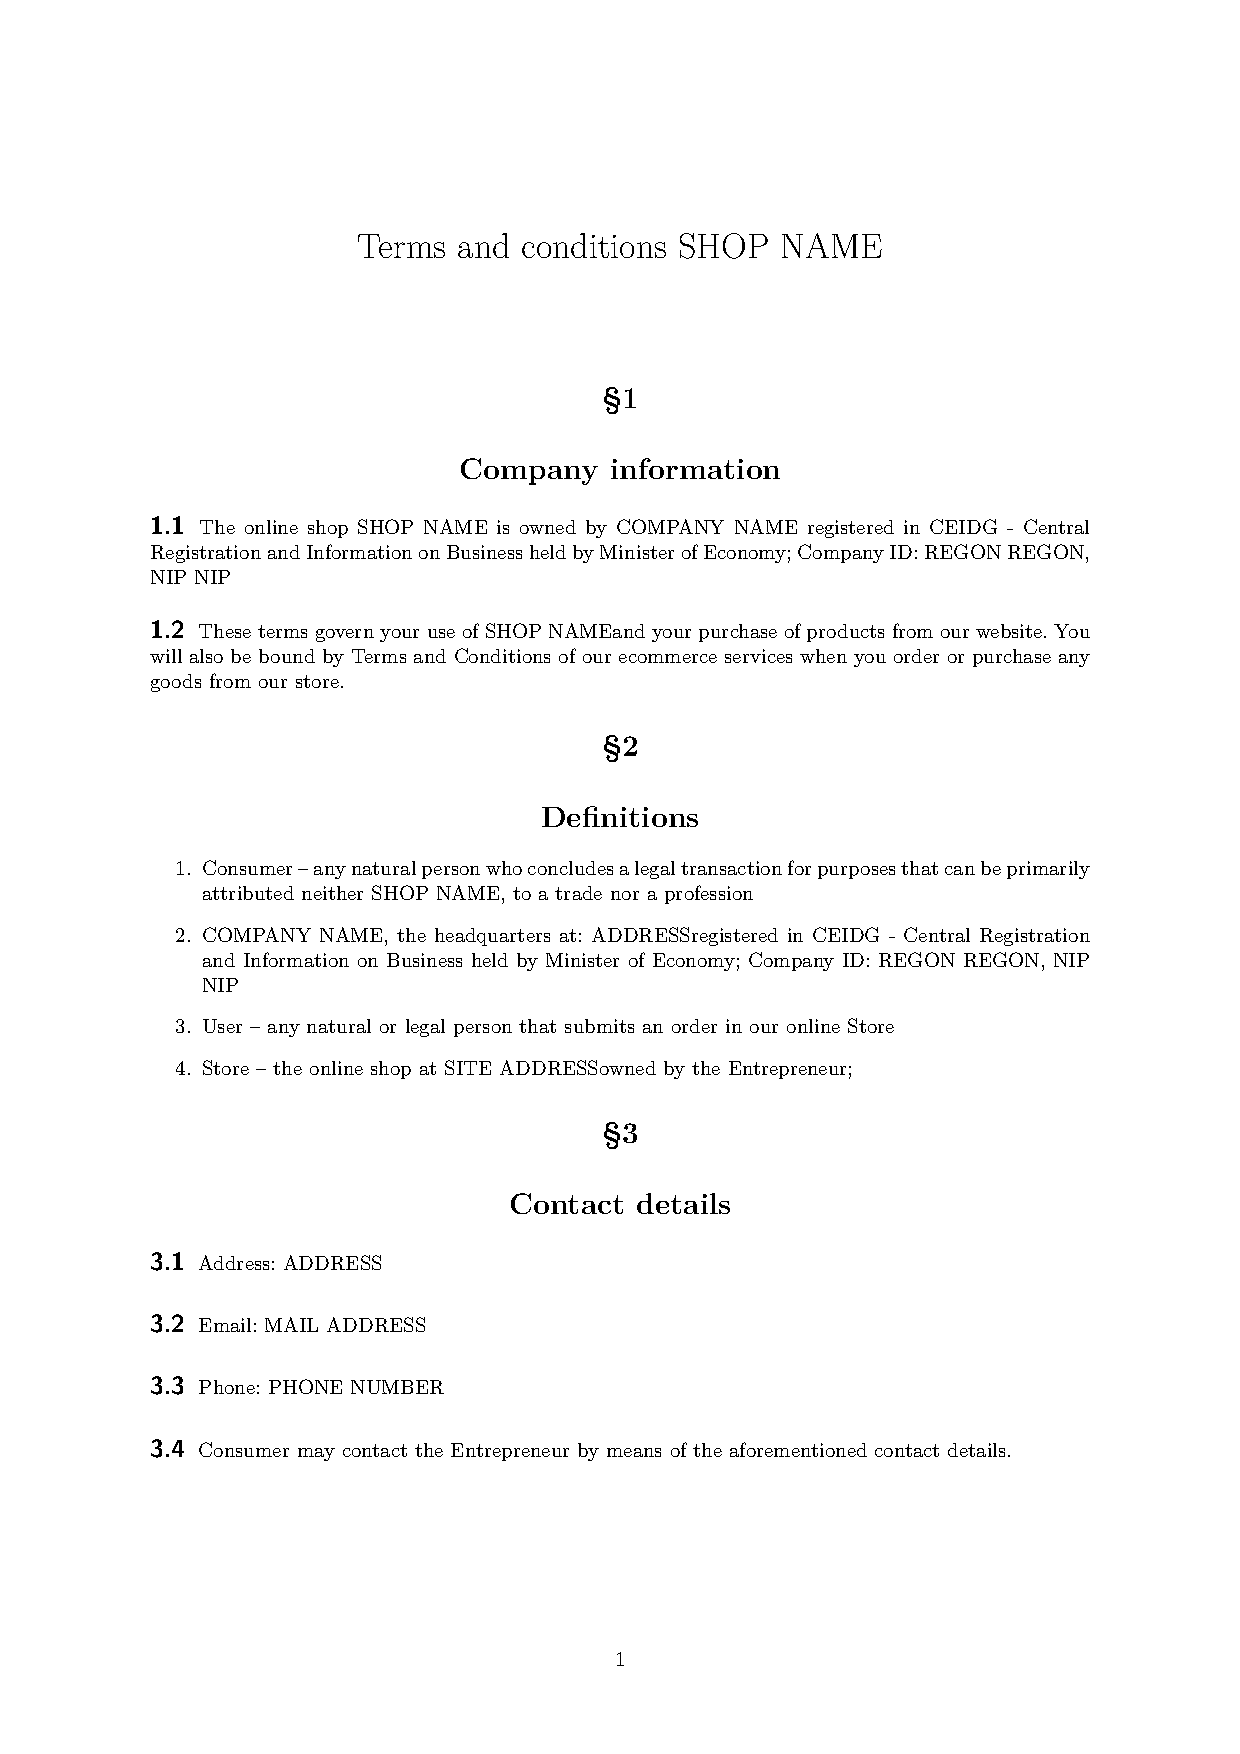
\includepdf[pages={1-},scale=0.85,pagecommand={\thispagestyle{headings}},clip,trim=0mm 25mm 0mm 25mm]{regulamin_EN.pdf}

	\chapter{Polityka cookies}
		\section{Polityka polska}
			
\includepdf[pages={1-},scale=0.85,pagecommand={\thispagestyle{headings}},clip,trim=0mm 25mm 0mm 25mm]{polityka_cookies_PL.pdf}

			\section{Polityka kanadyjska}
				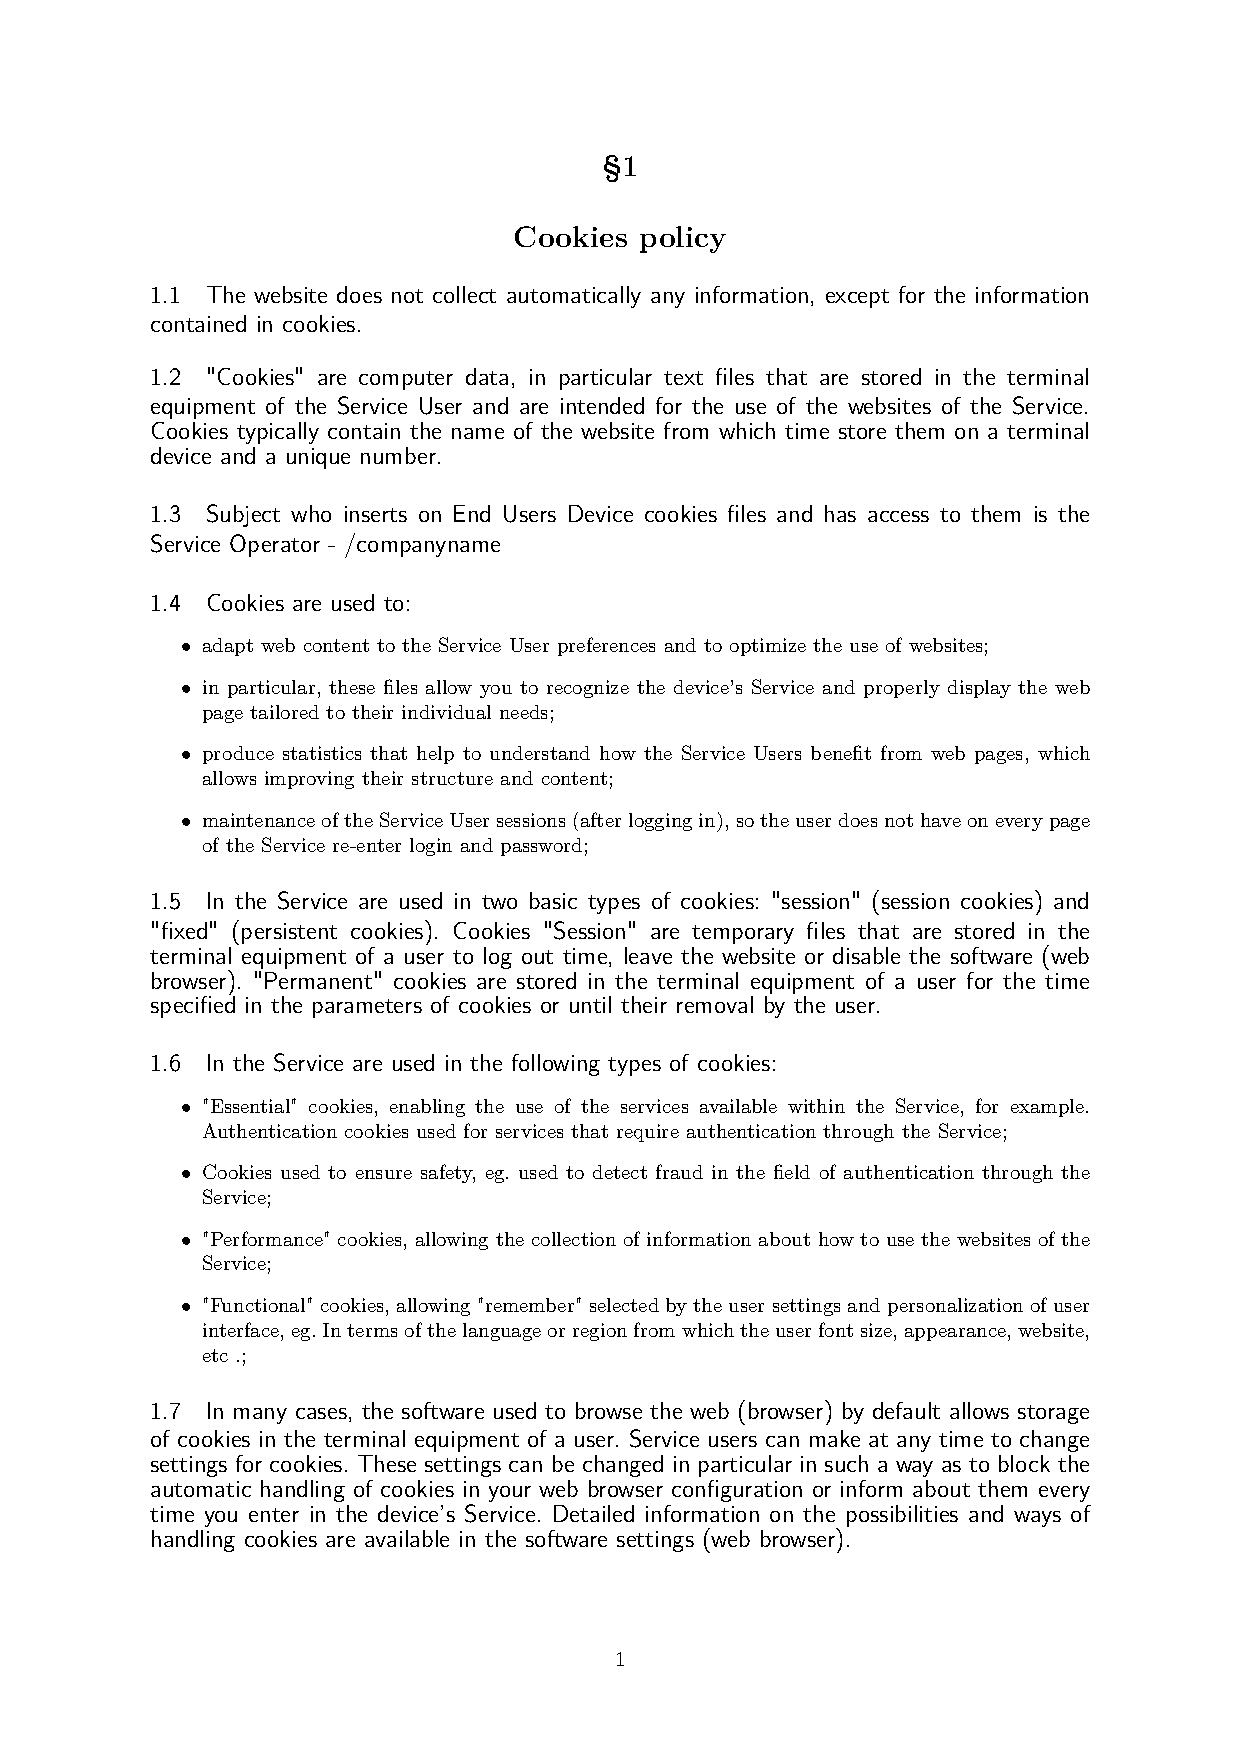
\includepdf[pages={1-},scale=0.85,pagecommand={\thispagestyle{headings}},clip,trim=0mm 25mm 0mm 25mm]{polityka_cookies_EN.pdf}

	\chapter{Karta gwarancyjna}
		\section{Polska karta gwarancyjna}
			
\includepdf[pages={1-},scale=0.85,pagecommand={\thispagestyle{headings}},clip,trim=0mm 25mm 0mm 25mm]{karta_gwarancyjna_PL.pdf}
	
		\section{Kanadyjska karta gwarancyjna}
			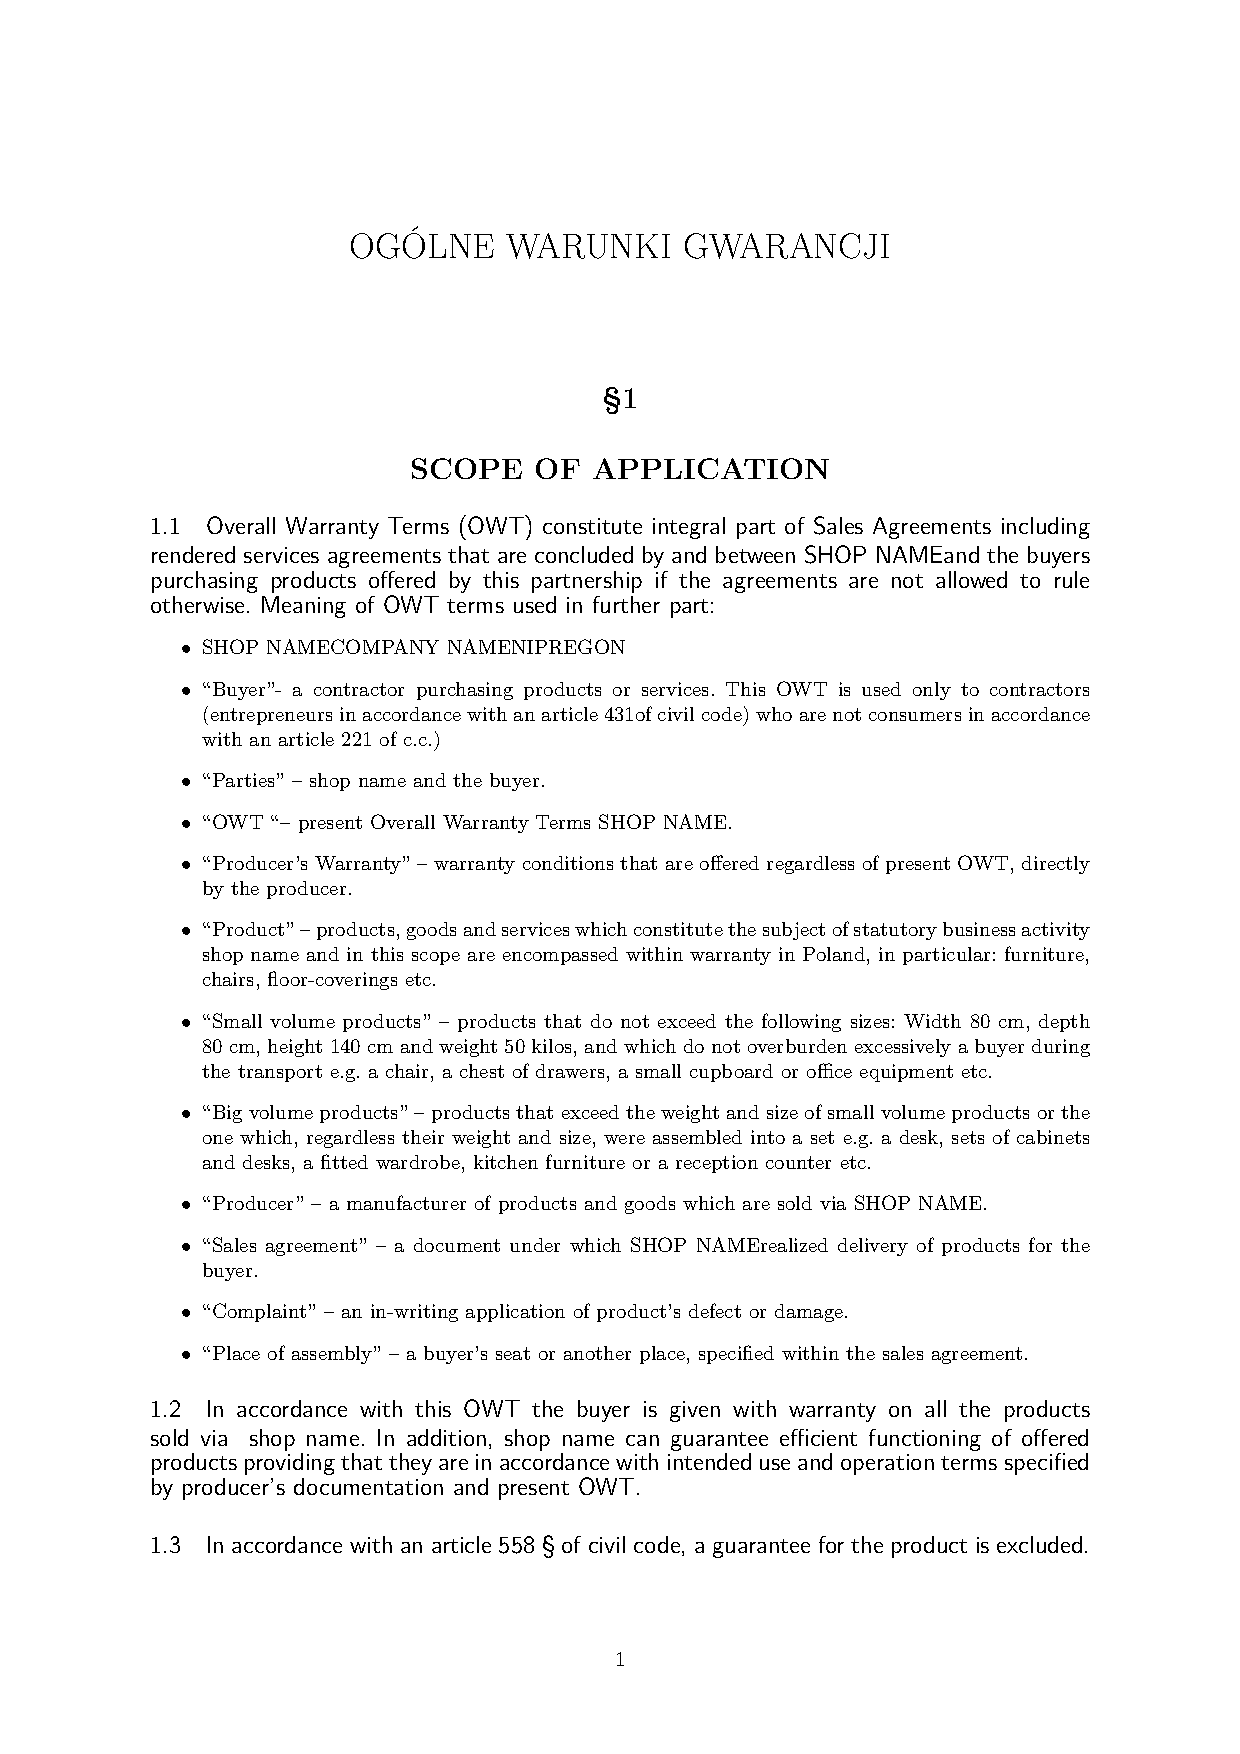
\includepdf[pages={1-},scale=0.85,pagecommand={\thispagestyle{headings}},clip,trim=0mm 25mm 0mm 25mm]{karta_gwarancyjna_EN.pdf}
\end{document}
